% !TeX root = ../../Book1.tex
% 纲要标题：## 附录 C　群论专题简介
% 纲要位置：计划纲要.md，第 885 行。
% BEGIN APPENDIX OUTLINE SYNC
% * 自由积与带合并自由积；右陪集分解、标准串作用与因子嵌入；HNN 构造、标准形与 Britton 引理
% * 自由积的陪集树、有限群不动点及有限子群的共轭包含；字距离与群增长的生成集比较，自由群与有限生成交换群的增长计算
% * 群展示的有限证书与半判定；可判定性的生成集不变性、有效标准形及固定群的不可判定性；稳定子链、Schreier–Sims、Todd–Coxeter 与软件结果的独立核验
% * 有限单群分类与扩张问题的区别；局部结构工具及射影特殊线性群实例，技术子分类见专题文献
% * 转移同态的构造与代表元无关性；Burnside 正规 \(p\)-补定理及正规补群算例
% * 正规 Hall 子群与补群；可解情形的 Schur–Zassenhaus 与 Hall 子群存在、共轭及包含定理，一般 Schur–Zassenhaus 的证明范围明示
% END APPENDIX OUTLINE SYNC

\chapter{群论专题简介}
\label{b1:app:C}
\BookChapterNumber{b1:app:C}

\begin{chapterabstract}
	给群添加关系可能改变其标准形、子群结构和计算难度。本附录从带合并自由积与 HNN 扩张的标准形出发，研究树作用与群增长，并用稳定子链和陪集表处理可核验的群计算。有限群部分先辨析单群分类与扩张问题，再以转移构造正规补群，证明正规 Hall 子群的补群存在性及可解条件下的共轭性，最后建立可解群的 Hall 子群定理。
\end{chapterabstract}

\begin{learninggoals}
	\begin{itemize}
		\item 用泛性质构造带合并自由积与 HNN 扩张，用标准形和 Britton 引理辨认元素。
		\item 根据陪集树计算稳定子群，说明有限子群的限制，并比较自由群与有限生成交换群的增长。
		\item 分清标准形的存在性与有效计算；利用稳定子链筛选置换，核验有限陪集表，并说明算法的停机边界。
		\item 说明有限单群分类回答了什么问题，以及合成因子为何不足以确定原群。
		\item 构造转移同态，使用正规化子条件判断正规 \(p\)-补群的存在，并计算具体转移核。
		\item 通过互素交换核的平均化与有限群归纳证明补群定理，确定 Hall 子群的存在、共轭和包含结论所需的条件。
	\end{itemize}

\end{learninggoals}

设 \(a^2=1\)、\(b^3=1\)，除此之外不规定 \(a,b\) 之间的关系，所得群就是 \(C_2*C_3\)。由自由积标准形，\((ab)^n\) 对每个正整数 \(n\) 都是非空约化字，不等于单位；所以 \(ab\) 有无限阶，群也无限。若再规定 \(ab=ba\)，每个字都能写成 \(a^\varepsilon b^\delta\)，其中 \(0\leq\varepsilon<2\)、\(0\leq\delta<3\)，因而至多有六个元素。另一方面，将 \(a,b\) 分别送到 \(C_2\times C_3\) 的两个标准生成元，给出到这个六阶群的满同态，因此这六个标准形确实不同，所得群同构于 \(C_2\times C_3\)。其中 \(ab\) 的阶为 \(\operatorname{lcm}(2,3)=6\)，所以它又同构于 \(C_6\)。一条交换关系不但把无限群变成有限群，还把原来无限阶的 \(ab\) 变成六阶元素。带合并自由积继续考察“识别已有子群”会改变什么；树上的作用使字的化简获得几何解释，而字问题则把“两个字是否相等”推进到算法能否总给出答案。

\ProseParagraphBreak
前三节问的是如何由因子和关系构造群、辨认元素以及计算相等性。对于有限群，另一种问题是它能够沿正规列分成哪些简单因子。六阶循环群与三个字母上的置换群 \(S_3\) 有同样两个合成因子，却由不同的方式把因子接起来；即使列出全部有限单群，也不能省去扩张方式的研究。单群的分类告诉我们可能出现哪些因子，具体群的构造还须说明这些因子怎样结合。

\ProseParagraphBreak

本附录的前三节以\chapref{b1:ch:08}的自由群、群展示和自由积为基础，从标准形、树作用走到增长和算法。群作用调用\chapref{b1:ch:04}；图论所需的路径和树在使用处说明。合并积与 HNN 标准形、Britton 引理、有限群树作用的不动点、增长计数以及两种群算法的正确性均在本附录证明。字问题不可判定性的计算编码采用证明概要；标准形的存在与有效求解程序的构造是两项不同的任务。

\ProseParagraphBreak
后三节可沿有限群的路线阅读：分类概览使用\chapref{b1:ch:07}的合成列，转移与补群则使用群作用、Sylow 定理、\chapref{b1:ch:06}的半直积与因子集，以及可解群的封闭性质。正规补群使扩张问题具体化：在 \(S_3\) 中，三阶正规子群和二阶补群产生非平凡半直积；在互素交换核上，有限求和又能修正截面，使乘法误差消失。这条路线给出转移、Burnside 正规 \(p\)-补定理及有限可解群 Hall 子群定理的完整证明。一般正规 Hall 子群的补群存在性不要求可解性；共轭性先在核或商群可解的条件下证明，去掉该条件时另行说明所用的奇数阶群定理。

\ProseParagraphBreak
Lyndon 与 Schupp 的《Combinatorial Group Theory》\cite[Chapter I, Sections 1--3, 11; Chapter IV, Sections 1--2]{LyndonSchupp2001}讨论自由群、带合并自由积与 HNN 扩张；其中关于展示和判定问题的章节可另见\cite[Chapter II, Sections 1--2; Chapter IV, Sections 4--5]{LyndonSchupp2001}。有限群及 Mathieu 群的实例可查 Rotman 的《An Introduction to the Theory of Groups》\cite[Chapter 9]{Rotman1995TheoryGroups}。Aschbacher 的《Sporadic Groups》\cite[Preface, pp. ix--xi]{Aschbacher1994SporadicGroups}的序言概述分类名单，Solomon 的综述\cite[Solvable Signalizer Functor Theorem; Gorenstein--Lyons Trichotomy Theorem]{Solomon2001SimpleGroupsHistory}说明相关局部分析在分类中的作用。

% !TeX root = ../../Book1.tex
% 纲要标题：### C.1 自由积与带合并自由积
% 纲要位置：计划纲要.md，第 889 行。
% BEGIN APPENDIX OUTLINE SYNC
% #### C.1.1 自由积的约化字
% #### C.1.2 识别公共子群的构造
% #### C.1.3 标准形与因子的嵌入
% END APPENDIX OUTLINE SYNC

\section{自由积与带合并自由积}
\label{b1:sec:C01}

把两个群放进同一个群中，可以要求它们的元素逐一交换，也可以只保留各自已有的关系。直积与自由积分别对应这两种要求。若两个群还包含一个需要认作相同的子群，就应在自由积中加入识别关系；关键是确认这些关系不会把同一因子中原本不同的元素意外识别。

\subsection{自由积的约化字}
\label{b1:subsec:C01:01}

\cref{b1:lem:free-product-normal-form}已经证明：自由积 \(A*B\) 的每个元素有唯一交替字 \(x_1\cdots x_n\)，各字母来自 \(A\setminus\{1\}\) 或 \(B\setminus\{1\}\)，相邻字母来自不同因子；空字表示单位。这里一个字母可以是因子中的任意非单位元素，不限于某组生成元。化简时把相邻的同因子字母相乘，并删除所得的单位元，直到非单位字母交替为止。两因子的同态可以由\cref{b1:thm:free-product-universal}唯一拼成自由积上的同态，不要求它们的像交换。

\ProseParagraphBreak
例如 \(C_2*C_3=\langle a,b\mid a^2=b^3=1\rangle\)。在字 \((ab)^m\) 中，\(a,b\) 均非单位元，连续字母始终来自不同因子，没有可以相乘化简的相邻字母。因此对每个 \(m>0\)，这个字都约化且非空，由标准形知 \((ab)^m\ne1\)，所以 \(ab\) 有无限阶。两个有限群的自由积可以无限；这与直积 \(C_2\times C_3\cong C_6\) 的情形不同。这个判断来自标准形，不能只从展示中“看不见 \((ab)^m=1\)”便推断其不成立。

\subsection{识别公共子群的构造}
\label{b1:subsec:C01:02}

所谓“公共子群”，可以是同一个抽象群在两个因子中的不同实现，无须原先就是两因子的同一个集合子群。例如取两个无限循环群 \(\langle a\rangle\)、\(\langle b\rangle\)，希望将第一个群中的 \(a^2\) 与第二个群中的 \(b^3\) 认作同一元素，同时保留两个因子中的其他运算。这时取抽象无限循环群 \(C=\langle c\rangle\)，指定嵌入 \(i(c)=a^2\)、\(j(c)=b^3\)，再加入关系 \(a^2=b^3\)。一般构造用两条指定的单同态记录这种要求，识别的是同一个 \(c\in C\) 在两因子中的像 \(i(c),j(c)\)。

\begin{definition}\label{b1:def:amalgamated-free-product}
	设 \(C,A,B\) 为群，\(i:C\hookrightarrow A\)、\(j:C\hookrightarrow B\) 为单同态。把 \(A,B\) 视为自由积中的两个因子，并令
	\[
		N=\bigl\langle\!\bigl\langle i(c)j(c)^{-1}\mid c\in C\bigr\rangle\!\bigr\rangle \trianglelefteq A*B.
	\]
	商群 \((A*B)/N\) 称为沿 \(C\) 的\term[dai-hebing-ziyouji]{带合并自由积}[free product with amalgamation]，记为 \(A*_C B\)。记从两因子到该商群的自然同态为 \(u:A\rightarrow A*_C B\)、\(v:B\rightarrow A*_C B\)。
\end{definition}

\symidx{\(A*_C B\)：沿给定嵌入合并 \(C\) 的自由积}

这里的双尖括号表示正规闭包，即包含所列元素的最小正规子群。若商映射记为 \(\pi\)，则 \(u(a)=\pi(a)\)、\(v(b)=\pi(b)\)；关系 \(i(c)j(c)^{-1}\in N\) 恰使 \(u\bigl(i(c)\bigr)=v\bigl(j(c)\bigr)\)。一旦令这个关系元素在商群中等于 \(1\)，它的每个共轭 \(w\,i(c)j(c)^{-1}w^{-1}\)（\(w\in A*B\)）以及这些共轭及其逆的有限乘积也必须等于 \(1\)。这正是\cref{b1:def:normal-closure}及其后的有限乘积描述中，关系通过共轭与乘积传播的规则。取正规闭包既保证商群所用的核正规，也只加入这些识别所强制的关系。

\ProseParagraphBreak
下标 \(C\) 还隐含了两条嵌入 \(i,j\)；只知道三个抽象群，并不足以指定这个构造。定义立即给出 \(ui=vj\)，但加入关系的商构造本身并不排除因子中的非单位元素被送到单位元，所以 \(u,v\) 的单射性还需要下一小节的证明。对于任一群 \(H\) 及同态 \(f:A\to H\)、\(g:B\to H\)，条件 \(fi=gj\) 表示：对每个 \(c\in C\)，两条路径给出同一个像 \(f(i(c))=g(j(c))\)。泛性质断言，这样的两条同态能由商群上的唯一同态同时得到。

\begin{proposition}\label{b1:prop:amalgam-universal}
	设 \(C,A,B,H\) 为群，\(i:C\hookrightarrow A\)、\(j:C\hookrightarrow B\) 为单同态，\(A*_C B\) 是沿 \(i,j\) 构造的带合并自由积，\(u:A\rightarrow A*_C B\)、\(v:B\rightarrow A*_C B\) 为自然同态。若同态 \(f:A\rightarrow H\)、\(g:B\rightarrow H\) 满足 \(fi=gj\)，则存在唯一同态 \(h:A*_C B\rightarrow H\) 满足 \(hu=f\)、\(hv=g\)。
\end{proposition}

\begin{proof}
	自由积的泛性质给出唯一同态 \(\widetilde h:A*B\rightarrow H\)，在两因子上的限制分别是 \(f,g\)。对每个 \(c\in C\)，有
	\[
		\widetilde h\bigl(i(c)j(c)^{-1}\bigr) =f\bigl(i(c)\bigr)g\bigl(j(c)\bigr)^{-1}=1.
	\]
	核是正规子群，故包含定义中的 \(N\)。由\cref{b1:thm:quotient-universal}，\(\widetilde h\) 唯一地通过商群下降为 \(h\)。两因子的像生成商群，因此任何满足所述限制的同态都只能是这个 \(h\)。
\end{proof}

当 \(C=1\) 时，没有额外识别，得到普通自由积。若 \(C=A=B\) 且两嵌入均为恒等，两个因子的对应元素全被识别，所以自然同态 \(u,v:A\to A*_A A\) 相等。两者的像生成商群，故 \(u\) 满射；泛性质又给出 \(h:A*_A A\to A\)，满足 \(hu=hv=\operatorname{id}_A\)，所以 \(u\) 也单射。于是 \(u\) 与 \(h\) 互逆，给出 \(A*_A A\cong A\)。

\subsection{标准形与因子的嵌入}
\label{b1:subsec:C01:03}

利用 \(i,j\) 可把 \(C\) 分别视为 \(A,B\) 的子群。为每个右陪集 \(Ca\)、\(Cb\) 选一个代表，得到代表集 \(T_A,T_B\)，均以 \(1\) 代表 \(C\) 本身。若 \(t\) 代表 \(Ca\)，则 \(Ca=Ct\)，从而 \(a=ct\)；使用这种右陪集约定，\(C\) 系数位于代表的左边。因此每个因子元素都有唯一分解 \(ct\)，其中 \(c\in C\)，\(t\) 属于该因子的代表集。这里对非空陪集族应用\cref{b1:def:A-choice}中的选择公理，再把单位陪集的代表改取为 \(1\)。这保证代表集存在，却没有给出从输入元素求出 \(c,t\) 的算法；有效计算还需另有可执行的陪集分解方法。

\ProseParagraphBreak
这一步的唯一性来自两个不同层次。给定 \(a\in A\)，陪集 \(Ca\) 先确定唯一代表 \(t\in T_A\)，再由 \(a=ct\) 确定 \(c=at^{-1}\in C\)。不同因子的代表仍保留各自的标记；它们只是各因子元素的一种写法。我们要进一步证明，在合并所得的群中，也可以用这些代表写出唯一的交替表达式。由于 \(C\) 未必在因子的中心，不能简单地把一个乘积中的所有 \(C\) 元素交换到最左边；下述证明会在每次左乘时重新作陪集分解。

\begin{theorem}[带合并自由积的标准形]\label{b1:thm:amalgam-normal-form}
	设 \(C,A,B\) 为群，\(i:C\hookrightarrow A\)、\(j:C\hookrightarrow B\) 为单同态，并通过 \(i,j\) 把 \(C\) 分别视为 \(A,B\) 的子群。分别选取 \(C\) 在 \(A,B\) 中的右陪集代表集 \(T_A,T_B\)，并以 \(1\) 代表单位陪集。则每个 \(A*_C B\) 中的元素唯一表示为
	\[
		c t_1\cdots t_n, \qquad c\in C,\quad t_k\in(T_A\setminus\{1\})\sqcup(T_B\setminus\{1\}),
	\]
	其中各 \(t_k\) 交替来自两代表集，允许 \(n=0\)。特别地，自然映射 \(A\rightarrow A*_C B\)、\(B\rightarrow A*_C B\) 均单射，其像的交恰为 \(C\) 的像。
\end{theorem}

\begin{proof}
	只证明每个字都能化成这种形式，还不足以排除两个不同的标准串在商群中相等。为证明唯一性，我们构造一个群作用，使每个候选标准串都把同一个基点送到该串所标记的位置。不同串给出不同位置，而同一群元素在基点上的作用只能有一个值，因而可以用这个作用区分标准串。

	令 \(\Omega\) 为所有满足定理条件的有限有序串 \((c;t_1,\ldots,t_n)\) 组成的集合。此时相等只表示长度相同、各位置的符号相同，尚未使用商群中的相等关系。没有代表项且 \(c=1\) 的串记为 \(\omega_0=(1;)\)。对 \(a\in A\)，定义映射 \(L_a:\Omega\rightarrow\Omega\)。若首个代表 \(t_1\) 来自 \(T_A\)，则 \(a,c,t_1\) 全在 \(A\) 中，左乘 \(a\) 后可以直接合并这个前缀，代表 \(t_1\) 也可能被消去。在 \(A\) 中把 \(act_1\) 唯一分解为 \(c't'\)，并令
	\[
		L_a(c;t_1,t_2,\ldots,t_n)=(c';t',t_2,\ldots,t_n).
	\]
	若原串没有代表项，或 \(t_1\) 来自 \(T_B\)，则先把 \(ac\) 分解为 \(c't'\)，再把新得到的 \(A\) 代表插在原代表串之前，令
	\[
		L_a(c;t_1,\ldots,t_n)=(c';t',t_1,\ldots,t_n).
	\]
	这两个公式中，若 \(t'=1\)，均删去该代表项。所得串仍交替：第一种情形中余下的首项 \(t_2\) 若存在，便属于另一因子；第二种情形中原来的 \(t_1\) 若存在，也属于另一因子。对 \(b\in B\) 交换两因子的角色，定义 \(L_b\)。

	对同一因子中的 \(a,a'\)，有 \(L_aL_{a'}=L_{aa'}\)，其中左边先作用 \(L_{a'}\)。这个等式取决于因子中 \(ct\)-分解的唯一性。若原串以该因子的代表开头，设第一次分解为 \(a'ct_1=c't'\)。当 \(t'\ne1\) 时，第二次分解 \(ac't'=aa'ct_1\)；当 \(t'=1\) 时，原首代表已消去，第二次分解 \(ac'=aa'ct_1\)，余下的代表串从另一因子开始。两种情形的前缀都是同一个元素 \(aa'ct_1\)，所以与一次作用 \(L_{aa'}\) 得到的分解相同。若原串不以该因子开头，只需将这里的 \(ct_1\) 换成 \(c\)，两次操作最终分解的就是 \(aa'c\)。又 \(L_1\) 是恒等映射，故 \(L_{a^{-1}}\) 是 \(L_a\) 的逆，得到同态 \(A\rightarrow S_\Omega\)，其中 \(S_\Omega\) 是集合 \(\Omega\) 上的全体自双射所成的群；\(B\) 亦然。

	对于 \(c_0\in C\)，若首代表来自正在使用的因子，则 \(c_0ct_1\) 已有分解 \((c_0c)t_1\)；若首代表来自另一因子或不存在，则 \(c_0c\in C\) 的代表为 \(1\)。因此两作用都只把首项 \(c\) 改成 \(c_0c\)，在公共子群上相容。以 \(H=S_\Omega\) 应用\cref{b1:prop:amalgam-universal}，遂得到 \(A*_C B\) 在 \(\Omega\) 上的作用。

	任意因子字从右向左依次作用于 \(\omega_0\)，每一步的前缀分解都在商群中保持元素不变，所以输出串表示原元素。这证明存在性。另一方面，标准串对应的群元素 \(ct_1\cdots t_n\) 作用于 \(\omega_0\) 时，先加入 \(t_n\)，再加入 \(t_{n-1}\)，依次进行；因代表交替，过程中没有同因子合并。最后左乘 \(c\)，得到
	\[
		(ct_1\cdots t_n)\cdot\omega_0=(c;t_1,\ldots,t_n).
	\]
	如果两个标准串表示同一群元素，它们在已经构造好的群作用中必给出同一个置换，在 \(\omega_0\) 上的取值也相同，故串完全相同。这证明唯一性。

	因子中的元素 \(ct\) 只有在 \(c=t=1\) 时才等于单位，故两自然映射单射。若一个 \(A\) 中的元素等于一个 \(B\) 中的元素，标准串唯一性迫使两者的非单位代表都不出现，因而均属于 \(C\)。
\end{proof}

例如取 \(A=\langle a\rangle\cong\mathbb Z\)、\(B=\langle b\rangle\cong\mathbb Z\)，把 \(C\cong\mathbb Z\) 的生成元分别送到 \(a^2,b^3\)。则
\[
	A*_C B\cong\langle a,b\mid a^2=b^3\rangle.
\]
可取 \(T_A=\{1,a\}\)、\(T_B=\{1,b,b^2\}\)。记公共元素 \(z=a^2=b^3\)，标准形是 \(z^m t_1\cdots t_n\)。这既说明两个无限循环因子没有被压缩，也给出检验元素是否相等的方法；其中 \(z\) 与 \(a,b\) 都交换，故属于整个群的中心。

\ProseParagraphBreak
例如左乘 \(a\) 于标准形 \(z^mab^2\)，首两个 \(a\) 合并为 \(z\)，结果为 \(z^{m+1}b^2\)；左乘 \(b\) 于 \(z^ma\)，则得到 \(z^mba\)。在第一个计算中，代表项 \(a\) 消失；在第二个计算中，多出了一个来自另一因子的代表项。这正是证明中两种前缀操作的具体情形。对任意输入字重复这些步骤即可化简；其有效计算在\subsecref{b1:subsec:C03:02}中继续说明。

\ProseParagraphBreak
上例的公共元素 \(z\) 恰在中心，不能用它代替一般的前缀分解。再取两份 \(S_3\)：
\[
	A=\langle r,s\mid r^3=s^2=1,\ srs=r^{-1}\rangle, \qquad B=\langle t,u\mid t^3=u^2=1,\ utu=t^{-1}\rangle.
\]
沿同构 \(\langle s\rangle\cong\langle u\rangle\) 合并后，把两者在 \(A*_{C_2}B\) 中的公共像仍记为 \(s\)。可取右陪集代表集 \(T_A=\{1,r,r^2\}\)、\(T_B=\{1,t,t^2\}\)。在标准串 \((s;t)\) 上左乘 \(r\) 时，关系 \(srs=r^{-1}\) 给出 \(rs=sr^2\)，所以
\[
	L_r(s;t)=(s;r^2,t).
\]
若把 \(r\) 与 \(s\) 当作可交换元素，便会误得 \((s;r,t)\)；两个串的代表项不同，按标准形定理表示不同元素。一般而言，把公共子群系数移回左端需要重新作 \(ct\)-分解，代表项可能随之改变，不能将这一步理解为把所有 \(C\) 元素与代表逐一交换。

% !TeX root = ../../Book1.tex
% 纲要标题：### C.2 树作用与几何群论
% 纲要位置：计划纲要.md，第 908 行。
% BEGIN APPENDIX OUTLINE SYNC
% #### C.2.1 自由积的陪集树
% #### C.2.2 有限群作用的不动点
% #### C.2.3 字长与群的几何
% * 新增小节状态：初稿已完成；原有内容保留，新增范围尚未正式审核。
% #### C.2.4 群增长与生成集比较
% #### C.2.5 自由群与交换群增长
% END APPENDIX OUTLINE SYNC

\section{树作用与几何群论}
\label{b1:sec:C02}

自由积的交替字可以用沿图行走来解释：相邻字母来自不同因子，对应路径不断向前而不立即沿原边退回。下面构造这样一个图，再用标准形证明它没有回路。

\ProseParagraphBreak
所用图由顶点、边及每条边的两个端点组成，边不指定方向。顶点的度是与它相接的边数；同时置换顶点和边、并保持端点关系的映射称为图自同构。一条路径记录依次经过的顶点与相邻边，其长度是边数；首尾顶点相同时，它是闭路径。若连续两步沿同一条边走过去再走回来，这两步构成回折，将它们删去就是消去回折。若路径的顶点不重复，称其为简单路径；长度为正、首尾相同、其余顶点不重复且不立即往返的闭路径称为回路。

\ProseParagraphBreak
树是连通而无回路的图，因此任意两顶点间恰有一条简单路径：连通性保证存在，若有两条不同的简单路径，先沿它们的共同起始部分走到首次分开的顶点，再沿第一条路径走到它与第二条路径余下部分首次相遇的顶点。两次相遇之间的两段路径没有共同内点，且起始边不同；沿一段前进、另一段倒退便得到没有回折的回路，矛盾。即使一棵树只有两个顶点 \(v,w\) 和连接它们的一条边，也能沿这条边走出闭路径 \(v\to w\to v\)；它只是一次回折，消去后得到长度零的路径，并不是回路。群在图上的作用，就是把每个群元素表示为一个图自同构，并要求这种表示保持群乘法。

\subsection{自由积的陪集树}
\label{b1:subsec:C02:01}

令 \(G=A*B\)。为把交替字解释为路径，我们希望右乘一个 \(A\) 中的字母时，前后的两条边在同一个 \(A\) 型顶点相接；右乘 \(B\) 中的字母时，则在 \(B\) 型顶点相接。右乘 \(A\) 中的元素恰好保持左陪集 \(gA\)，所以构造图 \(T\)：顶点集是不相交并 \(G/A\sqcup G/B\)，每个 \(g\in G\) 给出一条边，连接 \(gA\) 与 \(gB\)。这里 \(G/A\)、\(G/B\) 只是左陪集的集合，不要求因子正规，也没有赋予它们商群结构。即使两个因子抽象同构，也保留两种顶点类型，分别称为 \(A\) 型和 \(B\) 型。

\ProseParagraphBreak
这个定义同时记录了“哪些群元素相差一个因子元素”。编号为 \(g\) 与 \(g'\) 的两条边在一个 \(A\) 型顶点相接，当且仅当
\[
	gA=g'A \quad\Longleftrightarrow\quad A=g^{-1}g'A \quad\Longleftrightarrow\quad g^{-1}g'\in A;
\]
\(B\) 型顶点相应记录 \(B\) 中的差别。群元素 \(h\) 的作用是把顶点 \(gA\)、\(gB\) 送到 \(hgA\)、\(hgB\)，把编号为 \(g\) 的边送到编号为 \(hg\) 的边。这些规则保持端点关系，并由群乘法的结合律给出群作用。

\begin{proposition}\label{b1:prop:free-product-coset-tree}
	设 \(A,B\) 为群，\(G=A*B\)。令图 \(T\) 的顶点集为 \(G/A\sqcup G/B\)，并对每个 \(g\in G\) 设置一条连接 \(gA\) 与 \(gB\) 的边；\(G\) 以左乘作用在顶点和边上。则 \(T\) 是树，顶点 \(gA,gB\) 的稳定子群分别为 \(gAg^{-1},gBg^{-1}\)，每条边的稳定子群均为单位群。
\end{proposition}

\begin{proof}
	边 \(g\) 与边 \(ga\)（\(a\in A\)）有公共端点 \(gA\)，边 \(g\) 与边 \(gb\)（\(b\in B\)）有公共端点 \(gB\)。给定 \(g=x_1\cdots x_n\) 的交替字，依次经过编号为
	\[
		1,\ x_1,\ x_1x_2,\ \ldots,\ x_1\cdots x_n=g
	\]
	的边：每次右乘 \(x_i\)，都经由其所属因子对应的顶点到达下一条边。这给出从单位边到边 \(g\) 的路径；又每个顶点都是某条边的端点，故图连通。

	若有回路，按次序记边为 \(g_0,g_1,\ldots,g_{m-1},g_m=g_0\)，并令 \(x_i=g_{i-1}^{-1}g_i\)。相邻边在 \(A\) 型或 \(B\) 型顶点相交，故 \(x_i\) 属于相应因子；回路不立即沿原边退回，所以相邻边不同，从而 \(x_i\ne1\)。顶点类型沿回路交替，因此 \(x_1\cdots x_m\) 是非空约化字。另一方面，中间因子逐一抵消给出
	\[
		x_1\cdots x_m =(g_0^{-1}g_1)(g_1^{-1}g_2)\cdots(g_{m-1}^{-1}g_m) =g_0^{-1}g_m=1,
	\]
	与\cref{b1:lem:free-product-normal-form}的非空约化字非单位相矛盾。故图无回路。

	等式 \(hgA=gA\) 当且仅当 \(g^{-1}hg\in A\)，给出第一个稳定子群公式；将 \(A\) 换成 \(B\) 得到第二个公式。边按群元素本身编号，\(hg=g\) 迫使 \(h=1\)，故边稳定子群平凡。
\end{proof}

取 \(A=C_2=\langle a\mid a^2=1\rangle\)、\(B=C_3=\langle b\mid b^3=1\rangle\)。在\cref{b1:fig:free-product-coset-tree}中，单位边连接 \(A\) 与 \(B\)；边 \(a\) 连接 \(A\) 与 \(aB\)，边 \(b,b^2\) 分别连接 \(B\) 与 \(bA,b^2A\)。一般地，与 \(gA\) 相接的边恰以 \(ga\) 为编号，其中 \(a\in A\)，所以 \(A\) 型顶点的度为二；\(B\) 型顶点的度为三。无限群 \(C_2*C_3\) 因而作用在局部有限的无限树上，这里的“局部有限”是指每个顶点的度都有限。

\begin{figure}[htbp]
	\centering
	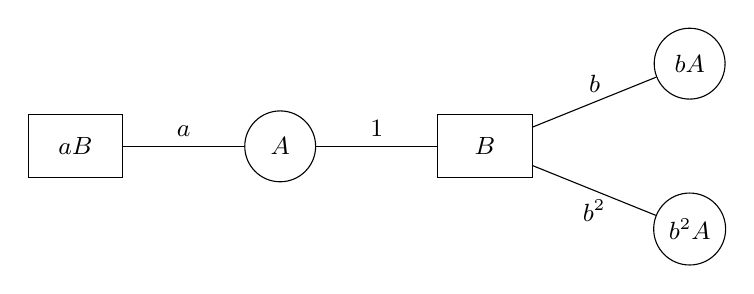
\begin{tikzpicture}[x=1cm,y=1cm,every node/.style={font=\small}]
		\node[draw,rectangle,minimum width=12mm,minimum height=8mm] (aB) at (-4,0) {\(aB\)};
		\node[draw,circle,minimum size=9mm] (A) at (-1.4,0) {\(A\)};
		\node[draw,rectangle,minimum width=12mm,minimum height=8mm] (B) at (1.2,0) {\(B\)};
		\node[draw,circle,minimum size=9mm] (bA) at (3.8,1.05) {\(bA\)};
		\node[draw,circle,minimum size=9mm] (bbA) at (3.8,-1.05) {\(b^2A\)};
		\draw (aB)--node[above] {\(a\)} (A);
		\draw (A)--node[above] {\(1\)} (B);
		\draw (B)--node[above] {\(b\)} (bA);
		\draw (B)--node[below] {\(b^2\)} (bbA);
	\end{tikzpicture}
	\caption[自由积陪集树的局部]{\(C_2*C_3\) 陪集树中单位边附近的部分。圆形表示 \(A\) 型顶点，方形表示 \(B\) 型顶点；顶点标签是左陪集，边标签是群元素。边界处的顶点仍继续向外连接。}
	\label{b1:fig:free-product-coset-tree}
\end{figure}

这棵陪集树与 \(G\) 的 Cayley 图不同。后者的顶点是群元素，左乘作用的顶点稳定子群平凡；前者的顶点是陪集，\(gA,gB\) 的稳定子群分别为 \(gAg^{-1},gBg^{-1}\)。因此，陪集树将因子及其共轭子群表示为顶点稳定子群，下一小节正会利用这一点研究自由积中的有限子群。例如 \(C_2*C_3\) 关于 \(\{a,b\}\) 的 Cayley 图中，关系 \(b^3=1\) 给出由 \(1,b,b^2\) 构成的三角形，陪集图却是树。一般的带合并自由积也有以 \(G/C\) 为边集的类似树。

\subsection{有限群作用的不动点}
\label{b1:subsec:C02:02}

设群 \(G\) 作用在树 \(T\) 上。若不存在保持某条边却交换其两个端点的群元素，则称该作用\term[wu-fanzhuan-shuzuoyong]{无反转}[without inversions]。上面的陪集树作用保持顶点类型，因而无反转。若某个元素交换一条边的两个端点，在这条边中点加入一个顶点后，它会固定中点并交换两条新边，因而不会反转其中任何一条。对每条边都这样细分，并把原图自同构延拓到中点，就得到无反转作用：每条新边都有一个旧顶点和一个新中点，而群作用保持这两类顶点。

\begin{theorem}\label{b1:thm:finite-group-tree-fixed-point}
	设有限群 \(G\) 以无反转方式作用在非空树 \(T\) 上。则 \(T\) 中存在被 \(G\) 的每个元素固定的顶点。
\end{theorem}

\begin{proof}
	取顶点 \(v\)。因为 \(G\) 有限，其轨道 \(Gv\) 有限。若轨道只有一个顶点，\(v\) 已是公共不动顶点。否则将轨道中各对顶点之间的唯一简单路径取并，记为 \(T_0\)。轨道只有有限多对顶点，每条路径又只有有限条边，故并集是有限图；它连通且位于树中，因而是有限子树。图自同构把唯一简单路径送到相应端点间的唯一路径，且置换 \(Gv\)，所以保持 \(T_0\)。

	在有限树中，度为一的顶点称为叶顶点。我们要在 \(T_0\) 中找到一个由树本身确定、被所有图自同构保持的顶点或边；每轮同时削去全部叶顶点，再对剩余树重复这个操作，便会留下这样的中心。若 \(T_0\) 多于两个顶点，同时删掉全部叶顶点及所连边。剩余图非空：最长简单路径至少有两条边，它的内点不会在这一步被删去。剩余图也仍连通，因为两保留顶点之间的路径不可能以内点为叶顶点。它仍是树，并被 \(G\) 保持，因为图自同构保留各顶点的度，从而置换整批叶顶点。有限树的最长简单路径两端都是叶顶点，否则还能向外延长；故只要还多于两个顶点，删除就严格减少顶点数。反复操作最终剩下一个顶点或一条边。前者就是公共不动顶点；后者被全群保持，无反转条件使每个群元素都固定其两个端点。
\end{proof}

\begin{corollary}\label{b1:cor:finite-subgroup-free-product}
	设 \(A,B\) 为群。自由积 \(A*B\) 的任意有限子群都包含于 \(A\) 或 \(B\) 的某个共轭子群中。
\end{corollary}

\begin{proof}
	设 \(H\le A*B\) 是有限子群，将陪集树上的作用限制到 \(H\)。这个作用保持两类顶点，因而无反转；由\cref{b1:thm:finite-group-tree-fixed-point}，\(H\) 固定某个 \(gA\) 或 \(gB\)。在前一种情形，
	\[
		H\le\operatorname{Stab}(gA)=gAg^{-1}, \qquad g^{-1}Hg\le A;
	\]
	后一种情形同样得到 \(g^{-1}Hg\le B\)。
\end{proof}

特别地，\(C_2*C_3\) 中有限阶元素的阶只能是 \(1,2,3\)。这给出了上一节无限阶计算的结构性解释。

\ProseParagraphBreak
结论中的“公共”十分重要：要找到的是同一个被群中每个元素固定的顶点。上述证明先取整个轨道，再同时删去全部叶顶点，正是为了使每一步留下的子树都被全群保持，而不必分别为各群元素寻找顶点。

\subsection{字长与群的几何}
\label{b1:subsec:C02:03}

设群 \(G\) 由非空有限集 \(S\) 生成。对 \(g\in G\)，令 \(\ell_S(g)\) 为用 \(S\cup S^{-1}\) 表示 \(g\) 所需的最少字母数，其中单位元允许用长度零的空字表示。由于 \(S\) 生成 \(G\)，候选长度组成一个非空的非负整数集合，最小值因而存在。称 \(\ell_S(g)\) 为 \(g\) 关于 \(S\) 的\term[zi-chang]{字长}[word length]。再令
\[
	d_S(g,h)=\ell_S(g^{-1}h).
\]
这是一个左平移不变的距离，因为对任意 \(k\in G\)，
\[
	d_S(kg,kh)=\ell_S((kg)^{-1}kh)=\ell_S(g^{-1}h)=d_S(g,h).
\]
右平移却给出 \(d_S(gk,hk)=\ell_S(k^{-1}g^{-1}hk)\)，字长一般不会在共轭下保持，所以不必右平移不变。例如在自由群 \(F(a,b)\) 中取 \(S=\{a,b\}\)，有 \(d_S(1,a)=1\)，右乘 \(b\) 后却有 \(d_S(b,ab)=\ell_S(b^{-1}ab)=3\)。非负性和零距离判据直接来自定义，逆字说明对称性，而串接给出 \(\ell_S(xy)\leq\ell_S(x)+\ell_S(y)\)，从而有三角不等式。它就是第八章所述 Cayley 图的边路径距离，见\subsecref{b1:subsec:0804:03}。
\symidx{\(\ell_S(g),d_S(g,h)\)：生成集 \(S\) 所定的字长与字距离}

\ProseParagraphBreak
例如加法群 \(\mathbb Z\) 对生成集 \(\{1\}\) 有 \(\ell(n)=|n|\)、\(d(m,n)=|n-m|\)。对于 \(\mathbb Z^2\) 的生成集 \(\{(1,0),(0,1)\}\)，每步只能把一个坐标改变一，所以到达 \((m,n)\) 至少需要 \(|m|+|n|\) 步；先沿第一坐标再沿第二坐标行走就达到此界。因此字长为 \(|m|+|n|\)，对应方格图中的最短路径长度。

\ProseParagraphBreak
字长依赖生成集，但有限生成集之间的变化受到统一控制。若 \(S,T\) 都非空、有限且生成 \(G\)，令
\[
	M=\max\bigl(1,\max_{s\in S}\ell_T(s)\bigr),\qquad N=\max\bigl(1,\max_{t\in T}\ell_S(t)\bigr).
\]
与 \(1\) 取最大保证 \(M,N\geq1\)；即使 \(G\) 为平凡群、所有字长都为零，下面的 \(1/N\) 也仍有定义。把最短 \(S\)-字中的每个字母换成长度至多 \(M\) 的 \(T\)-字，就得到 \(d_T(g,h)\leq M d_S(g,h)\)；逆字母的替换长度也相同。交换 \(S,T\) 给出 \(d_S(g,h)\leq N d_T(g,h)\)，所以对所有 \(g,h\in G\)，
\begin{equation}\label{b1:eq:word-metric-generators}
	\dfrac{1}{N}d_S(g,h)\leq d_T(g,h)\leq M d_S(g,h).
\end{equation}
两个字距离相互控制在固定倍数以内，但这种比较不要求图的局部结构相同。例如，在自由群 \(F(a,b)\) 中给自由基 \(\{a,b\}\) 增添冗余生成元 \(ab\)，新的 Cayley 图便出现由 \(1,a,ab\) 构成的三角形；新增的边改变了局部路径，却没有破坏上述距离界。

\ProseParagraphBreak
\term[jihe-qunlun]{几何群论}[geometric group theory]利用这种距离和群作用研究群。例如自由群相对于一组自由基的 Cayley 图是树，而 \(\mathbb Z^2\) 对标准生成集的 Cayley 图是有许多四边形的方格图。路径是否容易约化、球中元素数怎样增长、子群怎样作用于空间，都是把代数问题转成几何问题的方式。下面计算字距离球的大小，用增长率比较自由群与有限生成交换群。

% 扩充状态：增长比较、自由群及有限生成交换群增长已补正文；习题在附录章末汇合。
\subsection{群增长与生成集比较}
\label{b1:subsec:C02:04}

在整数直线上，离单位元不超过 \(n\) 步的点有 \(2n+1\) 个；在自由群的 Cayley 树上，每向外走一步都有新的分支。这种差别可以不借助图的绘制，直接由字长球内的元素数衡量。计数的对象是群元素：不同字若代表同一元素，只能计一次。

\begin{definition}\label{b1:def:group-growth-function}
	设 \(G\) 为群，\(S\) 为非空有限生成集。对非负整数 \(n\)，令
	\[
		B_S(n)\coloneqq\{\,g\in G\mid\ell_S(g)\le n\,\},\qquad
		\beta_S(n)\coloneqq|B_S(n)|.
	\]
	集合 \(B_S(n)\) 是以单位元为中心、半径为 \(n\) 的字距离闭球；函数 \(\beta_S:\mathbb Z_{\ge0}\rightarrow\mathbb Z_{\ge1}\) 称为 \(G\) 关于 \(S\) 的\term[qun-zengzhang-hanshu]{增长函数}[growth function]。
\end{definition}
\symidx{\(B_S(n),\beta_S(n)\)：字距离球及其元素数}

每个长度至多 \(n\) 的字都能在末端添加单位元，写成字母表 \(S\cup S^{-1}\cup\{1\}\) 上长度恰为 \(n\) 的字。因而
\[
	1\le\beta_S(n)\le(2|S|+1)^n,
\]
特别地，球总是有限的。还有 \(B_S(m)B_S(n)=B_S(m+n)\)：一个方向来自字长的次可加性，另一个方向把长度至多 \(m+n\) 的字在至多 \(m\) 个字母后截开。乘积映射未必单射，所以这里只得到 \(\beta_S(m+n)\le\beta_S(m)\beta_S(n)\)，不能把两边的球大小直接相乘。

\begin{proposition}\label{b1:prop:growth-generating-set-comparison}
	设群 \(G\) 有两个非空有限生成集 \(S,T\)，令
	\[
		M=\max\bigl(1,\max_{s\in S}\ell_T(s)\bigr),\qquad
		N=\max\bigl(1,\max_{t\in T}\ell_S(t)\bigr).
	\]
	则对每个非负整数 \(n\)，有
	\[
		B_S(n)\subseteq B_T(Mn),\qquad B_T(n)\subseteq B_S(Nn),
	\]
	从而 \(\beta_S(n)\le\beta_T(Mn)\)、\(\beta_T(n)\le\beta_S(Nn)\)。
\end{proposition}
\begin{proof}
	在\eqref{b1:eq:word-metric-generators}中取 \(g=1,h=x\)，得到 \(\ell_T(x)\le M\ell_S(x)\)、\(\ell_S(x)\le N\ell_T(x)\)。因此 \(\ell_S(x)\le n\) 蕴含 \(\ell_T(x)\le Mn\)，给出第一个包含；第二个包含交换 \(S,T\) 即得。对有限集合取基数便得到计数不等式。
\end{proof}

为了把这种比较与具体生成集分开，给非减正值函数 \(f,g:\mathbb Z_{\ge0}\rightarrow\mathbb R_{>0}\) 约定：若存在整数 \(C\ge1\)，使 \(f(n)\le Cg(Cn)\) 对所有 \(n\ge0\) 成立，就记 \(f\preccurlyeq g\)；若两个方向都成立，就称它们\term[zengzhang-dengjia]{增长等价}[growth equivalence]。增长等价是等价关系：自反性和对称性直接成立，而 \(f(n)\le Cg(Cn)\)、\(g(n)\le Dh(Dn)\) 给出 \(f(n)\le CDh(CDn)\)，所以有传递性。增长函数的等价类称为群的\term[zengzhang-leixing]{增长类型}[growth type]。由\cref{b1:prop:growth-generating-set-comparison}，同一个有限生成群的任意两个有限生成集给出同一增长类型。

\begin{definition}\label{b1:def:polynomial-exponential-growth}
	设群 \(G\) 由非空有限集 \(S\) 生成。若存在整数 \(d\ge0\) 和常数 \(C>0\)，使
	\[
		\beta_S(n)\le C(n+1)^d\qquad(n\ge0),
	\]
	就称 \(G\) 具有\term[duoxiangshi-zengzhang]{多项式增长}[polynomial growth]。对给定的整数 \(d\ge0\)，若还存在常数 \(c>0\)，使 \(c(n+1)^d\le\beta_S(n)\) 对所有 \(n\ge0\) 成立，就称其多项式增长次数为 \(d\)。若存在 \(c>0\)、\(\lambda>1\)，使
	\[
		\beta_S(n)\ge c\lambda^n\qquad(n\ge0),
	\]
	就称 \(G\) 具有\term[zhishu-zengzhang]{指数增长}[exponential growth]。
\end{definition}

所有有限生成群的增长都有前述指数上界；定义指数增长时所要求的额外内容是指数下界。多项式增长次数一旦存在便唯一：两个不同次数的上下界会迫使 \((n+1)\) 的某个正整数次幂对所有 \(n\) 有界，矛盾。

\begin{corollary}\label{b1:cor:growth-rates-independent}
	设群 \(G\) 有两个非空有限生成集 \(S,T\)。多项式增长、指数增长以及存在时的多项式增长次数，都不依赖选用 \(S\) 还是 \(T\)。
\end{corollary}
\begin{proof}
	沿用\cref{b1:prop:growth-generating-set-comparison}中的正整数 \(M,N\)。若 \(\beta_S(n)\le C(n+1)^d\)，则
	\[
		\beta_T(n)\le\beta_S(Nn)\le CN^d(n+1)^d.
	\]
	若同时有 \(\beta_S(n)\ge c(n+1)^d\)，对任意 \(m\ge0\) 取 \(n=\lfloor m/M\rfloor\)。由 \(Mn\le m\) 及球的单调性，
	\[
		\beta_T(m)\ge\beta_T(Mn)\ge\beta_S(n)
		\ge c(n+1)^d\ge cM^{-d}(m+1)^d.
	\]
	最后一个不等式用了 \(\lfloor m/M\rfloor+1\ge(m+1)/M\)。所以同一个次数的上下界都能传递。

	若 \(\beta_S(n)\ge c\lambda^n\)，取同一个 \(n=\lfloor m/M\rfloor\)，则
	\[
		\beta_T(m)\ge c\lambda^{\lfloor m/M\rfloor}
		\ge c\lambda^{-1}\bigl(\lambda^{1/M}\bigr)^m.
	\]
	这里 \(\lambda^{1/M}>1\)，故仍为指数下界。交换 \(S,T\) 就得到各项的反方向。
\end{proof}

有限群的增长函数最终恒等于群阶，因为有限多个元素的字长有最大值。反过来，若 \(\beta_S(n)\) 有统一常数上界，则递增的有限集合 \(B_S(n)\) 不可能无限次严格增加，且其并为 \(G\)，所以 \(G\) 有限。因此零次多项式增长恰好刻画有限群。

\subsection{自由群与交换群增长}
\label{b1:subsec:C02:05}

自由群的约化字唯一性，使计算球的大小化为数不立即折返的字；交换群中的换序关系则让大量不同字表示同一坐标点。这给出两类可以直接计算的增长函数。

\begin{proposition}\label{b1:prop:free-group-growth}
	设 \(F_r\) 为有限秩 \(r\ge1\) 的自由群，\(S\) 为一组自由基。对整数 \(n\ge1\)，恰有
	\[
		\bigl|\{\,g\in F_r\mid\ell_S(g)=n\,\}\bigr|
		=2r(2r-1)^{n-1}
	\]
	个字长为 \(n\) 的元素；其球增长为
	\[
		\beta_S(n)=
		\begin{cases}
			2n+1,&r=1,\\[1ex]
			1+\dfrac{r}{r-1}\bigl((2r-1)^n-1\bigr),&r\ge2,
		\end{cases}
		\qquad(n\ge0).
	\]
	因此 \(F_1\) 具有一次多项式增长，\(F_r\) 在 \(r\ge2\) 时具有指数增长。
\end{proposition}
\begin{proof}
	由\cref{b1:lem:unique-reduced-word}，每个元素有唯一约化字。任意代表字约化时长度只会减少，所以约化字长度就是最短字长。长度 \(n\ge1\) 的约化字，首字母有 \(2r\) 个选择；此后每个位置只须排除前一字母的逆，各有 \(2r-1\) 个选择。这证明球面的计数式。

	加上单位元并对长度求和，得到
	\[
		\beta_S(n)=1+2r\sum_{k=0}^{n-1}(2r-1)^k,
	\]
	其中 \(n=0\) 时的和为空和。\(r=1\) 时每个正长度球面都有两个元素，给出 \(2n+1\)；\(r\ge2\) 时用等比数列求和，得到所列公式。后者也可写成
	\[
		\beta_S(n)=\dfrac{r(2r-1)^n-1}{r-1}\ge(2r-1)^n,
	\]
	所以有指数下界。一次多项式界和生成集无关性分别由公式及\cref{b1:cor:growth-rates-independent}得到。
\end{proof}

例如 \(F_2\) 关于自由基 \(\{a,b\}\) 有 \(\beta(n)=2\cdot3^n-1\)，半径 \(0,1,2,3\) 的球分别有 \(1,5,17,53\) 个元素。半径三的计数为 \(1+4+12+36\)，对应从单位顶点出发，第一步有四个方向，此后每步排除回头方向。秩零的自由群是单位群，关于生成集 \(\{1\}\) 的增长恒为一。

\begin{proposition}\label{b1:prop:free-abelian-growth}
	设 \(d\ge1\) 为整数，加法群 \(\mathbb Z^d\) 取标准生成集 \(S_0=\{e_1,\ldots,e_d\}\)。则
	\[
		\ell_{S_0}(x_1,\ldots,x_d)=\sum_{i=1}^d|x_i|,
	\]
	且对每个非负整数 \(n\)，有
	\begin{equation}\label{b1:eq:free-abelian-ball-count}
		\beta_{S_0}(n)=\sum_{j=0}^{d}2^j\binom{d}{j}\binom{n}{j},
	\end{equation}
	其中 \(j>n\) 时约定 \(\binom{n}{j}=0\)。这个计数是关于 \(n\) 的 \(d\) 次多项式，首项系数为 \(2^d/d!\)，并且 \(\mathbb Z^d\) 的多项式增长次数为 \(d\)。
\end{proposition}
\begin{proof}
	每一步只把一个坐标改变 \(1\) 或 \(-1\)，所以至少需要 \(\sum_i|x_i|\) 步。沿各坐标依次走相应步数就能达到此数，证明字长公式。

	按非零坐标的个数 \(j\) 计数。先有 \(\binom dj\) 种选坐标的方法，再有 \(2^j\) 种选符号的方法。其绝对值 \(q_1,\ldots,q_j\) 是正整数，满足 \(q_1+\cdots+q_j\le n\)。当 \(j\ge1\) 时，累加和
	\[
		1\le q_1<q_1+q_2<\cdots<q_1+\cdots+q_j\le n
	\]
	与 \(\{1,\ldots,n\}\) 的 \(j\) 元子集一一对应；反向以相邻累加和之差恢复各 \(q_i\)。故绝对值的选法有 \(\binom nj\) 种。\(j=0\) 时只计零向量，贡献为一。各类相加得到公式。

	把 \(\binom nj=n(n-1)\cdots(n-j+1)/j!\) 视为多项式，最高次项只来自 \(j=d\)，系数为 \(2^d/d!\)。还可直接给出两侧界：每个坐标绝对值不超过 \(\lfloor n/d\rfloor\) 的立方体包含在字距离球中，球又包含在坐标绝对值不超过 \(n\) 的立方体中，因此
	\[
		\bigl(2\lfloor n/d\rfloor+1\bigr)^d
		\le\beta_{S_0}(n)\le(2n+1)^d.
	\]
	由 \(\lfloor n/d\rfloor+1\ge(n+1)/d\)，可进一步得到
	\[
		d^{-d}(n+1)^d\le\beta_{S_0}(n)\le2^d(n+1)^d.
	\]
	这给出所需的同次数上下界；\cref{b1:cor:growth-rates-independent}再把结论传到任意非空有限生成集。
\end{proof}

在 \(d=2\) 时，\eqref{b1:eq:free-abelian-ball-count}成为
\[
	\beta_{S_0}(n)=1+4n+4\binom n2=2n^2+2n+1.
\]
半径 \(0,1,2,3\) 的球分别有 \(1,5,13,25\) 个元素。\(F_2\) 与 \(\mathbb Z^2\) 都可以用两个生成元生成，半径一的球也同有五个元素，但交换关系使后一群中大量不同路径汇合，较大球的计数便明显不同。

\begin{proposition}\label{b1:prop:fg-abelian-growth}
	设 \(A\) 为有限生成交换群，其自由秩为 \(d\ge0\)。对任意非空有限生成集 \(S\)，存在常数 \(c,C>0\)，使
	\[
		c(n+1)^d\le\beta_S(n)\le C(n+1)^d\qquad(n\ge0).
	\]
	所以 \(A\) 的多项式增长次数恰为它的自由秩；有限挠子群不改变这个次数。
\end{proposition}
\begin{proof}
	由\cref{b1:thm:fga-structure}，\(A\cong\mathbb Z^d\oplus F\)，其中 \(F\) 是有限交换群。\(d=0\) 时，\(A\) 有限，\(1\le\beta_S(n)\le|A|\)，已经给出零次界。以下设 \(d\ge1\)，在直和中取生成集
	\[
		T=\{(e_i,0):1\le i\le d\}\cup\{(0,f):f\in F\setminus\{0\}\}.
	\]
	有限性保证这确是有限生成集。记 \(b_d(n)\) 为\eqref{b1:eq:free-abelian-ball-count}中的自由交换群球计数。对 \((x,f)\)，产生自由坐标至少需要 \(\sum_i|x_i|\) 个自由部分字母；若 \(f\ne0\)，还至少需要一个挠子部分字母。反过来，这些步数都能达到，因为任意非零 \(f\) 本身已在 \(T\) 中。因此
	\[
		\ell_T(x,f)=\sum_i|x_i|+
		\begin{cases}0,&f=0,\\1,&f\ne0,\end{cases}
	\]
	从而当 \(n\ge1\) 时，
	\[
		\beta_T(n)=b_d(n)+(|F|-1)b_d(n-1).
	\]
	对包括 \(n=0\) 在内的全部半径，都有
	\[
		b_d(n)\le\beta_T(n)\le |F|\,b_d(n).
	\]
	由\cref{b1:prop:free-abelian-growth}，这两个界都是 \(d\) 次多项式界。把 \(T\) 经所选同构送回 \(A\)，字长及球计数逐项保持；再用\cref{b1:cor:growth-rates-independent}比较这个生成集与 \(S\)，得到结论。
\end{proof}

例如 \(\mathbb Z\oplus C_2\) 取生成集 \(\{(1,\bar0),(0,\bar1)\}\)。半径 \(n\ge1\) 的球中，挠子坐标为 \(\bar0\) 时有 \(2n+1\) 个自由坐标，为 \(\bar1\) 时有 \(2n-1\) 个，所以 \(\beta(n)=4n\)。增长次数仍为一，具体计数却不同于 \(\mathbb Z\) 的 \(2n+1\)。群的增长类型保留这种统一倍数与半径伸缩下的比较，具体球计数还记录所选生成集。

% !TeX root = ../../Book1.tex
% 纲要标题：### C.3 群展示、字问题与可判定性
% 纲要位置：计划纲要.md，第 922 行。
% BEGIN APPENDIX OUTLINE SYNC
% #### C.3.1 由关系字推导等式
% #### C.3.2 标准形怎样给出判定算法
% #### C.3.3 不可判定性的含义
% * 新增小节状态：初稿已完成；原有内容保留，新增范围尚未正式审核。
% #### C.3.4 稳定子链与 Schreier–Sims
% #### C.3.5 陪集枚举与 Todd–Coxeter
% #### C.3.6 计算群论的软件核验
% END APPENDIX OUTLINE SYNC

\section{群展示、字问题与可判定性}
\label{b1:sec:C03}

群展示给出对象的定义，但读出一个字是否为单位，是另一个问题。一个定义可以很短，而判断其中的等式是否成立仍然困难。\subsecref{b1:subsec:0804:03}已经给出自由群和二面体群的算法；这里解释这些算法为何有效，以及有限展示本身为什么不保证类似算法存在。

\begin{samepage}
	\begin{definition}\label{b1:def:C-decidable-word-problem}
		设 \(G\) 为群，\(S\) 是 \(G\) 的有限生成集。若存在一个固定算法，对每个由 \(S\) 中元素及其逆组成的有限输入字，都能在有限步后停机，并正确判断该字在 \(G\) 中是否表示单位，则称 \(G\) 关于 \(S\) 的字问题\term[kepanding]{可判定}[decidable]。有限字母表 \(S\sqcup S^{-1}\) 使每个输入都有有限字符串编码；若使用无限生成集，还须另行规定生成符号的有效编码。这里不要求高效率，但表示单位和不表示单位的输入都必须得到答案。
	\end{definition}
\end{samepage}

\begin{proposition}\label{b1:prop:C-word-problem-generators}
	设 \(G\) 为群，\(S,T\) 是 \(G\) 的两个有限生成集。则 \(G\) 关于 \(S\) 的字问题可判定，当且仅当它关于 \(T\) 的字问题可判定。
\end{proposition}

\begin{proof}
	设关于 \(S\) 的字问题已有判定算法。对每个 \(t\in T\)，固定一个由 \(S\) 中元素及其逆组成、在 \(G\) 中表示 \(t\) 的字 \(v_t\)；这样的字存在，因为 \(S\) 生成 \(G\)。\(T\) 有限，所以这些固定的字组成一张有限替换表。给定 \(T\sqcup T^{-1}\) 上的有限输入字，把每个 \(t\) 替换成 \(v_t\)，把每个 \(t^{-1}\) 替换成 \(v_t^{-1}\)。后一项可通过颠倒字母次序并逐个取逆得到。有限次替换产生一个 \(S\sqcup S^{-1}\) 上的有限字，且在 \(G\) 中表示同一元素。将它交给原判定算法，便在有限步后得到正确答案。交换 \(S,T\)，可得反向蕴含。
\end{proof}

这里讨论的是同一个固定群中两组固定生成元，并将有限替换表预先写入算法；结论不声称能够从两份任意有限展示自动判定它们是否定义同一群，再找出生成元的互译。即使不能作出对每个输入都结束的判断，成立的等式仍然有可以检查的有限推导。

\subsection{由关系字推导等式}
\label{b1:subsec:C03:01}

固定有限展示 \(G=\langle S\mid R\rangle\)，即 \(S\) 是有限生成符号集，\(R\) 是有限个关系字组成的集合。输入是字母表 \(S\sqcup S^{-1}\) 上的有限字 \(w\)，要判断它在 \(G\) 中是否等于单位。判断两个字 \(u,v\) 是否相等，等价于对 \(uv^{-1}\) 作这项判断。\cref{b1:def:group-presentation}说明，\(w=1\) 当且仅当 \(w\) 在自由群 \(F(S)\) 中属于 \(R\) 的正规闭包。

\ProseParagraphBreak
这里须分清两种等式。自由群中的相等可由约化字比较来判定；等价地，可以在字中插入或删除相邻的互逆字母。在展示定义的商群中，还可使用关系。例如 \(r=aba^{-1}b^{-1}\) 在自由群 \(F(a,b)\) 中是非空约化字，却在 \(\langle a,b\mid r=1\rangle\) 中等于单位。关系 \(r=1\) 也允许把任意共轭 \(uru^{-1}\) 当作单位；若在乘积 \(UV\) 中插入 \(r^\varepsilon\)，其中 \(\varepsilon=\pm1\)，则 \(Ur^\varepsilon V=(Ur^\varepsilon U^{-1})(UV)\)。因此左侧已有的字 \(U\) 恰决定此次插入对应的共轭。这样的共轭作有限次乘积，记录了关系在不同位置的有限次使用。所谓等式的有限证书，就是把这些使用写成自由群中可以直接检查的等式。

\begin{proposition}\label{b1:prop:C-word-certificate}
	设 \(G=\langle S\mid R\rangle\) 为有限展示群，\(w\in F(S)\) 为生成字母及其逆组成的字。字 \(w\) 在 \(G\) 中表示单位，当且仅当存在有限个字 \(u_i\in F(S)\)、关系字 \(r_i\in R\) 及符号 \(\varepsilon_i\in\{1,-1\}\)，使
	\begin{equation}\label{b1:eq:C-word-certificate}
		w=\prod_{i=1}^m u_i r_i^{\varepsilon_i}u_i^{-1} \quad\text{在自由群}\;F(S)\;\text{中成立}.
	\end{equation}
	给出这些数据后，可以用有限次自由消去检验等式。
\end{proposition}

\begin{proof}
	所有右端乘积（包括空乘积）构成包含 \(R\) 的正规子群：乘法串接因子，取逆颠倒因子顺序并改变符号，用字 \(v\) 共轭只需将各 \(u_i\) 换成 \(vu_i\)。而任意包含 \(R\) 的正规子群都包含这些乘积。因此这个集合恰为正规闭包，给出等价性。检验时用\cref{b1:lem:unique-reduced-word}的自由消去算法约化字
	\[
		w^{-1}\prod_{i=1}^m u_i r_i^{\varepsilon_i}u_i^{-1}.
	\]
	约化结果为空字，当且仅当\eqref{b1:eq:C-word-certificate}在自由群中成立。
\end{proof}

这还给出一个只保证找到肯定答案的过程。对 \(N=0,1,2,\ldots\)，枚举 \(m\leq N\)、各 \(u_i\) 长度不超过 \(N\) 的全部证书候选，并逐一检验。字母表有限，故这个长度范围内只有有限个 \(u_i\)；关系集 \(R\) 也有限，故每个 \(r_i\) 的选择有限。连同两个符号选择，每轮候选数有限，可以全部检查完毕。任何真实证书又会在足够大的一轮出现。所以 \(w=1\) 当且仅当过程最终找到证书并停机；\(w\ne1\) 时，它便一直搜索。这种\term[ban-panding]{半判定}[semidecision]与对每个输入都停机的判定算法不同。在任意有限时刻尚未找到证书，只能说明已查范围内没有证书，不能证明 \(w\ne1\)。

\ProseParagraphBreak
例如仍取 \(r=aba^{-1}b^{-1}\)，字 \(ara^{-1}\) 在商群中为单位，它的证书只有一个因子，取 \(u_1=a\)、\(r_1=r\)、\(\varepsilon_1=1\) 即可。即使检验者不知道这个证书怎样找到，也能展开并自由消去来确认它。搜索的困难在于事先没有普遍给定的长度界：在某个有限范围内没有找到证书，并不能据此停止全部搜索。

\subsection{标准形怎样给出判定算法}
\label{b1:subsec:C03:02}

若一种标准形不仅存在唯一，而且能在有限步骤内由输入字算出，那么比较标准形就能解决字问题。自由群的逐字消去正具有这些条件；已给乘法表的有限群则可逐字相乘，以单位元作为判据。

\begin{proposition}\label{b1:prop:C-free-product-word-problem}
	设有限生成群 \(A,B\) 对各自给定的有限生成集都有可解的字问题。则由两生成集的不相交并生成的 \(A*B\) 也有可解的字问题。
\end{proposition}

\begin{proof}
	把输入字分成来自同一因子的最大连续字块。用相应因子的算法判断每个字块是否等于单位；若是，删去它，再把因此相邻的同因子字块串接。例如两个 \(A\) 字块之间的 \(B\) 字块若为单位，删去后须合并这两个 \(A\) 字块，并重新用 \(A\) 的算法检查合并所得的字块；两个非单位块的乘积也可能成为单位，从而引起下一次删除和合并。如此重复，直到所有剩余字块均非单位，且相邻字块来自不同因子。每次删除或合并都减少字块数，所以过程终止。\cref{b1:lem:free-product-normal-form}说明非空的这种交替积不等于单位；空字块列则表示单位。故上述过程对所有输入停机并给出正确答案。
\end{proof}

对于 \(A*_C B\)，\cref{b1:thm:amalgam-normal-form}还使用了陪集代表。如果代表仅由选择公理取得，而没有从输入字求分解 \(a=ct\) 的算法，标准形的存在唯一性就不能直接当作字问题的解法。算法须确定 \(a\) 属于哪一个 \(C\) 陪集，并计算它与所选代表之间的 \(C\) 系数；这包含关于 \(C\) 的成员判断和陪集分解问题。要执行该证明中的化简，至少须能有效完成所用的因子运算、陪集分解及同一 \(c\in C\) 在 \(i(C)\subseteq A\)、\(j(C)\subseteq B\) 中两种表示之间的转换，并判断最终 \(C\) 元素是否为单位。唯一表达式的存在与从输入算出这一表达式，是两个不同的要求。

\ProseParagraphBreak
\(G=\langle a,b\mid a^2=b^3\rangle\) 则没有这项困难。记 \(z=a^2=b^3\)，整数除法给出
\[
	a^r=z^q a^\epsilon\quad(r=2q+\epsilon,\ 0\leq\epsilon<2),\qquad b^s=z^p b^\delta\quad(s=3p+\delta,\ 0\leq\delta<3).
\]
\(z=a^2\) 与 \(a\) 交换，\(z=b^3\) 与 \(b\) 交换，所以 \(z\) 属于整个群的中心。这里才能把 \(z\) 的幂直接移到左端，合并相邻的同因子字块并重复上述除法，得到 \(z^m t_1\cdots t_n\)。每次合并都缩短剩余字块列；整数运算本身终止。标准形定理说明最终结果等于单位，当且仅当 \(m=0,n=0\)。例如
\[
	b^4a^{-3}b^{-1} =(zb)(z^{-2}a)b^{-1} =z^{-2}bab^2,
\]
最后一式用了 \(b^{-1}=z^{-1}b^2\)。它是非空标准形，故不等于单位。这里既有存在唯一性，也有求出标准形的具体步骤；这依赖该例的整数陪集分解及 \(z\) 的中心性，不能据此把一般合并积中的 \(C\) 元素直接移到左端。

\subsection{不可判定性的含义}
\label{b1:subsec:C03:03}

前面几种算法都利用了各自的特殊结构：自由群有可计算的约化字，有限群有完整乘法表，具体合并积有整数除法给出的陪集分解。是否每个有限展示都至少存在某种字问题算法，即使算法十分缓慢？以下\term[Novikov-Boone-dingli]{Novikov--Boone 定理}[Novikov--Boone theorem]给出否定回答。\footnote{诺维科夫（\OriginalName{Пётр Сергеевич Новиков}，1901-1975），苏联数学家，研究群论的字问题及 Burnside 问题。}\footnote{布恩（William Werner Boone，1920-1983），美国数学家，独立证明有限展示群的字问题可以不可判定。}

\begin{theorem}[Novikov--Boone]\label{b1:thm:C-novikov-boone}
	存在一个有限展示的群，其字问题不可判定。
\end{theorem}

\begin{proofsketch}
	下面引用半群模拟引理与 Boone 引理的编码结论，说明它们如何把停机问题归约为一个固定群的字问题；这两个引理的技术证明不在本附录内展开。

	程序可以用有限字符串编码，并逐一检查字符串是否为合法程序，因而可以有效枚举为 \(P_0,P_1,\ldots\)。假设有算法 \(D\) 能判定第 \(n\) 个程序在输入 \(n\) 上是否停机。编写程序 \(P\)：输入 \(n\) 时，若 \(D\) 回答停机，\(P\) 就无限运行；否则 \(P\) 立即停机。把 \(P\) 的编号作为它自己的输入，两种回答都导致矛盾。再由一台固定的通用机器模拟程序与输入的编码，即得到一个固定的、停机集合不可判定的机器 \(T\)\cite[Theorem 12.1, pp. 423--424]{Rotman1995TheoryGroups}。

	以下第一项外引结果是半群模拟引理。固定 \(T\) 后，可由它有限个状态、带符号和指令构造一个不再随输入改变的有限展示半群 \(\Gamma_T\)，另取端点字母 \(h\)、初始状态字母 \(q_1\) 和目标字母 \(q\)。对每个由机器带符号组成的输入字 \(w\)，有效写出配置字 \(U_T(w)=hq_1wh\)，并有
	\[
		T(w)\;\text{停机}\quad\Longleftrightarrow\quad U_T(w)=q\;\text{于}\;\Gamma_T.
	\]
	这个等价关系由\cite[Lemmas 12.3--12.4, pp. 427--428]{Rotman1995TheoryGroups}中的端点与清除关系保证，不能只凭“机器指令给出半群关系”推出。机器计算按指令有方向地进行，半群等式却允许关系双向使用。例如 \(a\to b\) 与 \(a\to c\) 作为半群关系会给出 \(b=a=c\)，并不意味着由这两条有向规则可以从 \(b\) 走到 \(c\)。因此编码证明必须排除反向使用关系所制造的伪计算，才能把半群中的等式还原成真正停机的计算。

	第二项外引结果是 Boone 引理\cite[Lemma 12.7, p. 431]{Rotman1995TheoryGroups}。对上述固定 \(\Gamma_T\)，它构造一个固定的有限展示群 \(B_T\)。将机器的带符号连同端点字母 \(h\) 统称为 \(s\)-字母，并用 \(s_i\) 统一编号。设 \(X,Y\) 是这些字母组成的正字，\(q_j\) 是机器状态字母或目标字母 \(q\)；把 \(X\) 中各字母的指数变号而保持次序，记所得群字为 \(X^\#\)。例如 \(X=s_1s_2s_3\) 时，\(X^\#=s_1^{-1}s_2^{-1}s_3^{-1}\)，而群逆是 \(X^{-1}=s_3^{-1}s_2^{-1}s_1^{-1}\)，两种操作须分清。只对这种特殊字 \(\Sigma=X^\#q_jY\)，记 \(\Sigma^*=Xq_jY\)，并定义群字
	\[
		W_T(\Sigma)\coloneqq k(\Sigma^{-1}t\Sigma)k^{-1}(\Sigma^{-1}t^{-1}\Sigma).
	\]
	其中 \(k,t\) 是群展示中固定的辅助生成元。Boone 引理断言，\(W_T(\Sigma)=1\) 于 \(B_T\)，当且仅当 \(\Sigma^*=q\) 于 \(\Gamma_T\)。对于输入 \(w\)，取 \(\Sigma_T(w)=h^{-1}q_1wh\)；此时 \(X=h\)、\(Y=wh\)，故 \(\Sigma_T(w)^*=U_T(w)\)。从而输入字 \(w\) 可有效地送到群字 \(W_T(\Sigma_T(w))\)，并有
	\[
		\begin{aligned}
			T(w)\;\text{停机} &\Longleftrightarrow U_T(w)=q\;\text{于}\;\Gamma_T\\
			&\Longleftrightarrow W_T(\Sigma_T(w))=1\;\text{于}\;B_T.
		\end{aligned}
	\]
	若 \(B_T\) 的字问题可判定，就能判定 \(T\) 对任意合法输入是否停机，矛盾。这里直接完成的是两项编码结论之后的归约；半群中排除逆向替换所生伪计算，以及在群中借 HNN 标准形与带状关系图排除额外等式，属于所引编码证明的技术部分\cite[pp. 427--428, 432--447]{Rotman1995TheoryGroups}。HNN 扩张通过新增生成元的共轭关系识别两个给定的同构子群；其基本标准形和消去结论见\cref{b1:thm:hnn-normal-form,b1:lem:britton}。关系图则把关系字画成多边形，沿相同标号的边拼接；沿新增生成元标号的边相接的一串关系多边形形成带状区域，用来追踪共轭关系所允许的消去。本附录不展开的是 Boone 编码中这些带状区域的控制与伪等式排除，基本 HNN 标准形本身不能代替这部分证明。
\end{proofsketch}

定理给出的是群 \(B_T\) 的一个固定有限展示 \(\mathcal P_T\)：只让输入字 \(w\) 变化，也不存在总会停机并判定 \(w=1\) 的算法。若有同时以有限展示和字为输入、处理所有群的统一算法，固定其展示输入为 \(\mathcal P_T\) 就会得到上述不可能的算法；所以定理还排除了统一算法，但结论已经强到一个固定群自身的字问题不可判定。

\ProseParagraphBreak
有限展示仍保证表示单位的字具有\eqref{b1:eq:C-word-certificate}这样的有限证书。不可判定性否定的是一个对所有输入都能结束的判断过程；它不否定特定字可以被证明非平凡，也不否定自由群、有限群及前述具体合并积的可解算法。继续学习时，可以分别研究哪些群具有有效的标准形、哪些几何条件给出消去算法，以及如何证明一个判断问题本身不可判定。

\ProseParagraphBreak
若还能对所有不表示单位的字设计一个必定确认的搜索过程，两种搜索就能交替各做一步：输入为单位时，肯定搜索最终结束；输入非单位时，否定搜索最终结束。这样就得到一个总会停机的判定算法。因此，对定理中的群，这种否定搜索不可能与肯定证书搜索同时存在。这使“不可判定”与“目前尚未找到一个够快的程序”有了明确区别。

% 扩充状态：以下新增小节已有正文、证明、算法与算例；配套习题见附录章末。
\subsection{稳定子链与 Schreier–Sims}
\label{b1:subsec:C03:04}

若一个群已经由有限集合上的置换生成，字问题就能通过置换相乘解决。但把所有生成字逐一算出，仍可能重复访问大量元素。群作用提供了另一种办法：先记录一个点可能被送到哪里，再处理固定这个点的子群。每固定一个点，余下的计算便限制在更小的群中。

\begin{definition}\label{b1:def:C-stabilizer-chain}
	设 \(\Omega\) 为有限集，\(G\leq S_\Omega\)，\(B=(b_1,\ldots,b_m)\) 是 \(\Omega\) 中互异点的有序列。令
	\[
		G_0=G,\qquad G_i=\{\,g\in G_{i-1}\mid g(b_i)=b_i\,\}\quad(1\leq i\leq m).
	\]
	称 \(G=G_0\geq G_1\geq\cdots\geq G_m\) 为相应的\term[wendingzi-lian]{稳定子链}[stabilizer chain]。若 \(G_m=1\)，则称 \(B\) 为 \(G\) 的一个\term[zhihuanqun-ji]{基}[base]。若有限集 \(T\subseteq G\) 满足 \(G_i=\langle T\cap G_i\rangle\)（\(0\leq i\leq m\)），则称 \(T\) 为相对于这条链的\term[qiang-shengchengzu]{强生成组}[strong generating set]。
\end{definition}

取 \(B\) 为 \(\Omega\) 的全部点总能得到一个基，因为固定所有点的置换只有恒等置换。但在计算中，较短的基常已足够。要由 \(G_{i-1}\) 的生成元求出 \(G_i\) 的生成元，需要以下可计算的 Schreier 生成元公式。这里始终采用本书的左作用及从右向左的置换复合；公式与\eqref{b1:eq:schreier-basis}的右陪集路径公式位置不同。

\begin{lemma}[Schreier 生成元]\label{b1:lem:C-schreier-generators}
	设有限群 \(K\leq S_\Omega\) 由有限逆封闭集 \(S\) 生成，\(b\in\Omega\)。对每个 \(\beta\in Kb\)，选 \(t_\beta\in K\) 使 \(t_\beta(b)=\beta\)，并取 \(t_b=1\)。则稳定子群 \(K_b\) 由下列置换生成：
	\begin{equation}\label{b1:eq:C-schreier-generators}
		h_{s,\beta}=t_{s\beta}^{-1}s t_\beta
		\qquad(s\in S,\ \beta\in Kb).
	\end{equation}
\end{lemma}

\begin{proof}
	每个右端都把 \(b\) 依次送到 \(\beta,s\beta,b\)，所以属于 \(K_b\)。反过来，设 \(g=s_\ell\cdots s_1\in K_b\)，其中 \(s_j\in S\)。令 \(\beta_0=b\)、\(\beta_j=s_j\cdots s_1(b)\)，并记
	\[
		h_j=t_{\beta_j}^{-1}s_jt_{\beta_{j-1}}.
	\]
	相邻的代表元及其逆消去，给出
	\[
		g=t_{\beta_\ell}h_\ell\cdots h_1t_{\beta_0}^{-1}=h_\ell\cdots h_1,
	\]
	其中最后一步用了 \(\beta_\ell=\beta_0=b\) 和 \(t_b=1\)。因此这些元素生成整个稳定子群。
\end{proof}

轨道和代表元也能由生成元直接计算。从 \(b\) 开始，把已发现的点依次放入队列；若 \(\beta\) 已有代表 \(t_\beta\)，则对每个 \(s\in S\) 计算 \(s\beta\)。遇到新点时，记录代表 \(t_{s\beta}=s t_\beta\) 并入队。集合有限，所以队列最终处理完毕；所得集合对所有生成元及其逆封闭，恰为 \(Kb\)。同时记录代表元在原生成元中的字，便能将\eqref{b1:eq:C-schreier-generators}继续展开为原生成字。

\ProseParagraphBreak
\term[Schreier-Sims-suanfa]{Schreier--Sims 算法}[Schreier--Sims algorithm]利用稳定子链、强生成组和下述逐层筛选来组织置换群计算。\footnote{西姆斯（Charles Coffin Sims，1937-2017），美国数学家，研究有限群与计算群论，发展置换群的稳定子链算法，并参与发现 Higman--Sims 单群。}先给出保留全部 Schreier 生成元的确定性基础构造；它便于证明正确性，但不声称具有实际软件所用的生成组精简效率。

\begin{algorithm}[htbp]
	\caption{稳定子链的 Schreier 构造}
	\label{b1:alg:C-stabilizer-chain}
	\begin{algorithmsteps}{有限有序集 \(\Omega=\{b_1,\ldots,b_n\}\) 与有限组显式置换 \(S\)，各置换以完整像表给出。}{\(G=\langle S\rangle\) 的各层稳定子生成组、轨道代表元及群阶。}
		\State 令 \(S_0\) 为 \(S\) 加上各逆置换后所得的集合，删除恒等置换与重复项。
		\For{\(i=1,\ldots,n\)}
			\State 用队列计算 \(\Delta_i=\langle S_{i-1}\rangle b_i\)，并记录 \(t_{i,\beta}(b_i)=\beta\)、\(t_{i,b_i}=1\)。
			\State 对每个 \(s\in S_{i-1}\)、\(\beta\in\Delta_i\)，计算 \(t_{i,s\beta}^{-1}s t_{i,\beta}\)。
			\State 将所得非恒等置换去重并补入各逆，记为 \(S_i\)；保存其原生成字表达式。
		\EndFor
		\State \Return 各 \(S_i,\Delta_i,t_{i,\beta}\) 及 \(\prod_{i=1}^n|\Delta_i|\)。
	\end{algorithmsteps}
\end{algorithm}

\begin{proposition}\label{b1:prop:C-stabilizer-computation}
	对有限集 \(\Omega\) 上由有限组显式置换生成的群 \(G\)，\cref{b1:alg:C-stabilizer-chain}在有限步后终止，并正确给出稳定子链。更一般地，若已求出相对于一个基 \(B=(b_1,\ldots,b_m)\) 的各层轨道 \(\Delta_i=G_{i-1}b_i\) 和代表元 \(t_{i,\beta}\)，则
	\begin{equation}\label{b1:eq:C-stabilizer-order}
		|G|=\prod_{i=1}^m|\Delta_i|.
	\end{equation}
	对任意输入置换 \(g\in S_\Omega\)，从 \(r_0=g\) 开始，依次计算 \(\beta_i=r_{i-1}(b_i)\)。若 \(\beta_i\notin\Delta_i\)，就拒绝；否则令
	\begin{equation}\label{b1:eq:C-sifting}
		r_i=t_{i,\beta_i}^{-1}r_{i-1}.
	\end{equation}
	这个过程判定 \(g\in G\)，其接受条件是各步均未拒绝且 \(r_m=1\)。接受时还得到生成字证书 \(g=t_{1,\beta_1}\cdots t_{m,\beta_m}\)。
\end{proposition}

\begin{proof}
	由\cref{b1:lem:C-schreier-generators}逐层归纳，\(\langle S_i\rangle=G_i\)。每层处理有限个点和有限个生成元，且至多进行 \(|\Omega|\) 层；所有运算都是有限像表的复合、取逆与比较，因此构造终止。末层固定全部点，故为平凡群。各层生成元的并是强生成组，因为它与 \(G_i\) 的交包含 \(S_i\)，且其中所有元素都属于 \(G_i\)。

	\cref{b1:thm:orbit-stabilizer}给出 \([G_{i-1}:G_i]=|\Delta_i|\)。把这些指数相乘，并用 \(G_m=1\)，便得\eqref{b1:eq:C-stabilizer-order}。

	若 \(g\in G\)，则归纳地有 \(r_{i-1}\in G_{i-1}\)，所以 \(\beta_i\in\Delta_i\)，而\eqref{b1:eq:C-sifting}使 \(r_i\) 固定 \(b_i\) 及之前各点，故 \(r_i\in G_i\)。于是没有拒绝步，最后 \(r_m=1\)。反之，各步更新给出
	\[
		g=t_{1,\beta_1}\cdots t_{m,\beta_m}r_m.
	\]
	若 \(r_m=1\)，右端所有代表元都属于 \(G\)，所以 \(g\in G\)。这些等式同时证明了所给字证书的正确性。
\end{proof}

上面的成员判断称为\term[shaixuan]{筛选}[sifting]。实际的 Schreier--Sims 程序会用已知的较深层生成元筛选新产生的 Schreier 元素，以避免长期保存大量重复生成元。但只有在剩余量为单位、从而已有生成字表达式时，才能据此删去一个候选生成元；仅仅看到它把若干基点送到已有轨道中，还不足以证明它已属于较深层子群。若使用短基，最后的 \(r_m=1\) 检查尤其不能遗漏。

\begin{example}\label{b1:exm:C-s3-chain}
	在 \(\Omega=\{1,2,3\}\) 上，取 \(a=(123)\)、\(b=(23)\)，令 \(G=\langle a,b\rangle\)。基点先取一。其轨道为 \(\{1,2,3\}\)，可选
	\[
		t_{1,1}=1,\qquad t_{1,2}=a,\qquad t_{1,3}=a^2.
	\]
	对 \(S_0=\{a,a^{-1},b\}\)，来自 \(a,a^{-1}\) 的 Schreier 元素均为单位；来自 \(b\) 的三个元素分别为 \(b,aba,a^2ba^2\)，均等于 \(b\)。因此 \(G_1=\langle b\rangle\)。再取基点二，其 \(G_1\)-轨道为 \(\{2,3\}\)，代表元为 \(1,b\)，下一层稳定子平凡。于是 \((1,2)\) 是基，\(|G|=3\cdot2=6\)。

	\ProseParagraphBreak
	对 \(g=(12)\)，第一步 \(g(1)=2\)，剩余量为 \(a^{-1}g=b\)；第二步 \(b(2)=3\)，剩余量为 \(b^{-1}b=1\)。故筛选接受，并给出 \((12)=ab\)。这里的六阶结论来自各层稳定子已被完整生成，而不只是列出了两个轨道大小。
\end{example}

\subsection{陪集枚举与 Todd–Coxeter}
\label{b1:subsec:C03:05}

稳定子链以显式置换为输入；群若只由生成关系给出，首先还要得到一个有限作用。\term[peiji-meiju]{陪集枚举}[coset enumeration]尝试直接构造子群的陪集图。固定有限展示 \(G=\langle S\mid R\rangle\)，并用有限个生成字 \(U\) 指定子群 \(H=\langle U\rangle\leq G\)。沿用\subsecref{b1:subsec:0804:schreier-subgroup-freeness}的右陪集 \(Hg\)，表中一项
\[
	i\mathbin{\xrightarrow{s}}j
	\quad\text{表示}\quad Ht_i s=Ht_j.
\]
其中 \(t_i\) 为第 \(i\) 行的代表字，根行的代表字是空字。列由 \(S\sqcup S^{-1}\) 标记，字从左至右读取。这种\term[peiji-biao]{陪集表}[coset table]记录右作用：若 \(T_w\) 表示读字 \(w\) 的行变换，则 \(T_{uv}=T_v\circ T_u\)。要改写为本书通常的左作用同态，应取 \(g\mapsto T_{g^{-1}}\)。

\ProseParagraphBreak
\term[Todd-Coxeter-suanfa]{Todd--Coxeter 算法}[Todd--Coxeter algorithm]从不完整的陪集表出发，补入新行，再利用关系迫使若干行重合。\footnote{托德（John Arthur Todd，1908-1994），英国数学家，研究代数几何与群论，与 Coxeter 共同提出陪集枚举方法。考克塞特（Harold Scott MacDonald Coxeter，1907-2003），生于英国的加拿大数学家，研究多胞形、反射群与几何。}一个新行号只是暂时的名称，不能解释为已经证明与旧行不同的新陪集。若某个推导迫使两行表示同一陪集，就合并它们，并传播由此产生的所有表项一致性要求。

\ProseParagraphBreak
补表使用三类约束。逆列要求 \(i\xrightarrow{s}j\) 当且仅当 \(j\xrightarrow{s^{-1}}i\)。每个关系字 \(r\in R\) 从任意行读起都应回到原行；每个子群生成字 \(u\in U\) 从根行读起也应回到根行。为扫描一个应闭合的字，可以从起点沿前段向前读，也从终点沿末段的逆字向后读。若中间只缺一条边，就补上这条边；若全字已经可读却到达另一个终点，即出现零缺口而未闭合的情形，就合并实际终点与指定终点。若已知路径要求同一个表项有两个终点，也合并这两个终点。合并后，原来两行的同列出边必须一致，所需的进一步重合持续传播，直到没有冲突。

\begin{algorithm}[htbp]
	\caption{公平补边的 Todd--Coxeter 枚举}
	\label{b1:alg:C-todd-coxeter}
	\begin{algorithmsteps}{有限展示 \(G=\langle S\mid R\rangle\) 与子群 \(H=\langle U\rangle\) 的有限生成字表 \(U\)。}{若枚举完成，输出 \(H\backslash G\) 的有限陪集表、代表字和各表项的推导。}
		\State 建立根行一，代表字为空；全部表项起初未定义。
		\State 扫描每个活行上的每个关系字和根行上的每个子群字：零缺口但未闭合时合并实际终点与指定终点，单缺口时补边；传播逆边及所有重合。有变化就重新扫描，直到本轮不再有推导。
		\State 若所有活行的各列都已定义，输出当前表及记录的推导，结束。
		\State 否则取编号最小的活行 \(i\) 的第一个未定义列 \(s\)，定义 \(i\xrightarrow{s}j\) 及其逆边，其中 \(j\) 是新行，代表字取 \(t_j=t_i s\)。新行编号严格递增，不复用已合并的编号。
		\State 返回第二步。合并行时保留较小编号，并保存每次补边、重合的依据。
	\end{algorithmsteps}
\end{algorithm}

每轮只涉及当前有限张表。一次有效推导或者填入空项，或者减少活行数；合并时保留已有边，因此这一轮的传播和扫描会在有限步后稳定。跟踪任一已建行时，其保留编号只会在重合时严格下降，故经过有限次重合后便稳定。对一个稳定行 \(i\)，比 \(i\) 小的编号只有有限个，且不会再有新行取得这些编号；这些行各有有限个空项，已定义的项也不会重新变空。因此按最小编号补边保证：若程序不结束，行 \(i\) 的每个列最终都会定义。从根开始，按字长归纳，并在每一步跟踪已读前缀终点的稳定行，便知任意固定有限字最终都有一条可读路径。这个公平条件是下面停机结论的组成部分。

\begin{proposition}\label{b1:prop:C-coset-certificate}
	设 \(G=\langle S\mid R\rangle\) 为有限展示群，\(H=\langle U\rangle\)，其中 \(U\) 是有限字表。给定有 \(N\) 行的完整有限表，假设逆列互逆、所有关系字在每行闭合、所有 \(U\) 中的字在根行闭合。另给代表字 \(t_1=1,t_2,\ldots,t_N\)，使 \(t_i\) 从根读到第 \(i\) 行。若对每个表项 \(i\xrightarrow{s}j\) 还给出
	\begin{equation}\label{b1:eq:C-coset-edge-certificate}
		t_i s t_j^{-1}\in H
	\end{equation}
	的有限推导，则该表恰为 \(H\) 在 \(G\) 中的右陪集表，且 \([G:H]=N\)。其中有限推导可以具体写为一个 \(U\sqcup U^{-1}\) 上的字 \(v\)，以及 \(t_i s t_j^{-1}v^{-1}=1\) 的\eqref{b1:eq:C-word-certificate}形式证书。
\end{proposition}

\begin{proof}
	逆列使每个生成字母作用为表上行集合 \(X\) 的置换；关系闭合使这个自由群右作用下降为 \(G\) 的右作用。\(H\) 的每个生成元固定根行，故整个 \(H\) 固定根行。若 \(Hg=Hh\)，则 \(gh^{-1}\in H\)，因而从根读 \(g\) 与读 \(h\) 得到同一行。这给出满映射 \(H\backslash G\to X\)；满性来自各 \(t_i\)。特别地，不同的行代表不同的真实陪集，所以 \([G:H]\geq N\)。

	另一方面，\eqref{b1:eq:C-coset-edge-certificate}说明每条表边都是真实的陪集等式。从 \(H=Ht_1\) 开始，沿任意有限字逐个使用这些等式，便把它的真实陪集写成某个 \(Ht_i\)。所以全部真实陪集均在这 \(N\) 行中，\([G:H]\leq N\)。两边合在一起，所给满映射为双射，且逐边保持右作用。

	证书中 \(v\) 表示 \(H\) 的元素；余下等式用\cref{b1:prop:C-word-certificate}的自由消去即可检查，所以这些数据确实给出可独立核验的有限推导。
\end{proof}

这说明为什么仅检查关系、逆列、根行与传递性还不够：任意展示都允许把所有字母写成单行上的恒等置换，它只表示一个平凡商作用。要断言该行真是全部陪集，仍须证明每个生成元都在 \(H\) 中。\cref{b1:alg:C-todd-coxeter}通过合法补边与重合保存这部分依据；若只抄录最后的一张置换表，就会丢失它。

\begin{proposition}\label{b1:prop:C-todd-coxeter-termination}
	设 \(G=\langle S\mid R\rangle\) 是有限展示群，\(H\leq G\) 由有限个给定字生成。不设资源上限地运行\cref{b1:alg:C-todd-coxeter}，则它完成时输出正确的陪集表；并且它在有限步后完成，当且仅当 \([G:H]\) 有限。
\end{proposition}

\begin{proof}
	先看推导的正确性。新行 \(j\) 的代表字定义为 \(t_i s\)，所以新边表示真实陪集等式。逆边仍表示同一等式。关系字在 \(G\) 中为单位，子群生成字在 \(H\) 中，因此由它们补出的边与迫使的重合也是真实陪集等式。合并两行后，同列出边的终点也表示同一陪集，故重合传播仍正确。由归纳，每条表边都有从这些关系导出的\eqref{b1:eq:C-coset-edge-certificate}，每行又由根可达。因此若程序完成，\cref{b1:prop:C-coset-certificate}证明输出正确；无限指数时不可能完成。

	为证明有限指数时停机，先说明公平扫描最终会发现任意一个真实的陪集等式。对自由群 \(F(S)\)，令 \(N\) 为 \(R\) 的正规闭包。子群 \(H\) 的原像是 \(\langle U\rangle N\)。故 \(Hw=Hv\) 意味着 \(wv^{-1}\in\langle U\rangle N\)，可用有限次下述操作把字 \(w\) 变为 \(v\)：自由插入或删除互逆字母；在任意位置插入或删除关系字及其逆；在字首插入或删除子群生成字及其逆。确实，把 \(wv^{-1}\) 写成 \(U\) 的字与有限个关系字共轭的乘积，先通过关系操作去掉后者，再在字首去掉前者，即得到这样的有限推导。

	一份固定推导只含有限个有限字。若程序尚未完成，公平补边使其中所有路径最终都能从根读出。自由消去由逆列实现；插入关系字是在某个可达行插入闭路，由该行的关系扫描实现；字首的子群字由根行扫描闭合。关系逆字的闭合由反向路径的关系扫描得到；子群生成字的逆字则沿根行已经闭合路径的逆边闭合。读完相同后缀时，重合传播又把相等的起点送到相等的终点。因此推导中相邻两字的终点最终重合，整份推导也在某个有限阶段被实现。这里不要求预先知道这份推导的长度。

	现在设真实指数为有限数 \(d\)，选真实陪集代表字 \(v_1=1,\ldots,v_d\)。这些字的路径最终全部出现。对有限个 \(i\) 和生成字母 \(s\)，真实等式 \(Hv_i s=Hv_j\) 各有一份上述有限推导；所以到某个有限阶段，它们都已在表中实现。这 \(d\) 个代表行便形成一个包含根行且对所有列封闭的子表。所有现存行都由根可达，而表项是确定的，故传播重合后每个现存行都落入这个子表；不同真实陪集又不可能被合法推导合并。于是此时恰剩 \(d\) 行，全部列已定义，程序结束。
\end{proof}

有限指数并不限制中间临时行数小于最终指数：同一真实陪集可能先有许多尚未合并的行名。若软件达到时间、内存或行数上限，只能报告本次枚举未完成，不能报告指数无穷。上述有限指数停机证明也没有给出统一的实用运行时间界。

\begin{example}\label{b1:exm:C-s3-cosets}
	取
	\[
		G=\langle a,b\mid a^3=b^2=(ab)^2=1\rangle,\qquad H=\langle b\rangle.
	\]
	从根行的 \(b\) 环开始，沿 \(a\) 新建第二、第三行；关系 \(a^3=1\) 把第三行的 \(a\) 边接回根。根行上的 \((ab)^2=1\)，结合末尾的 \(b\) 环，迫使第二行的 \(b\) 边通向第三行。由 \(b^2=1\) 得到反向边，形成\cref{b1:tab:C-s3-cosets}。
	\begin{table}[htbp]
		\centering
		\caption{\(\langle b\rangle\) 在 \(\langle a,b\mid a^3,b^2,(ab)^2\rangle\) 中的右陪集表}
		\label{b1:tab:C-s3-cosets}
		\begin{tabular}{ccccc}
			\toprule
			行 & 代表字 & \(a\) & \(a^{-1}\) & \(b=b^{-1}\) \\
			\midrule
			1 & \(1\) & 2 & 3 & 1 \\
			2 & \(a\) & 3 & 1 & 3 \\
			3 & \(a^2\) & 1 & 2 & 2 \\
			\bottomrule
		\end{tabular}
	\end{table}
	\(a\) 列及其逆列的真实陪集等式由 \(a^3=1\) 给出。对 \(b\) 列，\(Hb=H\)；由 \(abab=1\) 和 \(b^2=1\) 得 \(ab=ba^{-1}\)，故
	\[
		Hab=Ha^{-1}=Ha^2,\qquad Ha^2b=Hba^{-2}=Ha.
	\]
	这些是全部表项的真实等式证书。另一方面，每列互逆，\(a^3,b^2,(ab)^2\) 在每行闭合，\(b\) 固定根行，代表字也分别读到对应行。因此\cref{b1:prop:C-coset-certificate}给出 \([G:H]=3\)。把 \(a,b\) 送到 \((123),(23)\) 得到一个置换模型，说明 \(b\ne1\)；结合 \(b^2=1\)，可知 \(|H|=2\)，从而 \(|G|=6\)。这里已把表的形式相容性与真实陪集等式分别核验。
\end{example}

\subsection{计算群论的软件核验}
\label{b1:subsec:C03:06}

\term[jisuan-qunlun]{计算群论}[computational group theory]软件可以从生成元计算群阶、稳定子、成员关系或陪集表。输入对象的表示方式决定了输出的含义：显式置换生成的群已经是某个对称群的子群；有限展示则只规定一个抽象群，把生成元换成满足关系的置换通常只得到它的一个同态像。核验时应保留输入生成元、作用及乘法约定、所用代表字和关键等式，使结论能脱离原程序检查。

\ProseParagraphBreak
对稳定子链，群阶证书应包括每层的候选生成元及其原生成字、轨道与代表元，以及\eqref{b1:eq:C-schreier-generators}中每个元素在下一层生成元中的表达式。第零层必须生成输入群；每个候选生成元的原生成字都须复合成所列置换，并逐点检查第 \(i\) 层的候选生成元固定 \(b_1,\ldots,b_i\)。每个 \(t_{i,\beta}\) 还应给出由第 \(i-1\) 层候选生成元及其逆组成的字，并检查它确把 \(b_i\) 送到 \(\beta\)，以核验代表元属于正确的层。

\ProseParagraphBreak
轨道完整性可用有限闭合检查确认：它含基点，每个该层生成元及其逆都保持该集合，而每个列出点又有上述代表元从基点到达。Schreier 元素在下一层的表达式保证真实稳定子包含于下一层候选群；候选生成元的原生成字与固定基点检查则给出反向包含。逐层归纳得到的才是真实稳定子链，再检查末层平凡，便可由\eqref{b1:eq:C-stabilizer-order}确定群阶。成功的成员筛选则输出原生成字，直接复合一次即可确认。

\ProseParagraphBreak
小例子还可用另一种计算独立核对。下面的 Python 3 程序以元组 \((p(1),\ldots,p(n))\) 表示置换，\texttt{mul(p,q)} 明确实现 \(p\circ q\)。它用待处理表直接枚举\cref{b1:exm:C-s3-chain}的群元素，作为稳定子链计算的独立核对。
\begin{verbatim}
def mul(p, q):
    return tuple(p[q[i] - 1] for i in range(len(p)))

def generated(gens, n):
    e = tuple(range(1, n + 1))
    seen, todo = {e}, [e]
    while todo:
        g = todo.pop()
        for s in gens:
            h = mul(s, g)
            if h not in seen:
                seen.add(h)
                todo.append(h)
    return seen

e, a, b = (1, 2, 3), (2, 3, 1), (1, 3, 2)
K = generated([a, b], 3)
K1 = {g for g in K if g[0] == 1}
K2 = {g for g in K1 if g[1] == 2}
assert K1 == {e, b} and K2 == {e}
assert mul(a, b) == (2, 1, 3)
print(len(K), len(K1), len(K2))
\end{verbatim}
输出为 \texttt{6 2 1}。循环终止是因为总共只有有限个 \(n\) 点置换；结果包含单位且对各生成元左乘封闭，恰为所生成的群。这里虽然没有显式加入逆，有限阶置换的逆是它的非负次幂，所以不会遗漏群元素。这个直接枚举适合小规模交叉核验，不能据此推断大群上也有可接受的运行时间。

\ProseParagraphBreak
陪集表可用同样短的程序检查逆列、关系与代表路径。下面直接输入\cref{b1:tab:C-s3-cosets}；大写字母 \texttt{A,B} 分别表示 \(a^{-1},b^{-1}\)，\texttt{walk} 从左至右读字。
\begin{verbatim}
table = {"a": (2, 3, 1), "A": (3, 1, 2),
         "b": (1, 3, 2), "B": (1, 3, 2)}
def walk(i, word):
    for c in word:
        i = table[c][i - 1]
    return i

for i in (1, 2, 3):
    for c, d in (("a", "A"), ("b", "B")):
        assert walk(i, c + d) == i
    for word in ("aaa", "bb", "abab"):
        assert walk(i, word) == i
assert walk(1, "b") == 1
assert [walk(1, w) for w in ("", "a", "aa")] == [1, 2, 3]
\end{verbatim}
这些断言检查了\cref{b1:prop:C-coset-certificate}中的表上作用条件；真实陪集边等式仍由\cref{b1:exm:C-s3-cosets}的关系推导给出。两部分合起来才是指数三的完整核验。若软件只给出了一个三点作用，能够立即得出的是指数至少为三，而非恰为三。

\ProseParagraphBreak
GAP 等系统可以处理远大于这些算例的群，但复现时仍须先检查其作用约定。GAP 的通常置换记号使用点在右侧的作用，\(i^{pq}=(i^p)^q\)；它的置换乘积在本书的函数复合约定下对应 \(q\circ p\)。因此比较生成字证书时必须同时转换乘法次序，不能只照抄循环记号。若输入是有限展示，程序找到一个满足关系的置换像，也只证明该像具有所报群阶；要把阶数转回原群，仍需陪集证书、标准形上界或其他单射依据。上述六阶例子中，置换像给下界，关系推导的陪集表给上界，恰好说明二者怎样配合。

% !TeX root = ../../Book1.tex
% 纲要标题：### C.4 有限单群分类概览
% 纲要位置：计划纲要.md，第 913 行。
% BEGIN APPENDIX OUTLINE SYNC
% <!-- 短节：不设小节 -->
% ---
% END APPENDIX OUTLINE SYNC

\section{有限单群分类概览}
\label{b1:sec:C04}

\cref{b1:thm:jordan-holder}说明，有限群的合成因子在同构和排列的意义下确定。因而理解有限单群，是研究有限群结构的一项基本任务。有限单群分类确定可能出现的简单因子；从这些因子重建有限群，还须确定作用与扩张、判别分裂性，并比较所得群的同构类型。本节介绍分类结果及证明中若干方法的作用；各系列的完整构造和局部子分类的技术证明需要专题文献。

\ProseParagraphBreak
\term[youxian-danqun-fenlei]{有限单群分类}[classification of finite simple groups]断言，每个有限单群都同构于以下名单中的一个群：素数阶循环群，\(n\geq5\) 的交错群 \(A_n\)，有限 Lie 型单群，或二十六个散在单群之一。分类名单见 Aschbacher 的《Sporadic Groups》\cite[Preface, pp. ix--xi]{Aschbacher1994SporadicGroups}。这里将 Tits 群\footnote{蒂茨（Jacques Tits，1930-2021），比利时出生的法国数学家，研究群论与几何，建立建筑理论并构造若干 Lie 型群。} \({}^2F_4(2)'\) 计入 Lie 型一侧。Lie 型系列以有限域和有关维数等数据为参数，名单还包含对中心及少数低阶例外的处理。后面的 \(\mathrm{PSL}_2(\mathbb F_2)\) 就说明，矩阵构造及其射影商并不自动为单群；“Lie 型”和“散在”各自代表具有明确构造的群，不能把这些名称本身当成单性的证明。

\ProseParagraphBreak
分类证明可用最小反例组织。先由\cref{b1:prop:abelian-simple}处理交换群，再假设 \(G\) 是阶数最小的不在名单中的非交换单群。若 \(H<G\)，它的每个简单合成因子 \(S\) 都满足 \(|S|\leq|H|<|G|\)。归纳假设因而只告诉我们这些因子的类型已在名单中，并未确定 \(H\) 的扩张、作用和局部结构。回忆正规化子与中心化子的具体含义：
\[
	N_G(P)=\{g\in G:gPg^{-1}=P\},\qquad C_G(x)=\{g\in G:gx=xg\}.
\]
对非平凡 \(p\)-子群 \(P\)，若 \(N_G(P)=G\)，则 \(P\) 正规于 \(G\)，由单性只能有 \(P=G\)；但非平凡有限 \(p\)-群的中心非平凡，而非交换单群的中心平凡，故 \(N_G(P)\) 是真子群。对非中心元 \(x\)，\(C_G(x)\) 也是真子群。这些局部子群的简单因子虽然已有类型，子群本身的具体结构仍须分析。

\ProseParagraphBreak
奇数阶群定理给出非交换有限单群的阶为偶数。一个二阶元素称为对合；对于非平凡 \(2\)-子群 \(P\leq G\)，其正规化子 \(N_G(P)\) 称为 \(G\) 的二局部子群。分类证明研究对合的中心化子及二局部子群，并在这些局部群内寻找可识别的结构。有限群 \(Q\) 若满足 \(Q'=[Q,Q]=Q\)，称为完美群；若还满足 \(Q/Z(Q)\) 为非交换单群，称为拟单群。拟单群可以有非平凡中心，只有除去中心后才成为单群；它保留了单群之上的中心扩张信息。给定正在分析的有限群 \(M\)，次正规于 \(M\) 的拟单子群称为 \(M\) 的成分，用以辨认局部群内部这样的结构。这里的 \(M\) 可以是对合中心化子或有关的商群。次正规意指存在逐项正规的子群链；一条终止于 \(M\) 的次正规链，若没有 \(M\) 次正规于 \(G\) 的条件，就不能延长到 \(G\)。因此局部群有成分，并不把它们变成单群 \(G\) 的真次正规子群。

\ProseParagraphBreak
另一种工具是可解信号子函子。例如，取初等交换 \(2\)-子群 \(E\cong C_2^r\)，其中 \(r\geq3\)。对每个 \(a\in E\setminus\{1\}\)，给定受 \(E\) 正规化的可解奇数阶子群 \(\theta(a)\leq C_G(a)\)，并要求对所有非单位元 \(a,b\in E\) 满足平衡条件
\[
	\theta(a)\cap C_G(b)\leq\theta(b).
\]
这表示从 \(a\) 的局部子群中取出与 \(b\) 交换的部分，必须已包含在 \(b\) 的局部数据中；这些子群不能任意选择。可解信号子函子定理把这样相容的局部数据组织为由各 \(\theta(a)\) 生成、受 \(E\) 正规化的奇数阶子群 \(H\)\cite[Solvable Signalizer Functor Theorem]{Solomon2001SimpleGroupsHistory}。若 \(H\ne1\)，由 \(H\) 为奇数阶而 \(G\) 为偶数阶知 \(H<G\)；若其正规化子是整个 \(G\)，就会有非平凡真正规子群，与单性矛盾。因此 \(N_G(H)\) 必是真子群；若所得子群平凡，这一工具未给出非平凡的统一子群，仍须结合其他局部结构定理继续分析，不能据此完成分类。

\ProseParagraphBreak
局部结构定理先限制中心化子及正规化子能够具有的形状，据此缩小整个群的候选类型。识别工作再从局部群及其交中恢复足够的生成元与关系，证明该群确实属于相应类型；最后还须验证所有情形都已穷尽。这些环节各有需要证明的结论，列出工具名称并不能代替它们之间的推论。这里没有证明奇数阶群定理、局部子分类、信号子函子定理或各类识别定理；这些方法在分类证明中的实际衔接见 Solomon 的综述\cite[Gorenstein--Lyons Trichotomy Theorem and surrounding discussion]{Solomon2001SimpleGroupsHistory}。名单中各群的构造和单性也须分别核验。

\ProseParagraphBreak
前两类已经在本卷落实：\cref{b1:prop:abelian-simple}刻画交换单群，\cref{b1:thm:alternating-simple}证明 \(A_n\) 在 \(n\geq5\) 时为非交换单群。Lie 型群把有限域上的矩阵运算及保持某种形式的线性变换发展成若干系列；散在单群则是不属于上述无限系列的有限例外。Mathieu 群属于散在单群。 \footnote{马蒂厄（Émile Léonard Mathieu，1835-1890），法国数学家，发现五个以他命名的散在单群。}线性群和 Mathieu 群的具体构造可从 Rotman 的相关两章继续学习\cite[Chapter 8, Some Simple Linear Groups; Chapter 9, Permutations and the Mathieu Groups]{Rotman1995TheoryGroups}。

\ProseParagraphBreak
设 \(\mathbb F_q\) 为有限域。群
\[
	\mathrm{SL}_2(\mathbb F_q)
	=\left\{\,\begin{pmatrix}a&b\\c&d\end{pmatrix}
	\mathrel{}\middle|\mathrel{}a,b,c,d\in\mathbb F_q,\ ad-bc=1\,\right\}
\]
称为二阶特殊线性群，它以矩阵乘法为运算；行列式的乘法性保证乘积仍在其中，通常的二阶逆矩阵公式保证逆元也在其中。其中心恰为满足 \(\lambda^2=1\) 的标量矩阵 \(\lambda I_2\)：这样的矩阵当然在中心；反过来，一个中心元素分别与 \(\begin{psmallmatrix}1&1\\0&1\end{psmallmatrix}\)、\(\begin{psmallmatrix}1&0\\1&1\end{psmallmatrix}\) 交换，直接比较乘积便依次得到 \(c=0,d=a\) 及 \(b=0\)，再由行列式条件得到 \(a^2=1\)。令 \(Z\) 为这个中心，则商群 \(\mathrm{SL}_2(\mathbb F_q)/Z\) 记为 \(\mathrm{PSL}_2(\mathbb F_q)\)，称为二阶\term[sheying-teshu-xianxing-qun]{射影特殊线性群}[projective special linear group]。
\symidx{\(\mathrm{SL}_2(\mathbb F_q)\)：有限域上的二阶特殊线性群}
\symidx{\(\mathrm{PSL}_2(\mathbb F_q)\)：有限域上的二阶射影特殊线性群}

\ProseParagraphBreak
为什么恰好除去这个中心，可以从矩阵对方向的作用看出来。将 \(\mathbb F_q^2\) 的全部一维子空间组成的集合记为 \(\mathbb P^1(\mathbb F_q)\)。这些方向恰为
\[
	\mathbb F_q(1,t)\quad(t\in\mathbb F_q),\qquad \mathbb F_q(0,1),
\]
因此共有 \(q+1\) 个：非零向量的第一坐标非零时，可以把它缩放为 \((1,t)\)；第一坐标为零时，只给出最后一条方向。非零向量 \(v\) 与 \(\lambda v\)（\(\lambda\in\mathbb F_q^\times\)）张成同一个子空间，因而表示同一个方向；可逆矩阵 \(T\) 通过 \(\mathbb F_q v\mapsto\mathbb F_q(Tv)\) 作用于这些方向，且这一作用不依赖代表向量的选择。标量矩阵固定每个方向。反过来，若 \(T\in\mathrm{SL}_2(\mathbb F_q)\) 固定全部一维子空间，则固定两个坐标轴使它在标准基下为 \(\operatorname{diag}(a,d)\)；再固定 \(\mathbb F_q(e_1+e_2)\)，便有 \(a=d\)。可见仅固定这三条方向，就已经迫使矩阵为标量。行列式条件再给出 \(a^2=1\)，所以作用的核恰为 \(Z\)。虽然一般可逆矩阵的所有非零标量都固定方向，但在 \(\mathrm{SL}_2(\mathbb F_q)\) 中，只有满足 \(\lambda^2=1\) 的标量矩阵属于该群；这里取商所除去的正是它们。由\cref{b1:thm:first-isomorphism}，\(\mathrm{PSL}_2(\mathbb F_q)\) 就同构于这组方向上的置换像，并且在其上忠实作用。这个商除去了方向变化无法辨认的标量因子，也解释了名称中的“射影”。
\symidx{\(\mathbb P^1(\mathbb F_q)\)：有限域上的射影直线}

\ProseParagraphBreak
这个构造本身不保证单性。例如在 \(\mathbb F_2\) 上，可逆二阶矩阵的第一列有三个选择，第二列有两个不在第一列张成空间内的选择，故共有六个；它们的行列式非零，只能等于一。它们置换 \(\mathbb P^1(\mathbb F_2)\) 的三条一维子空间。在 \(\mathbb F_2\) 上，每条一维子空间只有一个非零向量，因而固定三条方向就固定了三个非零向量，矩阵只能是恒等矩阵。这个六阶群于是忠实嵌入六阶的 \(S_3\)，故 \(\mathrm{SL}_2(\mathbb F_2)\cong S_3\)。一般 \(q\) 的非零向量有 \(q^2-1\) 个，方向只有 \(q+1\) 条，二者不能混同。此时中心平凡，所以 \(\mathrm{PSL}_2(\mathbb F_2)\cong S_3\) 仍不是单群。分类名单中的“有限 Lie 型单群”已经包含对参数与例外的限制，不能把任意有限域上的矩阵商群都不加检查地列入名单。

\ProseParagraphBreak
\begin{samepage}
	即使完全知道合成因子，仍不能恢复原群。以下两条分别是 \(C_4\) 与 \(C_2\times C_2\) 的合成列，因子均为两个 \(C_2\)：
	\[
		1<C_2<C_4,\qquad 1<C_2\times\{1\}<C_2\times C_2
	\]
	但 \(C_4\) 有四阶元素，\(C_2\times C_2\) 的非单位元素全为二阶，所以二者不同构。分类回答了简单因子有哪些，扩张理论还要回答这些因子能够怎样组合。
\end{samepage}

\ProseParagraphBreak
第五卷的表示论将提供研究有限群的另一组工具。
% ---

% !TeX root = ../../Book1.tex
% 纲要标题：### C.5 转移同态与正规补群
% 纲要位置：计划纲要.md，第 942 行。
% BEGIN APPENDIX OUTLINE SYNC
% * 状态：初稿已完成；正文、证明与算例已写，新增范围尚未正式审核。
% #### C.5.1 转移构造与代表元无关性
% #### C.5.2 Burnside 正规 \texorpdfstring{\(p\)}{p}-补定理
% #### C.5.3 正规 \texorpdfstring{\(p\)}{p}-补群判据与算例
% END APPENDIX OUTLINE SYNC
% 状态：正文、证明与算例初稿；配套习题由附录入口统一编排。

\section{转移同态与正规补群}
\label{b1:sec:C05}

Sylow 理论找出了群阶中的全部 \(p\)-幂部分，却不保证与它互素的剩余部分也能组成子群。例如 \(S_3\) 有正规的三阶子群，却没有正规的二阶子群；另一方面，它的任一个二阶子群都与正规的三阶子群构成半直积分解。要判断哪一部分可以成为正规因子，除了计数，还需要记录不同 Sylow 子群之间的共轭关系。

\ProseParagraphBreak
转移把有限个陪集上的移动合并成一个取值于子群交换化的同态。子群本身可以不正规，原群甚至可以无限；有限指数使这个乘积仍然有意义。当子群是交换 Sylow 子群，且其元素之间的共轭受到足够限制时，转移在该子群上的限制成为自同构，其核便给出所求的正规补群。这里使用\cref{b1:thm:sylow-conjugacy}的共轭性、\cref{b1:cor:abelianization-universal}的交换化以及\cref{b1:thm:first-isomorphism}。

\subsection{转移构造与代表元无关性}
\label{b1:subsec:C05:01}

设 \(H\leq G\) 的指数为有限数 \(m\)。取右陪集集合
\[
	H\backslash G=\{Ht\mid t\in G\}.
\]
由\cref{b1:prop:coset-equivalence}，它也有 \(m\) 个元素。对 \(g\in G\)，右乘给出置换 \(Ht\mapsto Htg\)：若 \(t=au\)，其中 \(a\in H\)，则 \(Htg=Haug=Hug\)，故此映射与陪集代表无关；其逆是右乘 \(g^{-1}\)。这是右作用，满足
\[
	\bigl((Ht)\cdot g_1\bigr)\cdot g_2=(Ht)\cdot(g_1g_2).
\]
因此，右乘 \(g_1g_2\) 对应先右乘 \(g_1\)，再右乘 \(g_2\)；下面的系数公式始终采用这一顺序。
\symidx{\(H\backslash G\)：右陪集集合}

\ProseParagraphBreak
从每个右陪集选一个代表，组成有限集 \(T\)。对每个 \(t\in T\)、\(g\in G\)，存在唯一的 \(t_g\in T\) 与 \(h(t,g)\in H\)，使
\begin{equation}\label{b1:eq:transfer-coset-factor}
	tg=h(t,g)t_g.
\end{equation}
这里先由陪集 \(Htg\) 确定 \(t_g\)，再由 \(h(t,g)=tg\,t_g^{-1}\) 确定系数。映射 \(t\mapsto t_g\) 是 \(T\) 的置换。这些系数通常不交换，故直接在 \(H\) 中相乘会保留一个不应依赖的排列次序。令 \(H'=[H,H]\)，将 \(h\in H\) 在交换化 \(H_{\mathrm{ab}}=H/H'\) 中的像记为 \(\bar h\)，便可以消去这个障碍。

\begin{definition}\label{b1:def:transfer}
	设 \(G\) 为群，\(H\leq G\) 为有限指数子群，\(T\) 为 \(H\) 的右陪集代表集。按\eqref{b1:eq:transfer-coset-factor}确定 \(h(t,g)\in H\)，并定义
	\begin{equation}\label{b1:eq:transfer-definition}
		V_{G,H}:G\longrightarrow H_{\mathrm{ab}},\qquad
		V_{G,H}(g)=\prod_{t\in T}\overline{h(t,g)}.
	\end{equation}
	这个映射称为从 \(G\) 到 \(H\) 的\term[zhuanyi-tongtai]{转移同态}[transfer homomorphism]，上下文明确时简记为 \(V\)。乘积在交换群 \(H_{\mathrm{ab}}\) 中计算。
\end{definition}
\symidx{\(V_{G,H}\)：有限指数子群的转移同态}

定义中暂时使用了代表集；下面同时证明它与这一选择无关，并核验名称中的同态性质。

\begin{proposition}\label{b1:prop:transfer-well-defined}
	设 \(G\) 为群，\(H\leq G\) 的指数有限。\eqref{b1:eq:transfer-definition}给出的映射 \(V_{G,H}:G\rightarrow H_{\mathrm{ab}}\) 不依赖右陪集代表集及乘积次序，并且是群同态。
\end{proposition}

\begin{proof}
	目标交换，故有限乘积不依赖因子的排列。先固定 \(T\)。任取 \(g_1,g_2\in G\)，两次使用陪集分解，得到
	\[
		tg_1g_2=h(t,g_1)\,h(t_{g_1},g_2)\,(t_{g_1})_{g_2}.
	\]
	唯一性给出
	\[
		t_{g_1g_2}=(t_{g_1})_{g_2},\qquad
		h(t,g_1g_2)=h(t,g_1)h(t_{g_1},g_2).
	\]
	由于 \(t\mapsto t_{g_1}\) 置换 \(T\)，在交换化中可以重排并重新编号，故
	\[
		\begin{aligned}
			V_{G,H}(g_1g_2)
			&=\left(\prod_{t\in T}\overline{h(t,g_1)}\right)
			  \left(\prod_{t\in T}\overline{h(t_{g_1},g_2)}\right)\\
			&=V_{G,H}(g_1)V_{G,H}(g_2).
		\end{aligned}
	\]
	又 \(h(t,1)=1\)，所以 \(V_{G,H}(1)=1\)，得到同态。

	现另取代表集 \(T'\)。逐一按同一右陪集对应，可唯一写成
	\[
		T'=\{a_tt\mid t\in T\},\qquad a_t\in H.
	\]
	在新代表集中，\(a_tt\) 右乘 \(g\) 后所到达的代表是 \(a_{t_g}t_g\)。由
	\[
		(a_tt)g
		=\bigl(a_t h(t,g)a_{t_g}^{-1}\bigr)(a_{t_g}t_g)
	\]
	可知新系数为 \(h'(a_tt,g)=a_t h(t,g)a_{t_g}^{-1}\)。因此
	\[
		\begin{aligned}
			\prod_{t\in T}\overline{h'(a_tt,g)}
			&=\left(\prod_{t\in T}\bar a_t\right)
			  \left(\prod_{t\in T}\overline{h(t,g)}\right)
			  \left(\prod_{t\in T}\bar a_{t_g}^{-1}\right)\\
			&=\prod_{t\in T}\overline{h(t,g)}.
		\end{aligned}
	\]
	最后一步再次使用 \(t\mapsto t_g\) 的置换性，使两组 \(a_t\) 的像互相抵消。故换代表不改变映射。
\end{proof}

这里没有要求 \(H\trianglelefteq G\)：\(H\backslash G\) 只作为有限作用集合使用，不赋予商群乘法。交换化的作用则出现在证明的两处重排中；若 \(H\) 不交换，不能把公式中的横线全部删去。反过来，若 \(H\) 本来就交换，便可通过 \(H_{\mathrm{ab}}\cong H\) 把转移看成取值于 \(H\) 的同态。

\ProseParagraphBreak
一个无限群的例子说明，所需的有限性确实只是指数有限。用加法记号取 \(G=\mathbb Z\)、\(H=n\mathbb Z\)，其中 \(n\geq1\)。以 \(0,1,\ldots,n-1\) 为代表；对 \(k\in\mathbb Z\)，将 \(i+k\) 的代表余数记为 \(r_i\)，系数就是 \(i+k-r_i\in n\mathbb Z\)。各 \(r_i\) 仍遍历全部余数，故
\[
	V_{\mathbb Z,n\mathbb Z}(k)
	=\sum_{i=0}^{n-1}(i+k-r_i)=nk\in n\mathbb Z.
\]

\ProseParagraphBreak
逐个计算 \(h(t,g)\) 有时很繁琐。代表元无关性允许对每个待计算的 \(g\) 重新选择代表，沿着右乘 \(g\) 的循环轨道排列它们；这样每个轨道只有最后一步留下非单位系数。

\begin{lemma}[转移的轨道公式]\label{b1:lem:transfer-orbit-formula}
	设 \(G\) 为群，\(H\leq G\) 的指数为有限数 \(m\)，\(g\in G\)。右乘 \(g\) 在 \(H\backslash G\) 上的循环轨道长度为 \(d_1,\ldots,d_r\)，每个轨道任选一个起点 \(Ht_i\)。则
	\begin{equation}\label{b1:eq:transfer-orbit-formula}
		V_{G,H}(g)=\prod_{i=1}^r
		\overline{t_i g^{d_i}t_i^{-1}},\qquad
		\sum_{i=1}^r d_i=m,
	\end{equation}
	其中 \(t_i g^{d_i}t_i^{-1}\in H\)。
\end{lemma}

\begin{proof}
	第 \(i\) 个轨道的陪集依次为
	\[
		Ht_i,\ Ht_ig,\ldots,Ht_ig^{d_i-1}.
	\]
	轨道长度的定义说明这些陪集两两不同，且 \(Ht_ig^{d_i}=Ht_i\)，因而 \(t_i g^{d_i}t_i^{-1}\in H\)。在这个轨道上选代表 \(t_i,t_ig,\ldots,t_ig^{d_i-1}\)，并对所有轨道作同样选择，便得到整个右陪集代表集。除最后一步外，右乘 \(g\) 直接到达下一个所选代表，系数为 \(1\)；最后一步的分解是
	\[
		(t_i g^{d_i-1})g
		=\bigl(t_i g^{d_i}t_i^{-1}\bigr)t_i.
	\]
	每个轨道因而贡献公式中的一个因子。全部轨道划分 \(m\) 个陪集，长度之和为 \(m\)；由\cref{b1:prop:transfer-well-defined}，用这些新代表算得的值就是原转移。
\end{proof}

若 \(z\in H\cap Z(G)\)，则 \(tz=zt\)，每个右陪集都被右乘 \(z\) 固定，且系数均为 \(z\)。因此
\begin{equation}\label{b1:eq:transfer-central-element}
	V_{G,H}(z)=\bar z^{\,[G:H]}
	\qquad\bigl(z\in H\cap Z(G)\bigr).
\end{equation}
对于一般 \(u\in H\)，陪集轨道可能有多个点，返回时的系数又是 \(u\) 的某个幂的共轭。下一小节将给出足以消除这些共轭差别的条件。

\subsection{Burnside 正规 \texorpdfstring{\(p\)}{p}-补定理}
\label{b1:subsec:C05:02}

所求的正规子群应该保留群阶中与 \(p\) 互素的部分。先把这一要求与第六章的半直积分解联系起来。

\begin{definition}\label{b1:def:normal-p-complement}
	设 \(G\) 为有限群，\(p\) 为素数。若 \(K\trianglelefteq G\)，\(p\nmid|K|\)，且 \([G:K]\) 是 \(p\) 的幂，则称 \(K\) 为 \(G\) 的\term[zhenggui-p-buqun]{正规 \(p\)-补群}[normal p-complement]。
\end{definition}

写 \(|G|=p^am\)，其中 \(p\nmid m\)，并取 \(P\in\operatorname{Syl}_p(G)\)。定义中的阶数条件等价于 \(|K|=m\)。这时 \(|K\cap P|\) 同时整除 \(m,p^a\)，故 \(K\cap P=1\)。又 \(K\) 正规，\cref{b1:thm:second-isomorphism}给出子群 \(PK=KP\) 以及同构 \(PK/K\cong P/(P\cap K)\cong P\)，从而 \(|KP|=|K||P|=|G|\)，于是 \(KP=G\)。因此每个 Sylow \(p\)-子群都是 \(K\) 的补群，且由\cref{b1:thm:internal-semidirect}有 \(G\cong K\rtimes P\)。这里并不要求 \(P\) 正规。

\ProseParagraphBreak
转移的轨道公式含有 \(t u^dt^{-1}\in P\)。即使 \(u\in P\)，实施这个共轭的 \(t\) 也未必正规化 \(P\)，所以不能仅检查 \(N_G(P)\) 的作用就直接删掉 \(t\)。把 \(P\) 内的元素在 \(G\) 中的共轭关系称为\term[ronghe]{融合}[fusion]；下面的引理说明，\(P\) 交换时，这些共轭可以改由正规化子中的元素实现。

\begin{lemma}[交换 Sylow 子群的融合]\label{b1:lem:abelian-sylow-fusion}
	设 \(G\) 为有限群，\(p\) 为素数，\(P\in\operatorname{Syl}_p(G)\) 为交换群。若 \(A\subseteq P\)，\(g\in G\)，且 \(gAg^{-1}\subseteq P\)，则存在 \(n\in N_G(P)\)，使
	\[
		nan^{-1}=gag^{-1}\qquad(a\in A).
	\]
	特别地，若 \(P\leq Z\bigl(N_G(P)\bigr)\)，则对任何 \(a\in P\)、\(g\in G\)，只要 \(gag^{-1}\in P\)，就有 \(gag^{-1}=a\)。
\end{lemma}

\begin{proof}
	令 \(B=gAg^{-1}\)，并在 \(G\) 中取其中心化子 \(D=C_G(B)\)。因为 \(B\subseteq P\) 且 \(P\) 交换，所以 \(P\leq D\)。群 \(gPg^{-1}\) 也交换且包含 \(B\)，因而 \(gPg^{-1}\leq D\)。这两个子群的阶都等于 \(|P|\)，即 \(|G|\) 中的最大 \(p\)-幂因子。由 \(D\leq G\) 及\cref{b1:thm:lagrange}，\(|D|\) 中的最大 \(p\)-幂因子也只能是 \(|P|\)。故 \(P\) 与 \(gPg^{-1}\) 均为有限群 \(D\) 的 Sylow \(p\)-子群。

	在 \(D\) 内应用\cref{b1:thm:sylow-conjugacy}，存在 \(c\in D\) 使
	\[
		c(gPg^{-1})c^{-1}=P.
	\]
	置 \(n=cg\)，便有 \(n\in N_G(P)\)。对每个 \(a\in A\)，因 \(gag^{-1}\in B\) 而 \(c\) 中心化 \(B\)，有
	\[
		nan^{-1}=c(gag^{-1})c^{-1}=gag^{-1}.
	\]
	这证明第一断言。若再有 \(P\leq Z(N_G(P))\)，则 \(n\) 与每个 \(a\in P\) 交换；取 \(A=\{a\}\) 即得最后断言。
\end{proof}

条件 \(P\leq Z(N_G(P))\) 本身已经蕴含 \(P\) 交换，因为 \(P\leq N_G(P)\)，而这个正规化子的每个元素都须与 \(P\) 中的每个元素交换。于是既能把转移的目标认作 \(P\)，又能用融合引理处理轨道公式中的全部因子。这给出\term[burnside-zhenggui-p-budingli]{Burnside 正规 \(p\)-补定理}[Burnside normal p-complement theorem]。

\begin{theorem}[Burnside 正规 \(p\)-补定理]\label{b1:thm:burnside-normal-p-complement}
	设 \(G\) 为有限群，\(p\) 为素数，\(P\in\operatorname{Syl}_p(G)\)。若
	\[
		P\leq Z\bigl(N_G(P)\bigr),
	\]
	则 \(G\) 有正规 \(p\)-补群。更具体地，将交换群 \(P\) 与其交换化自然等同，转移 \(V_{G,P}:G\rightarrow P\) 满足
	\begin{equation}\label{b1:eq:burnside-transfer-restriction}
		V_{G,P}(u)=u^m\qquad(u\in P),\qquad m=[G:P],
	\end{equation}
	且 \(K=\ker V_{G,P}\) 满足 \(|K|=m\)、\(K\cap P=1\)、\(KP=G\)。
\end{theorem}

\begin{proof}
	如前所述，假设蕴含 \(P\) 交换，故由\cref{b1:prop:transfer-well-defined}得到同态 \(V=V_{G,P}:G\rightarrow P\)。固定 \(u\in P\)，让它右乘 \(P\backslash G\)，并按\cref{b1:lem:transfer-orbit-formula}取轨道长度 \(d_i\) 与起点代表 \(t_i\)。每个因子 \(t_iu^{d_i}t_i^{-1}\) 都在 \(P\) 中，而 \(u^{d_i}\in P\)。\cref{b1:lem:abelian-sylow-fusion}的最后断言给出
	\[
		t_iu^{d_i}t_i^{-1}=u^{d_i}.
	\]
	所以
	\[
		V(u)=\prod_i u^{d_i}=u^{\sum_i d_i}=u^m.
	\]

	Sylow 阶数条件给出 \(\gcd(m,|P|)=1\)。取整数 \(b,c\) 使 \(bm+c|P|=1\)。\cref{b1:cor:finite-order-divides}说明 \(u^{|P|}=1\)，故 \((u^m)^b=u\)。因为 \(P\) 交换，\(u\mapsto u^m\) 与 \(u\mapsto u^b\) 都是同态，且互为逆。因此 \(V|_P\) 是自同构，特别地 \(V:G\rightarrow P\) 满射。

	置 \(K=\ker V\)，则 \(K\trianglelefteq G\)。对这个满同态应用\cref{b1:thm:first-isomorphism}，得到
	\[
		G/K\xrightarrow{\sim}P,\qquad gK\longmapsto V(g).
	\]
	从而 \([G:K]=|P|\)、\(|K|=|G|/|P|=m\)，所以 \(p\nmid|K|\)。又因 \(V|_P\) 单射，\(K\cap P=1\)。任取 \(g\in G\)，由 \(V|_P\) 满射可取 \(u\in P\) 使 \(V(u)=V(g)\)，于是 \(gu^{-1}\in K\)，即 \(g=(gu^{-1})u\in KP\)。故 \(KP=G\)，各项结论均成立。
\end{proof}

所得补群是一个明确同态的核。若将 \(P\) 上 \(m\) 次幂自同构的逆与 \(V\) 复合，便得到在 \(P\) 上为恒等的同态 \(r:G\rightarrow P\)，且 \(\ker r=K\)。\cref{b1:thm:internal-semidirect}遂把所得分解写成 \(G\cong K\rtimes P\)，作用是 \(P\) 对 \(K\) 的共轭作用，未必平凡。

\subsection{正规 \texorpdfstring{\(p\)}{p}-补群判据与算例}
\label{b1:subsec:C05:03}

对于交换 Sylow 子群，正规化子条件、元素融合和转移限制给出同一个判据。把几种表述放在一起，可以区分证明中真正需要的条件与具体算例中方便检验的条件。

\begin{proposition}[交换 Sylow 子群的正规补群判据]\label{b1:prop:abelian-sylow-normal-complement}
	设 \(G\) 为有限群，\(p\) 为素数，\(P\in\operatorname{Syl}_p(G)\) 为交换群。将转移的目标 \(P_{\mathrm{ab}}\) 自然等同于 \(P\)。以下四项等价：
	\begin{equivalences}
		\item \(P\leq Z(N_G(P))\)；
		\item \(P\) 中两个元素若在 \(G\) 中共轭，则它们相等；
		\item \(V_{G,P}|_P:P\rightarrow P\) 是自同构；
		\item \(G\) 有正规 \(p\)-补群。
	\end{equivalences}
\end{proposition}

\begin{proof}
	第一项蕴含第二项，正是\cref{b1:lem:abelian-sylow-fusion}的最后断言。若第二项成立，对 \(u\in P\) 使用轨道公式，则其中的 \(t_i u^{d_i}t_i^{-1}\) 与 \(u^{d_i}\) 均在 \(P\) 内且共轭，所以相等。因此仍有 \(V_{G,P}(u)=u^{[G:P]}\)。指数与 \(|P|\) 互素，上一定理中关于幂映射的论证说明这一限制为自同构，得到第三项。

	若第三项成立，\(V_{G,P}:G\rightarrow P\) 满射，且其核 \(K\) 与 \(P\) 交平凡。\cref{b1:thm:first-isomorphism}给出 \([G:K]=|P|\)，故 \(|K|=[G:P]\) 与 \(p\) 互素；核正规，所以 \(K\) 是正规 \(p\)-补群，得到第四项。

	若第四项成立，取正规 \(p\)-补群 \(K\) 及商映射 \(q:G\rightarrow G/K\)。前面的阶数计算给出 \(KP=G\)、\(K\cap P=1\)，所以 \(q|_P:P\rightarrow G/K\) 是双射同态。因 \(P\) 交换，\(G/K\) 交换。若 \(x,y\in P\) 且 \(y=gxg^{-1}\)，则
	\[
		q(y)=q(g)q(x)q(g)^{-1}=q(x).
	\]
	限制映射的单射性迫使 \(y=x\)，得到第二项。最后，由第二项，对 \(n\in N_G(P)\)、\(x\in P\) 有 \(nxn^{-1}\in P\)，从而 \(nxn^{-1}=x\)。这就是第一项。
\end{proof}

交换性不能从这个等价命题中删去。例如取非交换 \(2\)-群 \(G=P=D_8\)，平凡子群 \(1\) 是正规 \(2\)-补群，但 \(N_G(P)=P\)，而 \(P\nleq Z(P)\)。Burnside 定理对一般 Sylow 子群给出充分条件；上述等价判据则限定在交换 Sylow 子群的情形。

\begin{corollary}\label{b1:cor:cyclic-sylow-two-complement}
	若有限群 \(G\) 的 Sylow \(2\)-子群是循环群，则 \(G\) 有正规 \(2\)-补群，即一个奇数阶正规子群，其指数等于 Sylow \(2\)-子群的阶。
\end{corollary}

\begin{proof}
	取循环 Sylow \(2\)-子群 \(P\)。若 \(P=1\)，则 \(|G|\) 为奇数，取补群 \(G\) 即可。现设 \(|P|=2^a\)，其中 \(a\geq1\)。循环群的自同构由生成元的像决定，而生成元恰为固定生成元的奇数次幂，共有 \(2^{a-1}\) 个；每个这样的幂映射都可由逆指数反演。因此 \(|\operatorname{Aut}(P)|=2^{a-1}\)。

	共轭给出同态 \(N_G(P)\rightarrow\operatorname{Aut}(P)\)，其核为 \(C_G(P)\)。由\cref{b1:thm:first-isomorphism,b1:thm:lagrange}，指数 \([N_G(P):C_G(P)]\) 是 \(2\) 的幂。另一方面，\(P\) 交换，所以 \(P\leq C_G(P)\leq N_G(P)\)。指数乘法说明该指数整除 \([N_G(P):P]\)，后者又整除奇数 \([G:P]\)。它只能等于 \(1\)，故 \(N_G(P)=C_G(P)\)，也就是 \(P\leq Z(N_G(P))\)。应用\cref{b1:thm:burnside-normal-p-complement}即得结论。
\end{proof}

补群在这里还具有一个不依赖转移构造的唯一性：它收集了全群中全部与 \(p\) 互素阶的元素。

\begin{proposition}\label{b1:prop:normal-p-complement-characteristic}
	设 \(G\) 为有限群，\(p\) 为素数。若 \(K\) 是 \(G\) 的正规 \(p\)-补群，则
	\[
		K=\{g\in G\mid \gcd(\operatorname{ord}(g),p)=1\}.
	\]
	因此正规 \(p\)-补群若存在便唯一，并且是 \(G\) 的特征子群。
\end{proposition}

\begin{proof}
	对 \(k\in K\)，元素阶整除 \(|K|\)，故与 \(p\) 互素。反过来，设 \(g\in G\) 的阶与 \(p\) 互素。商群 \(G/K\) 是有限 \(p\)-群，\(gK\) 的阶既整除 \(\operatorname{ord}(g)\)，也整除 \(|G/K|\)，所以只能是 \(1\)。故 \(g\in K\)，得到集合等式。右边仅由元素阶确定，自同构保持元素阶，因而保持这个集合；所以 \(K\) 是特征子群，也不可能存在另一个正规 \(p\)-补群。
\end{proof}

先取 \(G=S_3\)、\(p=2\)、\(P=\langle(12)\rangle\)。正规化 \(P\) 必须固定其唯一的非单位元素 \((12)\)，从而固定点 \(3\)，所以 \(N_G(P)=P\)。Burnside 定理适用，且
\[
	V_{S_3,P}\bigl((12)\bigr)=(12)^3=(12).
\]
每个三轮换的像的阶同时整除 \(3\) 与 \(2\)，故像为单位。通过 \((12)\mapsto-1\) 将 \(P\) 与 \(\{1,-1\}\) 等同，转移就是\cref{b1:thm:sign}的符号同态，其核为 \(A_3\)。此时 \(P\) 不正规，但转移仍构造出正规因子 \(A_3\)，分解为 \(S_3\cong A_3\rtimes P\)。

\ProseParagraphBreak
再取 \(G=A_4\)、\(p=3\)、\(P=\langle c\rangle\)，其中 \(c=(123)\)。若 \(g\in A_4\) 正规化 \(P\)，它把 \(c\) 送到 \(c\) 或 \(c^{-1}\)；这两置换唯一的固定点都是 \(4\)，所以 \(g(4)=4\)。固定 \(4\) 的偶置换恰为 \(1,c,c^2\)，于是 \(N_G(P)=P\)。此时 \([G:P]=4\)，故 \(V(c)=c^4=c\)。每个双换位的像的阶同时整除 \(2,3\)，所以为单位；转移核的阶为 \(4\)，因而恰为
\[
	K=\{1,(12)(34),(13)(24),(14)(23)\}.
\]
于是 \(A_4\cong K\rtimes P\)。共轭 \((123)(12)(34)(123)^{-1}=(14)(23)\) 表明 \(P\) 对 \(K\) 的作用非平凡；正规补群的存在并不迫使分解成为直积。

\ProseParagraphBreak
最后把第一个例子的素数改为 \(p=3\)，取 \(P=A_3\leq S_3\)。虽然 \(P\) 循环且正规，但 \((12)(123)(12)^{-1}=(132)\)，所以 \(P\nleq Z(N_G(P))\)。任意同态 \(S_3\rightarrow P\) 都把每个换位送到单位，因为像的阶必须同时整除 \(2,3\)；换位又生成 \(S_3\)，故转移 \(V_{S_3,P}\) 是平凡同态。三个二阶子群彼此共轭，没有一个正规，所以 \(S_3\) 没有正规 \(3\)-补群。循环 Sylow 子群的推论中，素数 \(2\) 的条件由正规化子在自同构群中的奇数阶像所保证，不能直接换成任意奇素数。

% !TeX root = ../../Book1.tex
% 纲要标题：### C.6 Schur–Zassenhaus 定理与 Hall 子群
% 纲要位置：计划纲要.md，第 952 行。
% BEGIN APPENDIX OUTLINE SYNC
% * 状态：初稿已完成；可解情形给出完整证明，一般情形明示证明范围，新增范围尚未正式审核。
% #### C.6.1 正规 Hall 子群与补群
% #### C.6.2 可解情形的存在性与共轭性
% #### C.6.3 Hall 子群的存在、共轭与包含
% #### C.6.4 一般情形的证明范围
% ---
% END APPENDIX OUTLINE SYNC

\section{Schur–Zassenhaus 定理与 Hall 子群}
\label{b1:sec:C06}

在 \(S_3\) 中，正规子群 \(A_3\) 与任一换位生成的二阶子群组成半直积；三个补群虽不相同，却可用 \(A_3\) 中的元素相互共轭。相对地，\(C_4\) 的二阶子群没有补群。两个例子中，核与商都很简单，区别在于前者的阶为互素的三和二，后者的阶均为二。互素条件能否保证分裂？补群的选择又相差多少？本节把这两个问题与 Sylow 理论联系起来，进而同时处理若干素数所组成的子群。

\subsection{正规 Hall 子群与补群}
\label{b1:subsec:C06:01}

Sylow \(p\)-子群包含群阶中全部的 \(p\) 因子，而不含其他素因子。若指定一组素数，也可以提出相同要求。

\begin{definition}\label{b1:def:C-hall-subgroup}
	设 \(G\) 为有限群，\(\pi\) 为素数集合，\(\pi'\) 为全体素数中除去 \(\pi\) 的补集。全部素因子都属于 \(\pi\) 的正整数称为 \(\pi\)-数，整数一也包括在内；阶为 \(\pi\)-数的有限群称为 \(\pi\)-群。如果 \(H\leq G\) 是 \(\pi\)-群，且 \([G:H]\) 为 \(\pi'\)-数，则称 \(H\) 为 \(G\) 的\term[hall-ziqun]{Hall \(\pi\)-子群}[Hall pi-subgroup]。不指定 \(\pi\) 时，阶与指数互素的子群称为 Hall 子群。
\end{definition}

这里的名称来自 Philip Hall。\footnote{菲利普·霍尔（Philip Hall，1904-1982），英国数学家，研究有限可解群、幂零群及群的子群结构。}若把 \(|G|\) 中所有属于 \(\pi\) 的素数幂相乘，得到的整数记为 \(|G|_\pi\)，则 Hall \(\pi\)-子群的阶恰为 \(|G|_\pi\)。特别地，Hall \(\{p\}\)-子群就是 Sylow \(p\)-子群。不过，Sylow 定理并没有保证任意 \(\pi\) 都有这样的子群。

\ProseParagraphBreak
对于正规子群 \(N\trianglelefteq G\)，\secref{b1:sec:0602}已把满足 \(G=NH\)、\(N\cap H=1\) 的子群 \(H\) 称为 \(N\) 的补群。由\cref{b1:thm:split-extension-semidirect}，这等价于商映射在 \(H\) 上给出同构 \(H\cong G/N\)，并得到 \(G\cong N\rtimes H\)。若 \(N\) 是正规 Hall \(\pi\)-子群，则任何补群必为 Hall \(\pi'\)-子群。反过来，只要找到了一个 Hall \(\pi'\)-子群 \(H\)，便有
\[
	N\cap H=1,\qquad |NH|=\dfrac{|N|\cdot|H|}{|N\cap H|}=|G|,
\]
所以它自动成为补群。这里 \(NH\) 是子群，使用了 \(N\) 的正规性。

\ProseParagraphBreak
在 \(A_4\) 中，双换位子群
\[
	V=\{1,(12)(34),(13)(24),(14)(23)\}
\]
正规，阶为四，指数为三，因而是正规 Hall \(\{2\}\)-子群。固定一个字母的三阶子群是它的补群：交的阶同时整除四与三，故交平凡，而两群阶的乘积为十二。四个点的稳定子群给出四个不同的补群；由于 \(V\) 在四个字母上传递地作用，这四个补群由 \(V\) 中的元素相互共轭。正规核并不要求补群也正规。

\subsection{可解情形的存在性与共轭性}
\label{b1:subsec:C06:02}

交换核使因子集的恒等式成为加法等式。若商群的阶在核上可以求逆，对商群求和就能消去因子集；同一种平均还会把两个补群之间的差写成一次共轭。

\begin{lemma}[交换核的互素分裂]\label{b1:lem:C-coprime-abelian-complements}
	设 \(G\) 为有限群，\(A\trianglelefteq G\) 为交换子群，且 \(\gcd(|A|,[G:A])=1\)。则 \(A\) 在 \(G\) 中有补群，且任意两个补群由 \(A\) 中的某个元素共轭。
\end{lemma}

\begin{proof}
	令 \(Q=G/A\)、\(m=|Q|\)，把 \(A\) 的运算写成加法。整数乘法 \(a\mapsto ma\) 是 \(A\) 的自同构：取整数 \(u,v\) 使 \(um+v|A|=1\)，则 \(|A|a=0\) 给出 \(u(ma)=a\)。以下以 \(m^{-1}a\) 表示这一自同构的逆，不是在一般群中作除法。

	取归一化集合截面 \(s:Q\rightarrow G\)。由\cref{b1:cor:abelian-kernel-action}，共轭给出与截面无关的作用 \(x\cdot a=s(x)as(x)^{-1}\)。把\cref{b1:prop:extension-factor-data}的因子集写成 \(c:Q\times Q\rightarrow A\)，其恒等式为
	\[
		c(x,y)+c(xy,z)=x\cdot c(y,z)+c(x,yz).
	\]
	令 \(S(x)=\sum_{z\in Q}c(x,z)\)。固定 \(x,y\)，对 \(z\) 求和；因 \(z\mapsto yz\) 是 \(Q\) 的置换，得到
	\[
		m c(x,y)+S(xy)=x\cdot S(y)+S(x).
	\]
	设 \(b(x)=-m^{-1}S(x)\)。归一化给出 \(b(1)=0\)，而 \(m^{-1}\) 与每个群自同构可交换。根据换截面公式\eqref{b1:eq:factor-set-section-change}，截面 \(s'(x)=b(x)s(x)\) 的因子集为
	\[
		c'(x,y)=b(x)+x\cdot b(y)+c(x,y)-b(xy)=0.
	\]
	这里 \(b(x)s(x)\) 是把 \(A\) 中的元素放回 \(G\) 后作乘法。于是 \(s'\) 是同态截面，其像为补群。

	再固定一个同态截面 \(s_0\)，其像记为 \(H\)。任一其他补群 \(K\) 在商映射下也同构于 \(Q\)，因此有唯一同态截面 \(s_1\) 以 \(K\) 为像。写成
	\[
		s_1(x)=d(x)s_0(x),\qquad d(x)\in A,
	\]
	由两截面的乘法相容性得到 \(d(xy)=d(x)+x\cdot d(y)\)。令 \(T=\sum_{y\in Q}d(y)\)，对 \(y\) 求和便有
	\[
		T=m d(x)+x\cdot T.
	\]
	置 \(a=m^{-1}T\)，则 \(d(x)=a-x\cdot a\)。在 \(G\) 中，这正是
	\[
		s_1(x)=a s_0(x)a^{-1}.
	\]
	所以 \(K=aHa^{-1}\)，且共轭元属于指定的核 \(A\)。
\end{proof}

例如令 \(G=\langle g\rangle\cong C_{15}\)、\(A=\langle g^3\rangle\cong C_5\)，并在 \(Q=G/A=\langle q\rangle\cong C_3\) 中选 \(s(q^i)=g^i\)（\(0\leq i<3\)）。以 \(a=g^3\) 为 \(A\) 的加法生成元，因子集为
\[
	c(q^i,q^j)=\left\lfloor\dfrac{i+j}{3}\right\rfloor a.
\]
于是 \(S(q)=a\)、\(S(q^2)=2a\)。模五意义下 \(3^{-1}=2\)，故 \(b(q)=-2a=3a\)，新截面把 \(q\) 送到 \((g^3)^3g=g^{10}\)。这个元素确有三阶，其生成子群就是补群。互素条件正用于把商阶乘法求逆；在 \(C_4\) 的二阶核上，乘以二为零，这一步无法进行。

\ProseParagraphBreak
非交换可解核可以逐层剥离交换的正规子群。这里需要这些子群在整个 \(G\) 中正规，单有它们在 \(N\) 中正规还不够。

\begin{lemma}\label{b1:lem:C-minimal-normal-solvable}
	设 \(G\) 为有限群，\(1\ne N\trianglelefteq G\) 且 \(N\) 可解。在包含于 \(N\) 的非平凡 \(G\)-正规子群中，任取一个按包含关系极小的子群 \(A\)。则存在素数 \(p\) 和整数 \(r\geq1\)，使 \(A\cong C_p^r\)。
\end{lemma}

\begin{proof}
	有限性保证这样的 \(A\) 存在。\(A'\) 是 \(A\) 的特征子群，因而在 \(G\) 中正规：每个 \(g\in G\) 的共轭限制为 \(A\) 的自同构，故保持 \(A'\)。由极小性，\(A'\) 为 \(1\) 或 \(A\)。\cref{b1:thm:solvable-closure}使 \(A\) 可解，而 \(A'=A\ne1\) 会使导出列永不下降，所以 \(A'=1\)。

	选取整除 \(|A|\) 的素数 \(p\)。因为 \(A\) 交换，集合 \(A[p]=\{a\in A:a^p=1\}\) 是特征子群；\cref{b1:thm:cauchy}保证它非平凡，故极小性使 \(A[p]=A\)。把交换群运算改写为加法，以整数倍定义 \(\mathbb F_p\) 的标量作用，就把 \(A\) 变成一个有限非零 \(\mathbb F_p\) 向量空间。因此 \(A\cong C_p^r\)。
\end{proof}

这种群称为\term[chudeng-jiaohuan-p-qun]{初等交换 \(p\)-群}[elementary abelian p-group]。极小的正规层未必只有 \(p\) 个元素：例如上述 \(V\trianglelefteq A_4\) 的三个二阶子群被三轮换相互置换，没有一个在 \(A_4\) 中正规，而 \(V\cong C_2^2\) 本身就是极小非平凡正规子群。

\begin{theorem}[Schur–Zassenhaus 的可解核情形]\label{b1:thm:C-schur-zassenhaus-solvable-kernel}
	设 \(G\) 为有限群，\(N\trianglelefteq G\) 为可解的 Hall 子群。则 \(N\) 有补群，且任意两个补群由 \(N\) 中的某个元素共轭。特别地，这两个结论适用于有限可解群中的每个正规 Hall 子群。
\end{theorem}

\begin{proof}
	对 \(|G|\) 归纳。\(N=1\) 时补群只能是 \(G\)，\(N=G\) 时补群只能是 \(1\)，结论成立。设 \(1<N<G\)，并按\cref{b1:lem:C-minimal-normal-solvable}取交换的非平凡正规子群 \(A\leq N\)。若 \(A=N\)，直接应用\cref{b1:lem:C-coprime-abelian-complements}。以下设 \(A<N\)。

	在 \(G/A\) 中，\(N/A\) 正规、可解，且其阶与指数 \([G:N]\) 互素。归纳假设给出 \(N/A\) 的补群 \(\overline H\)。设 \(T\leq G\) 为 \(\overline H\) 的原像，则
	\[
		T\cap N=A,\qquad NT=G,\qquad [T:A]=[G:N].
	\]
	交换核 \(A\trianglelefteq T\) 满足互素条件，故由平均化引理有补群 \(H\leq T\)。于是 \(H\cap N\leq T\cap N=A\) 且 \(H\cap A=1\)，所以 \(H\cap N=1\)；又 \(NH=NAH=NT=G\)，这就得到 \(N\) 的补群。

	设 \(H,K\) 为 \(N\) 的任意两个补群。它们在 \(G/A\) 中的像 \(AH/A,AK/A\) 都是 \(N/A\) 的补群。归纳假设给出 \(n\in N\)，将 \(H\) 换成 \(nHn^{-1}\) 后可设 \(AH=AK=T\)。这时 \(H,K\) 都是 \(A\) 在 \(T\) 中的补群，平均化引理给出 \(a\in A\) 使 \(K=aHa^{-1}\)。把前次共轭合并，原来的两补群由 \(an\in N\) 共轭。
\end{proof}

\term[schur-zassenhaus-dingli]{Schur–Zassenhaus 定理}[Schur--Zassenhaus theorem]讨论的正是正规 Hall 子群的分裂与补群共轭问题。\footnote{舒尔（Issai Schur，1875-1941），德国数学家，研究有限群表示、群论及矩阵理论；Zassenhaus 的人物介绍见\secref{b1:sec:0701}。}上面的证明只要求核可解，商群可以不可解。例如 \(C_7\times A_5\) 中的正规核 \(C_7\) 满足条件；可解性在这里用于找出核中的交换正规层，并不要求整个扩张可解。

\subsection{Hall 子群的存在、共轭与包含}
\label{b1:subsec:C06:03}

把 Sylow 理论中的单个素数换成素数集合后，一般群会出现新的障碍。可解性使每个极小正规层仍由一个素数控制；这一点与补群定理配合，恢复了存在、共轭和包含三项性质，这就是\term[hall-dingli]{Hall 定理}[Hall's theorem]。

\begin{theorem}[Hall]\label{b1:thm:C-hall-solvable}
	设 \(G\) 为有限可解群，\(\pi\) 为任意素数集合。则 \(G\) 有 Hall \(\pi\)-子群；任意两个 Hall \(\pi\)-子群共轭；每个 \(\pi\)-子群都包含在某个 Hall \(\pi\)-子群中。
\end{theorem}

\begin{proof}
	对 \(|G|\) 同时证明三项结论。平凡群的情形成立。设 \(G\ne1\)，取极小非平凡正规子群 \(A\cong C_p^r\)，其存在及结构由\cref{b1:lem:C-minimal-normal-solvable}给出。\(\overline G=G/A\) 仍可解，故可用归纳假设。

	先证存在性。取 \(\overline G\) 的 Hall \(\pi\)-子群 \(\overline H\)，令 \(T\) 为其原像。若 \(p\in\pi\)，则 \(|T|=|A|\cdot|\overline H|\) 只含 \(\pi\) 中的素因子，而 \([G:T]=[\overline G:\overline H]\) 是 \(\pi'\)-数，故 \(T\) 即为所求。若 \(p\notin\pi\)，则 \(A\) 是 \(T\) 中的交换正规 Hall 子群。\cref{b1:lem:C-coprime-abelian-complements}给出补群 \(H\)，其阶为 \(|\overline H|\)，而
	\[
		[G:H]=[G:T]\,[T:H]=[\overline G:\overline H]\,|A|
	\]
	为 \(\pi'\)-数，故 \(H\) 是 \(G\) 的 Hall \(\pi\)-子群。

	再证共轭性。设 \(H,K\) 为两个 Hall \(\pi\)-子群。若 \(p\in\pi\)，则 \(AH\) 是 \(\pi\)-子群，其阶不能超过 \(|G|_\pi=|H|\)，故 \(A\leq H\)；同理 \(A\leq K\)。若 \(p\notin\pi\)，则 \(A\cap H=A\cap K=1\)。由此在两种情形下，\(AH/A\) 与 \(AK/A\) 的阶都是 \(|\overline G|_\pi\)。归纳假设允许先在 \(G\) 中共轭 \(H\)，使 \(AH=AK=T\)。当 \(p\in\pi\) 时这已给出 \(H=T=K\)；当 \(p\notin\pi\) 时，\(H,K\) 是 \(A\) 在 \(T\) 中的两个补群，由平均化引理共轭。

	最后设 \(U\leq G\) 为 \(\pi\)-子群。其像 \(UA/A\) 由归纳假设包含在某个 Hall \(\pi\)-子群 \(\overline H\) 中。令 \(T\) 为 \(\overline H\) 的原像，则 \(U\leq T\)。若 \(p\in\pi\)，上面的存在性论证已说明 \(T\) 是 Hall \(\pi\)-子群。若 \(p\notin\pi\)，取平均化引理给出的分解 \(T=AH\)，其中 \(H\) 为 \(A\) 的补群，并令 \(H_0=H\cap AU\)。商映射把 \(H\) 同构地映到 \(T/A\)，所以把 \(H_0\) 同构地映到 \(AU/A\)：任何像落在 \(AU/A\) 中的 \(h\in H\) 都属于其原像 \(AU\)。于是 \(AU=AH_0\)、\(A\cap H_0=1\)；又因 \(p\notin\pi\)，有 \(A\cap U=1\)。因此 \(H_0\) 与 \(U\) 都是 \(A\) 在 \(AU\) 中的补群。再用平均化引理，存在 \(a\in A\) 使 \(U=aH_0a^{-1}\)。于是
	\[
		U\leq aHa^{-1},
	\]
	而 \(H\) 已在存在性论证中确认为 \(G\) 的 Hall \(\pi\)-子群，故其共轭也满足要求。
\end{proof}

包含结论从任意 \(U\) 出发，把它扩充到一个具有全部所需素数幂的 Hall 子群；输入子群的阶可以远小于目标子群的阶。若某个 \(\pi\)-子群已经按包含关系极大，包含结论才说明它必为 Hall \(\pi\)-子群。

\ProseParagraphBreak
在 \(S_4\times C_5\) 中，取 \(\pi=\{2,5\}\)。令 \(P\) 为 \(S_4\) 的 Sylow \(2\)-子群，则 \(P\times C_5\) 阶为四十、指数为三，给出 Hall \(\pi\)-子群。例如 \(P=\langle(1234),(13)\rangle\cong D_8\)。这些 Hall 子群相互共轭，而 \(\langle(13)\rangle\times C_5\) 阶为十，具体包含在上述四十阶子群中。这里 \(S_4\) 可解，来自正规列 \(1\trianglelefteq V\trianglelefteq A_4\trianglelefteq S_4\) 的交换因子；再由\cref{b1:thm:solvable-closure}，与 \(C_5\) 的直积也可解。

\begin{example}\label{b1:exm:C-A5-hall-failure}
	群 \(A_5\) 没有 Hall \(\{2,5\}\)-子群。若有这样的 \(H\)，则 \(|H|=20\)、\([A_5:H]=3\)。左乘三个陪集给出传递作用，从而给出非平凡同态 \(A_5\rightarrow S_3\)。其核正规，而\cref{b1:thm:alternating-simple}说明 \(A_5\) 为单群，所以核只能为单位群。这会把六十阶群嵌入六阶群，与\cref{b1:thm:lagrange}矛盾。另一方面，\(A_5\) 中固定一个字母的 \(A_4\) 阶为十二、指数为五，确实是 Hall \(\{2,3\}\)-子群。因此不可解群可能有某些 Hall 子群，却不能套用上述对每个 \(\pi\) 的存在结论。
\end{example}

\subsection{一般情形的证明范围}
\label{b1:subsec:C06:04}

正规 Hall 子群存在补群这一结论实际上不要求可解性。上一小节处理的是可能不正规的 Hall 子群，两者不能混为一谈。一般存在性的关键是利用核的 Sylow 子群，把问题压到一个真正规化子中；若正规化子恰为全群，则反而得到一个非平凡交换正规子群。

\begin{lemma}[正规子群中的 Sylow 子群]\label{b1:lem:C-frattini-argument}
	设 \(G\) 为有限群，\(N\trianglelefteq G\)，\(p\) 为素数，\(P\) 为 \(N\) 的 Sylow \(p\)-子群。则 \(G=NN_G(P)\)。
\end{lemma}

\begin{proof}
	任取 \(g\in G\)。正规性使 \(gPg^{-1}\) 仍为 \(N\) 的 Sylow \(p\)-子群。由\cref{b1:thm:sylow-conjugacy}在群 \(N\) 中应用共轭性，可取 \(n\in N\) 使 \(n^{-1}gPg^{-1}n=P\)。于是 \(n^{-1}g\in N_G(P)\)，即 \(g\in NN_G(P)\)。
\end{proof}

这个论证通常称为\term[frattini-lunzheng]{Frattini 论证}[Frattini argument]。\footnote{弗拉蒂尼（Giovanni Frattini，1852-1925），意大利数学家，研究有限群及其生成元结构。}它把全群中的共轭调整成核内的共轭，使剩余因子正规化同一个 Sylow 子群。

\begin{theorem}[正规 Hall 子群的补群存在性]\label{b1:thm:C-schur-zassenhaus-existence}
	设 \(G\) 为有限群，\(N\trianglelefteq G\)，且 \(\gcd(|N|,[G:N])=1\)。则 \(N\) 在 \(G\) 中有补群。
\end{theorem}

\begin{proof}
	对 \(|G|\) 归纳，略去 \(N=1\) 或 \(N=G\) 的直接情形。取素数 \(p\) 整除 \(|N|\)，并取 \(N\) 的 Sylow \(p\)-子群 \(P\)，记 \(D=N_G(P)\)。由\cref{b1:lem:C-frattini-argument}，\(G=ND\)。

	若 \(D<G\)，则 \(N\cap D\trianglelefteq D\)，且商映射给出
	\[
		D/(N\cap D)\cong G/N.
	\]
	因为 \(|N\cap D|\) 整除 \(|N|\)，它与 \([G:N]\) 互素。归纳假设在较小群 \(D\) 中给出 \(N\cap D\) 的补群 \(H\)。于是 \(H\cap N=1\)，且 \(|H|=[G:N]\)，故 \(|NH|=|G|\)，\(H\) 也是 \(N\) 在 \(G\) 中的补群。

	若 \(D=G\)，则 \(P\trianglelefteq G\)。令 \(A=Z(P)\)；\cref{b1:thm:p-group-center}保证 \(A\ne1\)。共轭保持 \(P\) 也保持它的中心，所以 \(A\trianglelefteq G\)，且 \(A\) 交换。若 \(A=N\)，应用\cref{b1:lem:C-coprime-abelian-complements}即可。若 \(A<N\)，在较小群 \(G/A\) 中对正规 Hall 子群 \(N/A\) 用归纳假设。取其补群的原像 \(T\)，便有 \(N\cap T=A\)、\(NT=G\)、\([T:A]=[G:N]\)。再在 \(T\) 中用交换核的平均化引理取 \(A\) 的补群 \(H\)，如前便有 \(H\cap N=1\)、\(NH=G\)。
\end{proof}

对共轭性，可解条件还可以由核移到商群。

\begin{proposition}\label{b1:prop:C-complements-solvable-quotient}
	设 \(G\) 为有限群，\(N\trianglelefteq G\) 为 Hall 子群，并且 \(G/N\) 可解。则 \(N\) 的任意两个补群由 \(N\) 中的某个元素共轭。
\end{proposition}

\begin{proof}
	对 \(|G|\) 归纳。\(N=1\) 或 \(N=G\) 时成立。设 \(H,K\) 为两个补群。取可解群 \(Q=G/N\) 的极小非平凡正规子群 \(\overline M\cong C_r^d\)，令 \(M\trianglelefteq G\) 为其原像。商映射把 \(H\cap M\)、\(K\cap M\) 都同构地映到 \(\overline M\)。由于 \(r\nmid|N|\)，这两个子群恰为 \(M\) 的 Sylow \(r\)-子群。

	由 Sylow 共轭性可用 \(m\in M\) 将前者共轭到后者。又 \(M=N(H\cap M)\)，写 \(m=nh\)，其中 \(n\in N\)、\(h\in H\cap M\)，则 \(h\) 本身正规化 \(H\cap M\)，所以共轭元可以取为 \(n\)。将整个 \(H\) 以 \(n\) 共轭后，设
	\[
		R=H\cap M=K\cap M.
	\]
	因为 \(M\) 正规，\(R\) 在 \(H\) 和 \(K\) 中都正规，故 \(H,K\leq D=N_G(R)\)。

	若 \(D<G\)，则 \(D\cap N\) 是 \(D\) 的正规 Hall 子群，而 \(H,K\) 都是它的补群。这里 \(D=(D\cap N)H\)，因为把 \(d\in D\) 写成 \(nh\) 后，\(n=dh^{-1}\in D\cap N\)；同理 \(D=(D\cap N)K\)。两补群与 \(D\cap N\) 的交都平凡。因此 \(D/(D\cap N)\cong H\cong Q\) 可解，可用归纳假设得到 \(D\cap N\) 内的共轭元。

	若 \(D=G\)，则 \(R\trianglelefteq G\)，且 \(R\cap N=1\)。在 \(G/R\) 中，\(NR/R\) 是正规 Hall 子群，其阶为 \(|N|\)，商群为 \(G/NR\cong Q/\overline M\)，仍可解。\(H/R,K/R\) 是它的两个补群。由于 \(R\ne1\)，归纳假设适用于较小的 \(G/R\)，给出 \(NR/R\) 中的共轭元。每个这样的陪集均可由 \(n\in N\) 代表；且 \(H,K\) 已包含 \(R\)，所以商群中的共轭等式提升为 \(nHn^{-1}=K\)。最后合并最初的 \(N\)-共轭即可。
\end{proof}

因此，正规 Hall 子群总有补群；核或商群只要有一方可解，补群便共轭。若进一步使用奇数阶群定理“每个有限奇数阶群都可解”，则互素的 \(|N|\) 与 \([G:N]\) 至少有一个为奇数，因而得到不附加可解假设的补群共轭结论。这一一般共轭结论因而还依赖\secref{b1:sec:C04}所述的奇数阶群定理。


\begin{chaptersummary}
	群的生成与关系同时带来构造问题和计算问题。带合并自由积识别公共子群，HNN 扩张用稳定字母实现两个子群间的同构；标准串上的作用保证原有因子或基群嵌入，并导出 Britton 引理。自由积的陪集树把交替字的非平凡性转成无回路性质；有限群在无反转树作用下有公共不动顶点，因而自由积的有限子群落在因子的某个共轭中。字距离依赖生成集，增长类型却在有限生成集之间保持不变：秩至少二的自由群指数增长，有限生成交换群的增长次数等于其自由秩。

	\ProseParagraphBreak
	群展示中成立的单位关系都有有限的正规闭包证书。对有限展示，这些证书可以有效枚举，因此有肯定答案的半判定程序；判定算法还必须对非单位字给出否定答案并停机。显式置换群可由 Schreier 生成元建立稳定子链，用筛选给出成员证书；公平的 Todd--Coxeter 枚举在子群指数有限时终止。核验陪集表既要检查关系闭合，也要保留真实陪集等式的推导，否则所得表可能只描述一个商作用。

	\ProseParagraphBreak
	有限单群分类确定可能的简单因子，因子如何结合仍需扩张理论。转移把有限指数子群的陪集信息变成到其交换化的同态；对满足 \(P\leq Z(N_G(P))\) 的 Sylow \(p\)-子群，其核就是正规 \(p\)-补群。互素交换核上的平均化则给出补群的存在与共轭，结合归纳可证明正规 Hall 子群总有补群，并在核或商群可解时证明补群共轭。有限可解群的 Hall \(\pi\)-子群对每个素数集合 \(\pi\) 都存在且彼此共轭，每个 \(\pi\)-子群均包含于其中某个 Hall 子群；\(A_5\) 的反例说明，去掉可解性后不能保留这一整套结论。
\end{chaptersummary}

\BookExercises

\begin{exercise}\label{b1:ex:C-free-product-quotient}
	设 \(G=C_2*C_3=\langle a,b\mid a^2=b^3=1\rangle\)。证明自然满同态 \(G\rightarrow C_2\times C_3\) 不是单射，并给出核中一个无限阶元素。
\end{exercise}

\begin{solution}
	两因子到直积的标准嵌入由\cref{b1:thm:free-product-universal}延拓为同态，其像含两个因子，故满射。若以 \(\bar a,\bar b\) 表示两循环群的标准生成元，则 \(a,b\) 的像分别为 \((\bar a,1)\)、\((1,\bar b)\)，所以 \(ab\) 的像为 \((\bar a,\bar b)\)，其阶是 \(\operatorname{lcm}(2,3)=6\)。因此 \((ab)^6\) 在核中。对每个正整数 \(m\)，字 \((ab)^{6m}\) 都是非空约化字，由\cref{b1:lem:free-product-normal-form}不等于单位。所以 \((ab)^6\) 有无限阶，尤其核非平凡。
\end{solution}

\begin{exercise}\label{b1:ex:C-amalgam-central-quotient}
	设 \(G=\langle a,b\mid a^2=b^3\rangle\)、\(z=a^2=b^3\)。证明 \(\langle z\rangle\) 是无限循环中心子群，并证明 \(G/\langle z\rangle\cong C_2*C_3\)。取陪集代表 \(T_A=\{1,a\}\)、\(T_B=\{1,b,b^2\}\)，再把 \(a^{-1}b^4ab^{-2}\) 化为标准形，判断它是否为单位。
\end{exercise}

\begin{solution}
	\(z\) 作为 \(a\) 的幂与 \(a\) 交换，作为 \(b\) 的幂与 \(b\) 交换，故与全部生成字交换。构造合并积时，两因子原本是无限循环群，故 \(a^2\) 在因子中有无限阶。\cref{b1:thm:amalgam-normal-form}保证该因子到 \(G\) 的自然映射为单射；于是任何非零次幂都不会在商构造中变成单位，\(z=a^2\) 的无限阶得以保留。

	由\cref{b1:prop:presentation-homomorphism}，将 \(a,b\) 送到 \(C_2*C_3\) 的两个标准生成元给出满同态，且杀掉 \(z\)，故经商群下降。反向看，\(G/\langle z\rangle\) 中 \(a,b\) 的像满足平方为一、立方为一，因此两循环群分别有同态到该商群，再由自由积泛性质得到反向同态。两个复合都固定生成元，故为恒等，得到所求同构。

	由 \(a^{-1}=z^{-1}a\)、\(b^4=zb\)、\(b^{-2}=z^{-1}b\) 及 \(z\) 的中心性，得到
	\[
		a^{-1}b^4ab^{-2}=z^{-1}abab.
	\]
	右侧的代表项依次来自两个因子，非空且交替，所以这是所选代表下的标准形。由\cref{b1:thm:amalgam-normal-form}，该元素不等于单位。
\end{solution}

\begin{exercise}\label{b1:ex:C-amalgam-injective-input}
	在合并积的商构造中，若不要求 \(i,j\) 为单同态，因子的自然映射是否仍必为单射？取 \(C=A=C_2\)、\(B=1\)、\(i=\operatorname{id}\)，\(j\) 为平凡同态进行检验。
\end{exercise}

\begin{solution}
	此时 \(A*B\cong A\)。若 \(c\) 是 \(C_2\) 的非单位元素，所加的关系为 \(i(c)j(c)^{-1}=c=1\)，所以所得商群平凡，\(A\) 的自然映射不单射。\cref{b1:thm:amalgam-normal-form}需要把 \(C\) 看成两因子的子群并作陪集分解；非单射映射不满足这一假设。
\end{solution}

\begin{exercise}\label{b1:ex:C-dihedral-tree}
	在整数直线上取顶点集 \(\mathbb Z\)，相邻整数之间连边。令 \(a(n)=-n\)、\(b(n)=2-n\)。证明这给出 \(C_2*C_2\) 的忠实作用，且两条生成反射没有公共不动顶点。
\end{exercise}

\begin{solution}
	\(a^2=b^2=1\)，且两者保持相邻关系，故自由积泛性质给出图上的群作用。按函数复合从右到左的约定，\(ab(n)=n-2\)，\(ba(n)=n+2\)。非空偶数字长的约化字是 \((ab)^m\) 或 \((ba)^m\)，其中 \(m>0\)，作用为非零平移。奇数字长的约化字是若干此类平移与一次反射的复合，形如 \(n\mapsto c-n\)，也不可能在所有整数上为恒等。由自由积标准形，核只有单位元，作用忠实。

	\(a\) 唯一固定零，\(b\) 唯一固定一，所以没有公共不动顶点。这不违背\cref{b1:thm:finite-group-tree-fixed-point}，因为 \(ab\) 已有无限阶，作用群不是有限群。两反射均保持整数的奇偶性，而每条边的两端奇偶性相反；因此群元素不能交换一条边的两端，这里是无反转作用。
\end{solution}

\begin{exercise}\label{b1:ex:C-tree-inversion}
	说明有限群树作用不动点定理的无反转假设不能删除；再解释为什么把每条边细分为两条后，该反例会获得不动顶点。
\end{exercise}

\begin{solution}
	取只有一条边、两个顶点的树，让 \(C_2\) 的非单位元素交换两端。没有顶点被全群固定，但树的边被保持并发生反转。加入中点后，该元素交换两半边而固定中点，因此获得公共不动顶点。一般地，细分后的边一端是旧顶点，另一端是新中点；诱导作用保持这两类顶点，所以不可能交换任何新边的两端。
\end{solution}

\begin{exercise}\label{b1:ex:C-torsion-free-product}
	若一个群的非单位元素均有无限阶，则称该群无挠。证明两个无挠群的自由积仍然无挠；并判断 \(C_2*C_3\) 能否有四阶元素。
\end{exercise}

\begin{solution}
	若 \(g\in A*B\) 有有限阶，则 \(\langle g\rangle\) 是有限子群。\cref{b1:cor:finite-subgroup-free-product}把它放入某个因子的共轭中。于是 \(g\) 的某个共轭属于 \(A\) 或 \(B\)。对每个正整数 \(n\)，有 \((hgh^{-1})^n=hg^nh^{-1}\)，故共轭元素的阶相同，该共轭仍有有限阶；无挠性迫使该共轭为单位，所以 \(g=1\)。在 \(C_2*C_3\) 中，同一推论说明有限阶元素共轭于因子元素，其阶只能为一、二或三，因此没有四阶元素。
\end{solution}

\begin{exercise}\label{b1:ex:C-word-metrics}
	在加法群 \(\mathbb Z\) 上，取生成集 \(S=\{1\}\)、\(T=\{1,m\}\)，其中 \(m\geq2\)。证明对每个整数 \(n\)，有
	\[
		\frac{|n|}{m}\leq\ell_T(n)\leq|n|,
	\]
	并求 \(\ell_T(mk)\)（\(k\in\mathbb Z\)）。
\end{exercise}

\begin{solution}
	长度为 \(r\) 的 \(T\)-字是 \(r\) 个 \(\pm1,\pm m\) 的和，其绝对值至多 \(mr\)，所以 \(r\geq|n|/m\)。另一方面，用 \(|n|\) 个同号的一表示 \(n\)，给出上界。取 \(n=mk\) 时，下界为 \(|k|\)，而 \(|k|\) 个同号的 \(m\) 达到这个界，故 \(\ell_T(mk)=|k|\)。当 \(k\ne0\) 时，这与 \(\ell_S(mk)=m|k|\) 不同，但两距离之间仍有固定倍数控制。
\end{solution}

\begin{exercise}\label{b1:ex:C-word-finite-certificate}
	在 \(G=\langle a,b\mid aba^{-1}b^{-1}=1\rangle\) 中，令 \(r=aba^{-1}b^{-1}\)。为等式 \(a^2ba^{-2}b^{-1}=1\) 写出\eqref{b1:eq:C-word-certificate}形式的证书；再证明 \(a^2b\ne1\)。
\end{exercise}

\begin{solution}
	自由群中的等式为
	\[
		a^2ba^{-2}b^{-1}=(ara^{-1})r.
	\]
	展开右端后依次消去相邻的 \(a^{-1}a\) 和 \(b^{-1}b\)，便得到左端。这是两个关系字共轭的乘积，所以在 \(G\) 中为单位。

	把 \(a\) 送到加法群 \(\mathbb Z\) 的一，把 \(b\) 送到零，关系字的像为零。\cref{b1:prop:presentation-homomorphism}因此给出同态 \(G\rightarrow\mathbb Z\)。\(a^2b\) 的像为二而非零，故不等于单位。一般地，若某个同态把一个字送到非单位元素，原字也一定非平凡；这个例子的否定答案正来自这种可核验的像。未能找到肯定证书则不能给出否定答案。
\end{solution}

% 保留原标签以维持已有引用；原换生成集论证已移入正文命题。
\begin{exercise}\label{b1:ex:C-two-semidecisions}
	设 \(G,H\) 分别由有限集 \(S,T\) 生成，且 \(\varphi:G\to H\) 为单同态。已为每个 \(s\in S\) 给定一个表示 \(\varphi(s)\) 的 \(T\)-字。若 \(H\) 相对于 \(T\) 的字问题可判定，证明 \(G\) 相对于 \(S\) 的字问题也可判定。说明单射假设能否删除，以及这与正文中更换同一群的有限生成集有何联系。
\end{exercise}

\begin{solution}
	对输入的有限 \(S\)-字，按照给定替换表将每个 \(s\) 换成表示 \(\varphi(s)\) 的 \(T\)-字，将 \(s^{-1}\) 换成相应逆字。有限次替换得到表示 \(\varphi(w)\) 的 \(T\)-字，再调用 \(H\) 的判定算法。因为 \(\varphi\) 单射，\(w=1\) 当且仅当 \(\varphi(w)=1\)，所以这个程序总停机且答案正确。

	单射假设不能删除：取\cref{b1:thm:C-novikov-boone}中的有限展示群 \(G\)，令 \(H=1\)，并取平凡同态。\(H\) 的字问题当然可判定，但 \(G\) 的字问题不可判定。非单射映射可能把非平凡元素也送到单位，因而无法从像的肯定答案恢复原字的答案。对同一群的两组有限生成元，取恒等单同态并交换两组生成集，就得到\cref{b1:prop:C-word-problem-generators}中的双向算法传递；这里仍是有限字替换，并不要求从任意展示中自动恢复同态或替换表。
\end{solution}

\begin{exercise}\label{b1:ex:C-composition-not-classification}
	写出 \(C_6\) 与 \(S_3\) 的合成列，核对它们有相同的合成因子而不同构。这个例子说明，有限单群分类是否直接给出了所有有限群的同构分类？
\end{exercise}

\begin{solution}
	在 \(C_6=\langle c\rangle\) 中取
	\[
		1<\langle c^2\rangle<C_6,
	\]
	在 \(S_3\) 中取 \(1<A_3<S_3\)。第一条列各项都在交换群中正规；第二条列的 \(A_3\) 是符号同态的核，故正规。两列的非平凡因子分别同构于 \(C_3,C_2\)，都是素数阶单群，所以均为合成列。然而 \(C_6\) 交换，\(S_3\) 中 \((12)(23)\ne(23)(12)\)，二者不同构。分类简单因子仍留下怎样扩张这些因子的问题，因此不直接等于全部有限群的同构分类。
\end{solution}

\begin{exercise}\label{b1:ex:C-hnn-conjugate-intersections}
	设 \(H=G*_{\varphi}\) 是由子群 \(A,B\le G\) 和同构 \(\varphi:A\rightarrow B\) 构造的 HNN 扩张，稳定字母满足 \(t^{-1}at=\varphi(a)\)。证明
	\[
		t^{-1}Gt\cap G=B,\qquad tGt^{-1}\cap G=A.
	\]
	在 \(K=\langle a,t\mid t^{-1}a^2t=a^3\rangle\) 中，求出全部满足 \(t^{-1}a^kt\in\langle a\rangle\) 的整数 \(k\)，并计算相应的像。
\end{exercise}
\begin{solution}
	由\cref{b1:thm:hnn-normal-form}，可以把基群及其子群视为 \(H\) 的子群。若 \(b\in B\)，存在 \(a\in A\) 使 \(b=\varphi(a)=t^{-1}at\)，所以 \(B\subseteq t^{-1}Gt\cap G\)。反过来，若 \(t^{-1}gt\in G\) 而 \(g\notin A\)，则 \(t^{-1}gt\) 是含两个稳定字母的 HNN 约化字，与\cref{b1:lem:britton}矛盾。因此 \(g\in A\)，且 \(t^{-1}gt=\varphi(g)\in B\)，证明第一个等式。

	对于第二个等式，\(a=t\varphi(a)t^{-1}\) 给出 \(A\subseteq tGt^{-1}\cap G\)。若 \(tgt^{-1}\in G\)，同一引理迫使 \(g\in B\)，因为否则 \(tgt^{-1}\) 已是 HNN 约化字。此时其值为 \(\varphi^{-1}(g)\in A\)，得到反向包含。

	在给定的循环基群例子中，\(A=\langle a^2\rangle\)、\(B=\langle a^3\rangle\)，且 \(a\) 具有无限阶。因此 \(a^k\in A\) 当且仅当 \(2\mid k\)。所求整数正是全部偶数；若 \(k=2m\)，则 \(t^{-1}a^kt=a^{3m}\)，这也适用于零及负整数 \(m\)。
\end{solution}

\begin{exercise}\label{b1:ex:C-hnn-surjective-endomorphism}
	设 \(K=\langle a,t\mid t^{-1}a^2t=a^3\rangle\)。证明指定 \(a\mapsto a^2\)、\(t\mapsto t\) 给出 \(K\) 的一个满而不单的自同态。可考察交换子 \([a,t^{-1}at]\)，采用本书约定 \([x,y]=xyx^{-1}y^{-1}\)。
\end{exercise}
\begin{solution}
	先核验关系。在所指定的像上，
	\[
		t^{-1}(a^2)^2t=(t^{-1}a^2t)^2=a^6=(a^2)^3.
	\]
	故\cref{b1:prop:presentation-homomorphism}给出自同态 \(f:K\rightarrow K\)。其像包含 \(a^2,t\)，也包含 \(t^{-1}a^2t=a^3\)，因而包含 \(a=a^3(a^2)^{-1}\)。生成元 \(a,t\) 都在像中，所以 \(f\) 满射。

	令
	\[
		w=[a,t^{-1}at]=at^{-1}at a^{-1}t^{-1}a^{-1}t.
	\]
	三个异号接缝的中间系数依次为 \(a,a^{-1},a^{-1}\)：第一及第三个不属于 \(\langle a^2\rangle\)，第二个不属于 \(\langle a^3\rangle\)。这些成员判断使用了\cref{b1:thm:hnn-normal-form}保证的 \(a\) 的无限阶。因此 \(w\) 是含四个稳定字母的 HNN 约化字，由\cref{b1:lem:britton}知 \(w\ne1\)。另一方面，
	\[
		f(w)=[a^2,t^{-1}a^2t]=[a^2,a^3]=1.
	\]
	所以 \(f\) 有非平凡核，并非单射。
\end{solution}

\begin{exercise}\label{b1:ex:C-growth-integer-generators}
	在加法群 \(\mathbb Z\) 中取生成集 \(S=\{1\}\)、\(T=\{2,3\}\)。计算 \(\beta_T(n)\) 对全部非负整数 \(n\) 的取值，并求出\cref{b1:prop:growth-generating-set-comparison}中的比较常数 \(M,N\)。比较 \(\beta_S\) 与 \(\beta_T\) 的一次项系数和增长次数。
\end{exercise}
\begin{solution}
	显然 \(B_T(0)=\{0\}\)、\(B_T(1)=\{0,\pm2,\pm3\}\)，对应基数为 \(1,5\)。半径二的球为整数区间 \([-6,6]\cap\mathbb Z\)：非负整数 \(0,1,2,3,4,5,6\) 分别可写为空和、\(3-2\)、\(2\)、\(3\)、\(2+2\)、\(2+3\)、\(3+3\)，负数取相反数；反向包含来自每步绝对值至多三。

	若 \(n\ge2\) 且 \(B_T(n)=[-3n,3n]\cap\mathbb Z\)，则 \(B_T(n+1)\) 包含该区间分别平移 \(-3,0,3\) 所得的三个区间。它们相交，合并得到整个 \([-3(n+1),3(n+1)]\cap\mathbb Z\)。每个长度至多 \(n+1\) 的字又不能超出这个范围，所以归纳得到
	\[
		\beta_T(n)=
		\begin{cases}
			1,&n=0,\\
			5,&n=1,\\
			6n+1,&n\ge2.
		\end{cases}
	\]

	因为 \(1=3-2\)，且一个 \(T\) 字母不能表示一，故 \(\ell_T(1)=2\)，所以 \(M=2\)。又 \(\ell_S(2)=2\)、\(\ell_S(3)=3\)，故 \(N=3\)。比较式为 \(\beta_S(n)\le\beta_T(2n)\)、\(\beta_T(n)\le\beta_S(3n)\)。\(\beta_S(n)=2n+1\) 与 \(\beta_T(n)\) 的最终一次项系数分别为二和六，但二者都有一次的上下界，增长次数相同。
\end{solution}

\begin{exercise}\label{b1:ex:C-growth-cube-generators}
	设 \(d\ge1\)，在 \(\mathbb Z^d\) 中取标准生成集 \(S_0=\{e_1,\ldots,e_d\}\) 及生成集
	\[
		U=\{\,(u_1,\ldots,u_d)\ne0\mid u_i\in\{-1,0,1\}\;\text{对所有}\;i\,\}.
	\]
	证明 \(\ell_U(x)=\max_i|x_i|\)，计算 \(\beta_U(n)\)，并求出 \(\ell_U(x)\) 与 \(\ell_{S_0}(x)\) 的双向比较界。
\end{exercise}
\begin{solution}
	每个 \(U\) 字母在每个坐标上的绝对值至多为一，故走到 \(x=(x_1,\ldots,x_d)\) 至少需要 \(m=\max_i|x_i|\) 步。若 \(m=0\)，空字达到此界。若 \(m>0\)，对 \(k=1,\ldots,m\) 定义向量 \(v_k\)：其第 \(i\) 个坐标在 \(k\le|x_i|\) 时取 \(x_i\) 的符号，否则取零。至少有一个坐标的绝对值为 \(m\)，所以每个 \(v_k\) 非零；其坐标均在 \(\{-1,0,1\}\) 中，故 \(v_k\in U\)。逐坐标相加得到 \(x=v_1+\cdots+v_m\)，证明 \(\ell_U(x)=m\)。

	因此 \(B_U(n)=[-n,n]^d\cap\mathbb Z^d\)，每个坐标各有 \(2n+1\) 个选择，从而 \(\beta_U(n)=(2n+1)^d\)。再由\cref{b1:prop:free-abelian-growth}中的字长公式，
	\[
		\ell_U(x)=\max_i|x_i|
		\le\sum_i|x_i|=\ell_{S_0}(x)
		\le d\max_i|x_i|=d\ell_U(x).
	\]
	前一界在 \(x=(m,0,\ldots,0)\) 达到，后一界在 \(x=(m,\ldots,m)\) 达到。因此这些统一常数不能再缩小；两个生成集的球形状虽不同，增长次数都是 \(d\)。
\end{solution}

\begin{exercise}\label{b1:ex:C-hnn-exponential-growth}
	令 \(L=\langle a,t\mid t^{-1}at=a^2\rangle\)，取生成集 \(S=\{a,t\}\)。
	\begin{enumerate}
		\item 证明 \(\langle a\rangle\) 为无限循环群，且对所有 \(k\ge0\)，有 \(\ell_S(a^{2^k})\le2k+1\)。说明不存在常数 \(C>0\)，使 \(\ell_{\{a\}}(x)\le C\ell_S(x)\) 对全部 \(x\in\langle a\rangle\) 成立，其中左侧是在该循环子群内计算的字长。
		\item 对每个 \(n\ge1\)，在 \(B_S(3n)\) 中构造 \(2^n\) 个不同元素，并据此证明 \(L\) 具有指数增长。可使用整数的二进制展开。
	\end{enumerate}
\end{exercise}
\begin{solution}
	1. 取基群 \(G=\langle a\rangle\cong\mathbb Z\)、\(A=G\)、\(B=\langle a^2\rangle\)、\(\varphi(a^m)=a^{2m}\)，就得到所给 HNN 扩张。\cref{b1:thm:hnn-normal-form}保证基群嵌入，所以 \(a\) 具有无限阶。由定义关系归纳得到
	\[
		t^{-k}at^k=a^{2^k}.
	\]
	右侧因而有一个长度 \(2k+1\) 的 \(S\)-字，而其在 \(\langle a\rangle\) 内的字长为 \(2^k\)。若存在所述常数，必有 \(2^k\le C(2k+1)\) 对全部 \(k\) 成立，矛盾。例如 \(2^k=(1+1)^k\ge\binom k2\) 已使这个比值随 \(k\) 无界。

	2. 给定 \(0\le q<2^n\)，写成 \(q=\varepsilon_0+2\varepsilon_1+\cdots+2^{n-1}\varepsilon_{n-1}\)，其中 \(\varepsilon_i\in\{0,1\}\)。利用第一问的共轭公式并逐项相乘，可得
	\[
		a^q=a^{\varepsilon_0}t^{-1}a^{\varepsilon_1}t^{-1}\cdots
		t^{-1}a^{\varepsilon_{n-1}}t^{n-1}.
	\]
	确切地，把右侧写成 \(\prod_{i=0}^{n-1}(t^{-i}a^{\varepsilon_i}t^i)\)，相邻的 \(t^it^{-(i+1)}\) 合并为 \(t^{-1}\)，即得显示的字；各因子又等于 \(a^{2^i\varepsilon_i}\)，其积为 \(a^q\)。这个字至多有 \(n\) 个 \(a\) 字母及 \(2n-2\) 个稳定字母，所以长度至多 \(3n-2\le3n\)。基群嵌入保证这些 \(2^n\) 个不同指数给出不同元素，故 \(\beta_S(3n)\ge2^n\)。

	对任意半径 \(m\ge0\)，取 \(n=\lfloor m/3\rfloor\)。\(n=0\) 时使用单位元，\(n\ge1\) 时使用上述构造，由单调性统一得到
	\[
		\beta_S(m)\ge2^{\lfloor m/3\rfloor}
		\ge\dfrac12\bigl(2^{1/3}\bigr)^m.
	\]
	这正是指数下界。
\end{solution}

\begin{exercise}\label{b1:ex:C-d8-sifting}
	在 \(S_4\) 中，令 \(r=(1234)\)、\(s=(24)\)、\(G=\langle r,s\rangle\)。
	\begin{enumerate}
		\item 以 \((1,2)\) 为基，取第一层轨道代表元 \(1,r,r^2,r^3\)，计算稳定子链并求 \(|G|\)。
		\item 对 \((13)\) 作筛选，写出它的 \(r,s\) 生成字。
		\item 对 \((12)\) 作筛选，说明它通过了两层轨道检查，却仍不属于 \(G\)。
	\end{enumerate}
\end{exercise}

\begin{solution}
	1. 直接复合置换给出 \(r^4=s^2=1\) 和 \(srs=r^{-1}\)，因而 \(sr^k=r^{-k}s\)。第一层轨道为 \(\{1,2,3,4\}\)。以 \(r^k\) 为把一送到 \(k+1\) 的代表元，来自 \(r,r^{-1}\) 的 Schreier 元素都是单位。\(s\) 把 \(r^k(1)\) 送到 \(r^{-k}(1)\)，故相应 Schreier 元素为
	\[
		(r^{-k})^{-1}sr^k=r^ksr^k=s.
	\]
	因此 \(G_1=\langle s\rangle\)。二的 \(G_1\)-轨道为 \(\{2,4\}\)，代表元为 \(1,s\)，其稳定子平凡。故 \((1,2)\) 确为基，\(|G|=4\cdot2=8\)。

	2. \((13)\) 把一送到三，第一步取代表元 \(r^2\)，剩余量为 \(r^{-2}(13)=s\)。第二步取代表元 \(s\)，剩余量为单位，故 \((13)=r^2s\)。

	3. \((12)\) 把一送到二，第一步的代表元是 \(r\)，剩余量为
	\[
		r^{-1}(12)=(243).
	\]
	它把二送到四，仍在第二层轨道中；取代表元 \(s\) 后，最后剩余量为
	\[
		s^{-1}r^{-1}(12)=(34)\ne1.
	\]
	所以筛选拒绝 \((12)\)。两次轨道命中只说明剩余量最终固定所选基点；对任意输入置换，这不保证剩余量属于 \(G\) 的末层稳定子。最后的单位检查不能删除。
\end{solution}

\begin{exercise}\label{b1:ex:C-coset-table-false-positive}
	令 \(G=\langle x\mid x^6=1\rangle\)、\(H=\langle x^2\rangle\)。一张只有一行、\(x\) 与 \(x^{-1}\) 列均固定该行的表，满足逆列互逆、关系闭合、子群生成字固定根行和传递性。解释为什么它仍不是 \(H\) 的陪集表，指出缺少的边证书，再给出正确的陪集表与核验。
\end{exercise}

\begin{solution}
	缺少的是该唯一 \(x\) 边所要求的 \(x\in H\)。把 \(x\) 送到 \(\mathbb Z/2\mathbb Z\) 的一，关系 \(x^6=1\) 的像为零，故得到一个群同态。\(H\) 的所有元素都映到零，\(x\) 却映到一，所以 \(x\notin H\)，这条边证书不存在。

	真实陪集为 \(H,Hx\)，可取代表字 \(1,x\)。每个 \(x\) 列和 \(x^{-1}\) 列都交换两行：\(Hx^2=H\)，而 \(x^{-1}\) 与 \(x\) 相差一个 \(x^2\) 的幂。因此每条边都是真实陪集等式；两行又由上述同态区分。表中读 \(x^6\) 是交换两行六次，读 \(x^2\) 是交换两次，所以关系与根行条件均满足。\cref{b1:prop:C-coset-certificate}给出 \([G:H]=2\)。原来的单行表只记录了一个平凡商作用。
\end{solution}

\begin{exercise}\label{b1:ex:C-nonfaithful-coset-output}
	令
	\[
		P=\langle r,s\mid r^4=s^2=srsr=1\rangle,\qquad H=\langle r\rangle.
	\]
	构造 \(H\) 的陪集表，计算相应右作用的核及置换像。若软件对这个作用返回像群阶为二，为什么不能据此断言 \(|P|=2\)？给出 \(|P|\) 的独立核验。
\end{exercise}

\begin{solution}
	由 \(srs=r^{-1}\)，\(H\) 正规。每个字都可化为 \(r^i s^\varepsilon\)，其中 \(0\leq i<4\)、\(0\leq\varepsilon<2\)：从空字开始逐字乘入 \(r\) 或 \(s\)，使用 \(sr=r^{-1}s\) 和两个幂关系便能保持这种形式；逆字母先由 \(r^{-1}=r^3,s^{-1}=s\) 替换。因此 \(|P|\leq8\)。

	令 \(r\mapsto(1234)\)、\(s\mapsto(24)\)。这些置换满足所列全部关系。像中的四个 \(r^i\) 互异，而 \(s\) 固定一且非恒等；四个旋转中只有单位固定一，所以 \(s\notin\langle r\rangle\)。于是 \(r^is\) 给出另外四个互异元素，八个标准形的像全都不同。这给出 \(|P|\geq8\)，故 \(|P|=8\)，且 \(|H|=4\)、\([P:H]=2\)。

	以 \(1,s\) 为代表字，\(r\) 与 \(r^{-1}\) 两列固定两行，\(s\) 与 \(s^{-1}\) 两列交换两行。真实边等式由 \(Hr=H\)、\(Hsr=Hr^{-1}s=Hs\) 和 \(Hs^2=H\) 给出；逆列及关系闭合也直接成立。这就是完整陪集表。

	右作用的核是所有固定两行的元素。\(H\) 正规，其全部元素都固定两行；而 \(H\) 外的元素把根行送到另一行，所以核恰为 \(H\)。置换像为 \(C_2\)。因此软件所报的二是商群 \(P/H\) 的阶，原群的阶还需乘以核的阶四；只检查关系得到一个置换像，会丢失这个核的信息。
\end{solution}

\begin{exercise}\label{b1:ex:C-transfer-nonabelian-target}
	令 \(L=S_3\)，\(C_2=\langle c\rangle\)，取 \(G=L\times C_2\)、\(H=L\times\{1\}\)。用右陪集代表 \((1,1),(1,c)\) 计算转移 \(V_{G,H}\)。若不取交换化，而把两个陪集系数直接在 \(H\) 中相乘，所得映射是否为群同态？用具体置换说明。
\end{exercise}

\begin{solution}
	对 \(g=(x,c^\varepsilon)\)，其中 \(x\in L\)、\(\varepsilon\in\{0,1\}\)，代表 \((1,c^j)\) 右乘 \(g\) 后有分解
	\[
		(1,c^j)(x,c^\varepsilon)
		=(x,1)(1,c^{j+\varepsilon}),
	\]
	指数按模 \(2\) 计算。因此两个系数都为 \((x,1)\)，得到
	\[
		V_{G,H}(x,c^\varepsilon)=\overline{(x,1)}^{\,2}.
	\]
	\(H\) 的交换化由换位的像生成：三个换位彼此共轭，而交换目标中的共轭像相等；它们的共同像的平方为单位。因此 \(H_{\mathrm{ab}}\) 中每个元素的平方为单位，所求转移是平凡同态。

	若保留 \(H\) 中的原系数，所得公式为 \(F(x,c^\varepsilon)=(x^2,1)\)。令 \(a=(12)\)、\(b=(23)\)，则 \(a^2=b^2=1\)，但 \(ab=(123)\)，故 \((ab)^2=(132)\ne1\)。于是
	\[
		F(a,1)F(b,1)=1,
		\qquad F\bigl((a,1)(b,1)\bigr)=((132),1)\ne1.
	\]
	所以 \(F\) 不是同态；删去交换化会破坏转移构造所需的乘法重排。
\end{solution}

\begin{exercise}\label{b1:ex:C-transfer-central-direct-factor}
	设 \(G\) 为有限群，\(H\leq Z(G)\)，且 \(\gcd(|H|,[G:H])=1\)。用转移构造同态 \(r:G\rightarrow H\)，使 \(r|_H=\operatorname{id}_H\)，并证明乘法映射给出 \(G\cong H\times\ker r\)。
\end{exercise}

\begin{solution}
	\(H\) 为交换群，故可把转移视为 \(V=V_{G,H}:G\rightarrow H\)。令 \(m=[G:H]\)，取整数 \(b,c\) 使 \(bm+c|H|=1\)。由\eqref{b1:eq:transfer-central-element}，对 \(h\in H\) 有 \(V(h)=h^m\)。定义
	\[
		r(g)=V(g)^b.
	\]
	目标 \(H\) 交换，所以 \(b\) 次幂为同态，\(r\) 也为同态。又 \(h^{|H|}=1\)，故 \(r(h)=h^{bm}=h\)，从而 \(r|_H\) 为恒等。

	记 \(K=\ker r\)。它正规于 \(G\)，且 \(H\cap K=1\)，因为 \(r\) 在 \(H\) 上为恒等。对任意 \(g\in G\)，置 \(h=r(g)\in H\)，则 \(r(h^{-1}g)=h^{-1}r(g)=1\)，故 \(g=h(h^{-1}g)\in HK\)。所以 \(HK=G\)。子群 \(H\) 中的元素都在 \(G\) 的中心，故 \(H\trianglelefteq G\)。对 \(H,K\) 应用\cref{b1:prop:internal-direct-product}，乘法映射 \(H\times K\rightarrow G\)、\((h,k)\mapsto hk\) 即为所求同构。
\end{solution}

\begin{exercise}\label{b1:ex:C-transfer-odd-dihedral}
	设 \(n\geq3\) 为奇数，\(G=D_{2n}=\langle r,s\mid r^n=s^2=1,\ srs^{-1}=r^{-1}\rangle\)，\(P=\langle s\rangle\)。直接利用右陪集上的轨道计算 \(V_{G,P}(r)\) 与 \(V_{G,P}(s)\)，并求 \(V_{G,P}(r^is^\varepsilon)\) 及其核。此题的轨道计算不以 Burnside 定理代替。
\end{exercise}

\begin{solution}
	由\cref{b1:prop:dihedral-normal-form}，\(1,r,\ldots,r^{n-1}\) 是 \(P\) 的右陪集代表：每个元素属于其中一个陪集，且 \(Pr^i=Pr^j\) 意味着 \(r^{i-j}\in P\cap\langle r\rangle=1\)，所以 \(i\equiv j\pmod n\)。右乘 \(r\) 把 \(Pr^j\) 送到 \(Pr^{j+1}\)，形成长度为 \(n\) 的一个轨道。以 \(1\) 为起点代表，\cref{b1:lem:transfer-orbit-formula}给出
	\[
		V_{G,P}(r)=r^n=1.
	\]
	右乘 \(s\) 时，由 \(r^js=sr^{-j}\) 得 \(Pr^js=Pr^{-j}\)。固定陪集要求 \(2j\equiv0\pmod n\)；因 \(n\) 为奇数，只有 \(j\equiv0\)。该单点轨道以 \(1\) 为代表，贡献 \(s\)。其他轨道长度均为 \(2\)，以 \(r^j\) 为起点时，贡献 \(r^js^2r^{-j}=1\)。故 \(V_{G,P}(s)=s\)。

	转移的同态性于是给出 \(V_{G,P}(r^is^\varepsilon)=s^\varepsilon\)，其中 \(\varepsilon\in\{0,1\}\)。所以 \(\ker V_{G,P}=\langle r\rangle\)，它有奇数阶 \(n\)，是 \(G\) 的正规 \(2\)-补群。
\end{solution}

\begin{exercise}\label{b1:ex:C-transfer-symmetric-four-obstruction}
	取 \(G=S_4\)、\(p=3\)、\(P=\langle(123)\rangle\)。证明转移 \(V_{G,P}:G\rightarrow P\) 为平凡同态，并证明 \(S_4\) 没有正规 \(3\)-补群。再找出 \(N_G(P)\) 中一个不中心化 \(P\) 的元素，说明判据的哪项条件失效。不要使用 \(S_4\) 的全部正规子群分类。
\end{exercise}

\begin{solution}
	目标 \(P\) 有阶 \(3\)。任一换位 \(t\) 的像满足 \(V(t)^2=V(t^2)=1\)，又在三阶群中，故 \(V(t)=1\)。由\cref{b1:thm:cycle-decomposition}及其后的换位分解，换位生成 \(S_4\)，所以 \(V\) 是平凡同态。

	若 \(S_4\) 有正规 \(3\)-补群 \(K\)，则 \(|K|=8\)，商群 \(S_4/K\) 有阶 \(3\)。对商映射 \(q:S_4\rightarrow S_4/K\) 作同样的元素阶计算，每个换位的像都必须为单位。换位生成 \(S_4\)，所以 \(q\) 只能是平凡映射，这与它满射到三阶群矛盾。因此这样的 \(K\) 不存在。

	令 \(t=(12)\)、\(c=(123)\)，则 \(tct^{-1}=c^{-1}\)。所以 \(t\in N_G(P)\)，但 \(t\notin C_G(P)\)，从而 \(P\nleq Z(N_G(P))\)。虽然 Sylow \(3\)-子群 \(P\) 循环，正规化子条件仍不成立，与\cref{b1:prop:abelian-sylow-normal-complement}的各项等价完全相符。
\end{solution}

\begin{exercise}\label{b1:ex:C-dihedral-complements}
	在 \(D_{2n}=\langle r,s\mid r^n=s^2=1,\ srs^{-1}=r^{-1}\rangle\) 中，设 \(n\geq3\)。求旋转子群 \(N=\langle r\rangle\) 的全部补群，并按 \(N\) 内共轭分类。分别说明 \(n\) 为奇数、偶数时与 Schur–Zassenhaus 定理的关系。
\end{exercise}

\begin{solution}
	补群必须阶为二且不包含于 \(N\)。由\cref{b1:prop:dihedral-normal-form}，核外元素恰为 \(r^ks\)（\(k\) 模 \(n\)），且 \((r^ks)^2=r^kr^{-k}=1\)。所以全部补群为 \(H_k=\langle r^ks\rangle\)，共有 \(n\) 个。直接计算
	\[
		r^a(r^ks)r^{-a}=r^{k+2a}s.
	\]
	因此 \(H_k,H_\ell\) 由 \(N\) 中元素共轭，当且仅当同余式 \(2a\equiv\ell-k\pmod n\) 有解。\(n\) 为奇数时二可逆，全部补群共轭；这时 \(N\) 是可解的正规 Hall 子群，与\cref{b1:thm:C-schur-zassenhaus-solvable-kernel}一致。\(n\) 为偶数时，恰按 \(k\) 的奇偶性分成两类。此时 \(|N|\) 与指数二不互素，\(N\) 不是 Hall 子群；补群仍然存在，说明互素性是这里的充分条件，不能反向作为分裂的必要条件。
\end{solution}

\begin{exercise}\label{b1:ex:C-normal-hall-characteristic}
	设 \(G\) 为有限群，\(N\) 为正规 Hall \(\pi\)-子群。证明 \(N\) 包含 \(G\) 的每个 \(\pi\)-子群，进而证明 \(N\) 是特征子群。这里是否需要 \(G\) 可解？
\end{exercise}

\begin{solution}
	若 \(U\leq G\) 为 \(\pi\)-子群，它在 \(G/N\) 中的像阶整除 \(|U|\)，因而是 \(\pi\)-数；该阶也整除 \(|G/N|\)，因而是 \(\pi'\)-数。所以像只能为平凡群，即 \(U\leq N\)。对任意 \(\alpha\in\operatorname{Aut}(G)\)，\(\alpha(N)\) 是阶为 \(|N|\) 的 \(\pi\)-子群，由刚证的包含及阶数相同得到 \(\alpha(N)=N\)，故 \(N\) 特征。整个论证只用了正规 Hall 子群已经存在，不要求 \(G\) 可解。
\end{solution}

\begin{exercise}\label{b1:ex:C-complement-count}
	设 \(G\) 为有限可解群，\(N\trianglelefteq G\) 为 Hall 子群，\(H\) 为它的一个补群。证明 \(N\) 的补群个数为 \([N:C_N(H)]\)。再证明：补群唯一，当且仅当 \(H\) 正规；这时 \(G\) 为 \(N,H\) 的内直积。
\end{exercise}

\begin{solution}
	由\cref{b1:thm:C-schur-zassenhaus-solvable-kernel}，\(N\) 的共轭作用在全部补群上传递。\(H\) 的稳定子群为 \(N\cap N_G(H)\)。若 \(n\) 属于这个交，则对每个 \(h\in H\)，交换子 \(nhn^{-1}h^{-1}\) 一方面在 \(H\) 中，另一方面因 \(N\) 正规而在 \(N\) 中，故等于单位。于是 \(n\in C_N(H)\)；反向包含由定义成立。轨道—稳定子群公式遂给出所求个数。

	补群唯一时，\(G\) 的任意共轭都将它送到自身，所以 \(H\) 正规。反之，若 \(H\) 正规，则 \(N\) 的共轭保持 \(H\)，而所有补群又都在同一个 \(N\)-轨道中，故只有一个。此时 \([N,H]\leq N\cap H=1\)，即两个因子逐元素交换；结合 \(NH=G\) 与交平凡，乘法映射 \(N\times H\rightarrow G\) 是同构。
\end{solution}

\begin{exercise}\label{b1:ex:C-affine-complements}
	在集合 \(\mathbb F_7\times\mathbb Z/3\mathbb Z\) 上取半直积乘法
	\[
		(x,i)(y,j)=(x+2^i y,i+j),
	\]
	其中第一坐标模七、第二坐标模三。令 \(N=\mathbb F_7\times\{0\}\)。求 \(N\) 的全部补群，并为每个补群写出一个将 \(\langle(0,1)\rangle\) 共轭到它的 \(N\) 中元素。
\end{exercise}

\begin{solution}
	由于 \(2^3=1\) 在 \(\mathbb F_7\) 中成立，\(i\mapsto(y\mapsto2^i y)\) 确实定义了商群的作用。\(N\) 是七阶正规子群，指数为三。对每个 \(b\in\mathbb F_7\)，
	\[
		(b,1)^2=(3b,2),\qquad (b,1)^3=(7b,0)=(0,0),
	\]
	而 \((b,1)\ne(0,0)\)，故 \(H_b=\langle(b,1)\rangle\) 是三阶补群。任一补群同构地映到第二坐标，所以含有唯一一个第二坐标为一的元素；它必为某个 \((b,1)\)，故全部补群恰为这七个互不相同的 \(H_b\)。又
	\[
		(x,0)(0,1)(-x,0)=(-x,1),
	\]
	因此 \((-b,0)\) 将 \(H_0\) 共轭到 \(H_b\)。这里作用非平凡，补群不像交换群中的情形那样唯一，但共轭元仍可在正规核中明确算出。
\end{solution}

\begin{exercise}\label{b1:ex:C-hall-normal-section}
	设 \(G\) 为有限群，\(H\) 为 Hall \(\pi\)-子群，\(M\trianglelefteq G\)。证明 \(H\cap M\) 为 \(M\) 的 Hall \(\pi\)-子群，\(HM/M\) 为 \(G/M\) 的 Hall \(\pi\)-子群；说明这里不需要 \(G\) 可解。
\end{exercise}

\begin{solution}
	交 \(H\cap M\) 是 \(\pi\)-群，且
	\[
		[M:H\cap M]=[HM:H],\qquad
		[G:H]=[G:HM]\,[HM:H].
	\]
	所以 \([M:H\cap M]\) 整除 \(\pi'\)-数 \([G:H]\)，也为 \(\pi'\)-数。由此得到第一结论。另一方面，\(HM/M\cong H/(H\cap M)\) 是 \(\pi\)-群，而 \([G/M:HM/M]=[G:HM]\) 也整除 \([G:H]\)，故为 \(\pi'\)-数。两项论证都从给定 Hall 子群出发，不需调用可解群中的存在性定理。
\end{solution}
